% Compilar a partir do diretório artigo/: latexmk -pdf artigo_nacional.tex
\documentclass[11pt,a4paper]{article}

\usepackage[a4paper,top=2.20cm,bottom=2.20cm,left=2.35cm,right=2.35cm]{geometry}
\usepackage[T1]{fontenc}
\usepackage[utf8]{inputenc}
\usepackage{mathptmx}
\renewcommand{\ttdefault}{pcr}
\usepackage{microtype}
\usepackage{amsmath,amssymb,mathtools,amsthm,mathrsfs}
\usepackage{booktabs,array,tabularx,longtable}
\usepackage{graphicx}
\usepackage{multicol,placeins}
\usepackage{enumitem}
\usepackage{natbib}
\usepackage{xcolor}
\usepackage{hyperref}
\usepackage[nameinlink,noabbrev]{cleveref}

\graphicspath{{../reproducibility/biblioteca/figures/pt/}{../reproducibility/selecao/figures/pt/}}
\hypersetup{
  colorlinks=true,
  linkcolor=black,
  citecolor=black,
  urlcolor=blue!55!black,
  pdftitle={Biblioteca determinística de segmentos afins em células diádicas},
  pdfauthor={Victor Gabriel de Oliveira},
  pdfsubject={Endereçamento, seleção exata e teoria direta-inversa},
  pdfkeywords={aproximação linear por partes, células diádicas, altura aritmética, programação dinâmica, Besov, redes ReLU}
}

\newtheorem{theorem}{Teorema}[section]
\newtheorem{lemma}[theorem]{Lema}
\newtheorem{proposition}[theorem]{Proposição}
\newtheorem{corollary}[theorem]{Corolário}
\theoremstyle{definition}
\newtheorem{definition}[theorem]{Definição}
\newtheorem{algorithm}[theorem]{Algoritmo}
\theoremstyle{remark}
\newtheorem{remark}[theorem]{Observação}

% Nomes portugueses para os tipos que o cleveref rotula por padrão em inglês.
% Sem este bloco, as referências cruzadas a seções, figuras, tabelas e equações
% renderizam com os nomes ingleses padrão do cleveref no corpo em português.
\crefname{section}{seção}{seções}
\Crefname{section}{Seção}{Seções}
\crefname{subsection}{subseção}{subseções}
\Crefname{subsection}{Subseção}{Subseções}
\crefname{figure}{figura}{figuras}
\Crefname{figure}{Figura}{Figuras}
\crefname{table}{tabela}{tabelas}
\Crefname{table}{Tabela}{Tabelas}
\crefname{equation}{equação}{equações}
\Crefname{equation}{Equação}{Equações}
\crefname{appendix}{apêndice}{apêndices}
\Crefname{appendix}{Apêndice}{Apêndices}
\newcommand{\crefrangeconjunction}{ a }
\crefname{theorem}{teorema}{teoremas}
\crefname{lemma}{lema}{lemas}
\crefname{proposition}{proposição}{proposições}
\crefname{corollary}{corolário}{corolários}
\crefname{definition}{definição}{definições}
\crefname{algorithm}{algoritmo}{algoritmos}
\crefname{remark}{observação}{observações}
\newcommand{\crefpairconjunction}{ e }
\newcommand{\crefmiddleconjunction}{, }
\newcommand{\creflastconjunction}{ e }
\renewcommand{\figurename}{Figura}
\renewcommand{\tablename}{Tabela}
\renewcommand{\proofname}{Demonstração}
% Notação compartilhada pelas seções do documento-sistema.
\newcommand{\Nzero}{\mathbb{N}_0}
\newcommand{\Qstar}{\mathbb{Q}^{\!*}}
\newcommand{\Dmid}{\mathbb{D}_{\mathrm{mid}}}
\newcommand{\Aclass}{\mathcal{A}}
\newcommand{\Library}{\mathcal{L}}
\newcommand{\Intervals}{\mathcal{I}}
\newcommand{\Representations}{\mathfrak{R}}
\newcommand{\Trees}{\mathfrak{T}}
\newcommand{\Values}{\mathcal{V}}
\newcommand{\Pairs}{\mathcal{P}}
\newcommand{\rank}{\operatorname{rank}}
\newcommand{\height}{\operatorname{ht}}
\newcommand{\own}{\mathrm{own}}
\newcommand{\ser}{\operatorname{ser}}
\newcommand{\Eval}{\operatorname{Eval}}
\newcommand{\cost}{\mathcal{J}}
\newcommand{\loss}{\mathcal{E}}
\newcommand{\dd}{\,\mathrm{d}}
\DeclareMathOperator*{\argmin}{arg\,min}


\title{\textbf{Biblioteca determinística de segmentos afins em células diádicas:}\\
endereçamento, seleção exata e teoria direta--inversa}
\author{Victor Gabriel de Oliveira\\
\small Pesquisador independente, Brasil\\
\small \href{mailto:vg32518@gmail.com}{vg32518@gmail.com}}
\date{}

\begin{document}
\emergencystretch=2em
\maketitle

\renewcommand{\abstractname}{Resumo}
\begin{abstract}
Construímos uma biblioteca enumerável e sem repetições de segmentos afins com inclinação racional não nula, ancorados em células diádicas. A interface global recupera exatamente a célula e o endereço, e montagens contínuas finitas são densas em $C(K)$ e equivalentes a redes ReLU rasas racionais com quebras diádicas. Sob o calibre fixado, há $\Theta(H^6)$ átomos até a altura $H$; o gerador aritmético atinge índices $\Theta(H^8)$, enquanto uma enumeração por altura realiza o expoente minimax $6$. Três formatos prefix-free separam descrições de ordem $N\log H$ de uma expansão racional que pode exigir ordem $NH$. Para bolas limitadas de $C^2[0,1]$, obtemos simultaneamente erro de ordem $N^{-2}$, uma agenda suficiente de altura de ordem $N^2$ e descrição $N\log N$, com refinamento certificado por aritmética intervalar racional. A interpolação estritamente diádica possui envelope assintótico entre $I(f)^2/8$ e $I(f)^2/2$; para curvatura constante, o erro obedece a uma lei exata por fases com conjunto de acumulação $[A,4A]$. Fortalecemos o teorema de Jackson racional para uma versão uniforme sobre bolas de Besov. Para o erro bruto e na faixa $0<\alpha\le\gamma$, a regularidade inversa de ordem $\alpha/(\alpha+\gamma)$ é aguda já na biblioteca original. Um funcional clássico de realização recupera a caracterização de Besov; sua direção inversa é universal, enquanto a contribuição específica aqui é o lado direto sob agendas explícitas de altura. Todas as identidades computacionais são auditadas em aritmética racional exata.


\medskip
\noindent\textbf{Palavras-chave:} aproximação linear por partes; células diádicas; programação dinâmica; altura aritmética; espaços de Besov; redes ReLU; codificação.
\end{abstract}

\renewcommand{\abstractname}{Abstract}
\begin{abstract}
We construct an explicit repetition-free library of affine segments with nonzero rational slopes anchored on dyadic cells. The global interface recovers both cell and address exactly, while finite continuous assemblies are dense in $C(K)$ and equivalent to rational shallow ReLU networks with dyadic breakpoints. Under the prescribed gauge, there are $\Theta(H^6)$ atoms up to height $H$; the arithmetic generator attains indices of order $H^8$, whereas a height-ordered enumeration realizes the minimax exponent $6$. Three prefix-free formats separate descriptions of order $N\log H$ from a rational expansion that can require order $NH$. On bounded subsets of $C^2[0,1]$, we obtain simultaneously error of order $N^{-2}$, a sufficient height schedule of order $N^2$, and description length $N\log N$, with refinement certified by rational interval arithmetic. Strictly dyadic interpolation has an asymptotic envelope between $I(f)^2/8$ and $I(f)^2/2$; constant curvature yields an exact phase law with cluster set $[A,4A]$. We strengthen the rational Jackson theorem to a uniform statement on Besov balls. For the raw error and in the range $0<\alpha\le\gamma$, inverse regularity of order $\alpha/(\alpha+\gamma)$ is sharp already for the original library. A classical realization functional recovers the Besov characterization: its inverse direction is universal, whereas the library-specific contribution is the direct estimate under explicit height schedules. All computational identities are audited with exact rational arithmetic.


\medskip
\noindent\textbf{Keywords:} piecewise-linear approximation; dyadic cells; dynamic programming; arithmetic height; Besov spaces; ReLU networks; coding.
\end{abstract}

\section{Introdução}
\label{sec:introduction}

Catálogos de aproximação costumam ser descritos por dois números: quantos
termos são usados e quão pequeno é o erro. Essa descrição omite um terceiro
recurso que se torna decisivo quando a representação precisa ser armazenada,
transmitida ou selecionada exatamente: o custo aritmético dos parâmetros. Uma
reta com coeficientes reais arbitrários pode ter descrição finita apenas em um
modelo idealizado; uma reta racional é finitamente codificável, mas o tamanho
de numeradores e denominadores pode crescer independentemente do número de
peças. Este trabalho torna essa complexidade aritmética uma variável de
primeira classe. Construímos uma biblioteca enumerável de segmentos afins
racionais, ancorados em células diádicas, e estudamos simultaneamente
endereçamento, aproximação, altura, comprimento binário e seleção exata.

O ponto de partida é propositalmente concreto. Cada átomo possui um centro
diádico, um valor racional e uma inclinação racional não nula. O endereço
aritmético descompacta esses dados, enquanto a interface global
$(a,b,[c,d])$ permite recuperar a célula de origem. A condição $b\ne0$ é
essencial para essa recuperação: uma peça constante colapsaria o intervalo de
imagem e apagaria o suporte. Ao impor continuidade nos nós compartilhados,
obtêm-se montagens lineares por partes que podem ser convertidas exatamente em
redes ReLU rasas. Essa estrutura fornece um laboratório no qual representação,
codificação e aproximação são verificáveis em aritmética racional de ponta a
ponta.

\subsection{Vizinhança bibliográfica e escopo}

A aproximação linear por partes pertence à teoria clássica de splines, de nós
livres e de aproximação não linear
\citep{deboor1973variable,burchard1974,deboor2001,schumaker2007,devore1998}.
A constante local $1/8$ da interpolação afim, a densidade em $C(K)$ e as taxas
de ordem dois para funções $C^2$ não são reivindicadas como novas. O mesmo vale
para a representação de splines lineares por expansões em hinges. Na teoria de
redes, resultados gerais relacionam profundidade, conectividade, pesos
codificáveis e classes de suavidade
\citep{petersenvoigtlaender2018,elbrachter2021,bolcskei2019,guhringraslan2021,
devorehaninpetrova2021}. Nosso incremento não é uma nova taxa abstrata de
aproximação neural; é a contabilidade explícita que resulta de combinar uma
malha diádica recuperável com coeficientes racionais de altura limitada.

Essa distinção muda perguntas aparentemente equivalentes. A cardinalidade de
um catálogo truncado não determina o maior índice produzido por uma enumeração
específica; um fluxo decodificável não tem necessariamente o mesmo comprimento
que a lista ingênua dos coeficientes; equivalência funcional entre uma montagem
e uma rede não preserva automaticamente o tamanho binário de toda
parametrização. A literatura de entropia métrica e codificação em árvores
oferece o parâmetro de comparação apropriado
\citep{kolmogorov1959,cohen2001,elias1975,coverthomas2006}. Aqui esses recursos
são separados por definição e depois ligados por teoremas com decodificadores
explícitos.

Há ainda duas vizinhanças distintas. A primeira é algorítmica: o princípio de
otimalidade de Bellman e a segmentação por programação dinâmica são clássicos
\citep{bellman1957,bellman1961,stone1961,perezvidal1994}. O papel das
recorrências deste trabalho é estabelecer uma teoria de exatidão para o
catálogo aritmético: a truncagem de altura torna finito o alfabeto de valores e
os dois valores de fronteira formam um estado suficiente para continuidade.
As pequenas instâncias executáveis são auditorias dessas identidades, não um
estudo de escalabilidade ou uma alegação de superioridade empírica. A segunda
vizinhança é funcional-analítica: classes de aproximação e imersões para redes
foram desenvolvidas em \citet{gribonval2022,grohs2023}. Quando se acrescenta a
autorregularidade do aproximante ao erro, surge um funcional de realização no
sentido de \citet{hristovivanov1990}; sua desigualdade inversa é universal. O
conteúdo específico da biblioteca está no lado direto com altura racional
controlada, e não na identificação abstrata do espaço de Besov.

Também delimitamos expressamente o que não é afirmado. A enumeração por altura
é minimax apenas para o calibre definido neste artigo; outro acoplamento entre
resolução, translação e coeficientes muda o expoente de contagem. As cotas de
programação dinâmica são pseudo-polinomiais nos orçamentos numéricos e as
experiências distribuídas são testes de regressão. O funcional de taxa bruto
não é uma quase-norma sobre escalares reais, pois o catálogo racional não é um
cone. Por fim, a caracterização pelo funcional de realização mede suavidade do
alvo para qualquer família suficientemente rica; não deve ser apresentada como
uma propriedade exclusiva da biblioteca.

\subsection{Contribuições demonstradas}

As contribuições próprias podem ser enunciadas sem depender do volume do
documento.

\begin{enumerate}[label=(\roman*),leftmargin=*]
 \item \textbf{Endereçamento recuperável.} Uma enumeração sem repetições
 produz todos os jatos $(x_0,y_0,s)$ com centro diádico não inteiro, valor
 racional e inclinação racional não nula. A interface global recupera
 exatamente a célula e, por consequência, o único endereço do átomo
 (\cref{lem:cell-recovery,thm:injective}).

 \item \textbf{Contagem e ótimo minimax sob altura.} Para o calibre fixado,
 há $\Theta(H^6)$ átomos de altura no máximo $H$. O gerador aritmético
 $\Gamma$, cuja inversa tem forma fechada, atinge índices de ordem
 $\Theta(H^8)$; a enumeração por cascas $\Gamma^\sharp$ atinge exatamente o
 menor maior índice possível. O fator $4/3$ entre os comprimentos assintóticos
 das palavras é demonstrado, não inferido
 (\cref{prop:gamma-exact-order,thm:sharp-optimal}).

 \item \textbf{Semântica e codec separados.} $\Gamma$ permanece a semântica
 operacional do átomo, enquanto $\Gamma^\sharp$ funciona como codec minimax.
 A conversão em ambos os sentidos preserva exatamente a célula e a função
 afim selecionada (\cref{rem:which-address}).

 \item \textbf{Serializações executáveis.} Três formatos prefix-free
 distinguem a escrita atômica, a forma ReLU com diádicos estruturais e a
 expansão racional ingênua. As duas primeiras usam $O(N\log H)$ bits; existe
 uma família para a qual a terceira exige $\Omega(NH)$, embora realize a mesma
 função (\cref{thm:coding-formats}).

 \item \textbf{Orçamento simultâneo e certificação.} Em bolas limitadas de
 $C^2[0,1]$, uma construção canônica alcança erro $O(N^{-2})$, uma agenda
 suficiente de altura $O(N^2)$ e descrição $O(N\log N)$. Para funções dadas por uma gramática
 elementar, o refinamento adaptativo usa aritmética intervalar racional com
 falha segura; assim, o majorante local é um certificado, não uma estimativa
 amostral (\cref{thm:joint-budget,thm:adaptive}).

 \item \textbf{Constantes estritamente diádicas.} Para interpolação em
 árvores diádicas, provamos o envelope assintótico
 $[I(f)^2/8,I(f)^2/2]$. Curvatura constante produz a lei exata por fases e o
 conjunto completo de acumulação $[A,4A]$; quadráticas por partes exibem uma
 função de fase periódica não constante
 (\cref{thm:general-dyadic-envelope,thm:quadratic-dyadic-constant,thm:piecewise-quadratic-count}).

 \item \textbf{Altura e regularidade.} Os pisos aritmético
 $H(N)\gtrsim N^s$ e geométrico $H(N)\gtrsim N$ são separados. O teorema de
 Jackson racional é fortalecido para uma versão uniforme sobre bolas de Besov,
 com constantes independentes da função e sem limiar individual
 (\cref{lem:rational-jackson-height,cor:uniform-besov-ball-embedding}).

 \item \textbf{Recíproca aguda na biblioteca original.} Para erro bruto
 $N^{-\alpha}$, crescimento Lipschitz $N^\gamma$ e $0<\alpha\le\gamma$, a ordem inversa
 $\alpha/(\alpha+\gamma)$ é ótima. A testemunha por pente de tendas é
 transferida da extensão marcada para a biblioteca original por uma
 perturbação diádica de inclinações não nulas. Para o funcional de realização,
 o lado direto preserva a agenda de altura e a direção inversa é identificada
 explicitamente como universal
 (\cref{thm:critical-tent-comb,rem:realization-functional-scope}).
\end{enumerate}

\subsection{Organização do documento-sistema}

As \cref{sec:indexing,sec:generator} constroem a enumeração e a recuperação da
célula. As \cref{sec:assemblies,sec:rates,sec:dyadic-trees,sec:adaptive}
tratam montagens, aproximação e refinamento certificado. A
\cref{sec:complexity} separa endereço, contagem, serialização, orçamento e
entropia. O bloco das \cref{sec:interface,sec:numerical} é preservado como
teoria auxiliar de seleção exata. As seções seguintes determinam as constantes
diádicas, introduzem os estratos de altura e estabelecem os resultados diretos
e inversos. A \cref{sec:verification} documenta a verificação computacional.

Esta versão unificada é mantida como documento-sistema porque algumas conexões
atravessam os blocos: a obstrução de translação reaparece tanto na seleção
quanto nas agendas de altura, e a distinção entre semântica e codec liga o
gerador à serialização. Para publicação em extensão convencional, o material
se decompõe naturalmente em peças sobre (a) constantes diádicas, (b)
endereçamento e codificação e (c) estratos de altura e teoremas inversos, com a
programação dinâmica como apêndice de exatidão. Essa arquitetura não remove
nenhum resultado do documento unificado.

Contagens estruturais da programação dinâmica usam inicialmente aritmética
racional de custo unitário; a \cref{thm:bit-complexity} fecha separadamente o
crescimento dos operandos e a complexidade de bits. Comprimento de
representação, custo de seleção e custo de decodificação permanecem recursos
distintos em todos os enunciados.

\section{Ferramentas de indexação}
\label{sec:indexing}

Escreva $\Nzero=\{0,1,2,\ldots\}$ e $T_m=m(m+1)/2$.

\subsection{Pareamento de Cantor}

Para $u,v\in\Nzero$, defina
\begin{equation}
 \pi(u,v)=T_{u+v}+v=\frac{(u+v)(u+v+1)}2+v.
 \label{eq:cantor}
\end{equation}

\begin{lemma}[pareamento e cota]\label{lem:cantor}
$\pi:\Nzero^2\to\Nzero$ é bijetiva. Para $n\in\Nzero$, sua inversa é
\begin{equation}
 w=\left\lfloor\frac{\sqrt{8n+1}-1}{2}\right\rfloor,
 \quad v=n-T_w,\quad u=w-v.
 \label{eq:cantor-inverse}
\end{equation}
Além disso, $\pi(u,v)\le (u+v+1)^2$.
\end{lemma}

\begin{proof}
Se $m=u+v$, então $T_m\le \pi(u,v)=T_m+v<T_{m+1}$, pois $0\le v\le m$. Assim, cada imagem pertence a um único bloco diagonal $[T_m,T_{m+1})$. Dado $n$, a expressão para $w$ em \eqref{eq:cantor-inverse} é precisamente o único inteiro com $T_w\le n<T_{w+1}$. Logo $0\le v=n-T_w\le w$, $u=w-v\ge0$ e $\pi(u,v)=n$, provando sobrejetividade. O bloco determina $w=u+v$ e, dentro dele, $v=n-T_w$; portanto o par é único. Por fim, com $x=u+v+1$, tem-se $T_{u+v}\le x^2/2$ e $v\le x^2/2$, donde $\pi(u,v)\le x^2$.
\end{proof}

\subsection{Inteiros e racionais por altura}

Defina $Z:\Nzero\to\mathbb{Z}$ por
\begin{equation}
 Z(t)=\begin{cases}t/2,&t\text{ par},\\-(t+1)/2,&t\text{ ímpar}.
 \end{cases}
 \label{eq:integer-enum}
\end{equation}

\begin{lemma}\label{lem:integers}
$Z$ é bijetiva, com $Z^{-1}(m)=2m$ para $m\ge0$ e $Z^{-1}(m)=-2m-1$ para $m<0$. Em particular, $Z^{-1}(m)\le2|m|+1$.
\end{lemma}

\begin{proof}
Os índices pares percorrem $\Nzero$ exatamente uma vez; os ímpares percorrem $\mathbb{Z}\setminus\Nzero$ exatamente uma vez. As duas imagens são disjuntas e as fórmulas inversas resultam por resolução direta de \eqref{eq:integer-enum}.
\end{proof}

Todo $r\in\mathbb{Q}$ tem uma representação reduzida única $p/q$, com $p\in\mathbb{Z}$, $q\in\mathbb{N}$ e $\gcd(|p|,q)=1$. Adote a altura multiplicativa elementar
\begin{equation}
 \height(p/q)=\max\{|p|,q\}.
 \label{eq:height}
\end{equation}
Ordene os pares reduzidos primeiro por altura, depois por $q$ e finalmente por $p$. Essa leitura define bijeções
\begin{equation}
 Q:\Nzero\to\mathbb{Q},\qquad Q^{\!*}:\Nzero\to\Qstar,
 \label{eq:q-enums}
\end{equation}
na segunda das quais se omite $0/1$. A noção de altura é padrão em geometria diofantina, embora aqui seja usada apenas para uma contagem elementar \citep{bombieri2006}.

\begin{lemma}[contagem por altura]\label{lem:rational-count}
Seja $\mathcal{Q}_H=\{r\in\mathbb{Q}:\height(r)\le H\}$. Então
\begin{equation}
 |\mathcal{Q}_H|\le 3H^2
 \qquad\text{para todo }H\ge1,
 \label{eq:rational-upper}
\end{equation}
e existem $H_0$ e $c_1>0$ universais tais que
\begin{equation}
 |\mathcal{Q}_H|\ge c_1H^2
 \qquad\text{para todo }H\ge H_0.
 \label{eq:rational-lower}
\end{equation}
Pode-se tomar $c_1=1/4$.
\end{lemma}

\begin{proof}
A forma reduzida com denominador positivo é única: de $p/q=p'/q'$ e das duas coprimalidades segue $q\mid q'$ e $q'\mid q$, logo $q=q'$ e $p=p'$. Cada $r\in\mathcal{Q}_H$ corresponde então a um único par $(p,q)$ com $|p|\le H$ e $1\le q\le H$; há no máximo $(2H+1)H\le3H^2$ tais pares, o que prova \eqref{eq:rational-upper}.

Para \eqref{eq:rational-lower}, observe que $\mathcal{Q}_H$ contém todas as frações $p/q$ com $1\le q\le H$, $1\le p\le q$ e $\gcd(p,q)=1$, cuja quantidade é $\Phi(H)=\sum_{q\le H}\varphi(q)$. Pelo teorema clássico de Mertens sobre a soma de Euler \citep[Teorema 330]{hardywright2008},
\[
 \Phi(H)=\frac{3}{\pi^2}H^2+O(H\log H),
\]
e $3/\pi^2>0{,}30$. Logo $\Phi(H)\ge H^2/4$ para todo $H$ suficientemente grande.
\end{proof}

\begin{lemma}[posto por altura]\label{lem:rational-rank}
As aplicações em \eqref{eq:q-enums} são bijetivas. Se $\height(p/q)\le H$, então o posto de $p/q$ em qualquer uma delas é estritamente menor que $3H^2$.
\end{lemma}

\begin{proof}
A ordenação esgota cada casca finita de altura antes de passar à seguinte; portanto lista todo racional uma única vez, o que dá a bijetividade. Todo elemento que precede $p/q$ pertence a $\mathcal{Q}_H$, e o \cref{lem:rational-count} limita essa cardinalidade por $3H^2$. A remoção de $0/1$ em $Q^{\!*}$ só diminui a contagem.
\end{proof}

\subsection{Bijetividade não controla o crescimento do índice}
\label{sec:cw}

A enumeração por altura não é a única bijeção $\Nzero\to\Qstar$, e nem toda bijeção natural tem índice de crescimento polinomial na altura. O exemplo canônico é a ordem de Calkin--Wilf. Seja $(S_n)_{n\ge0}$ a sequência diatômica de Stern \citep{stern1858,northshield2010},
\begin{equation}
 S_0=0,\quad S_1=1,\quad S_{2n}=S_n,\quad S_{2n+1}=S_n+S_{n+1},
\end{equation}
e $CW(n)=S_n/S_{n+1}$, $n\ge1$, que enumera $\mathbb{Q}_{>0}$ sem repetições \citep{calkin2000}.

\begin{lemma}\label{lem:cw}
Para todo $q\ge1$, $CW(2^{q-1})=1/q$.
\end{lemma}

\begin{proof}
Da recorrência par, $S_{2^m}=S_1=1$. Também $S_{2^m+1}=m+1$: o caso $m=0$ é $S_2=1$ e
\[
 S_{2^{m+1}+1}=S_{2(2^m)+1}=S_{2^m}+S_{2^m+1}=1+(m+1).
\]
Tomando $m=q-1$, resulta $CW(2^{q-1})=1/q$.
\end{proof}

O racional $1/q$ tem altura $q$, mas índice $2^{q-1}$; a escrita binária do índice exige $q$ bits, contra os $O(\log q)$ do \cref{lem:rational-rank}.

O contraste separa bijetividade de eficiência de endereçamento. A ordem de Calkin--Wilf é gerada por uma recorrência de dois termos e realiza a árvore de Stern--Brocot; a ordenação por altura controla diretamente o comprimento do endereço em função de $\height(r)$. A \cref{sec:complexity} determina o comprimento mínimo compatível com injetividade por uma contagem exata e constrói uma enumeração que atinge essa ordem.

A \cref{fig:cw-pt} contrasta visualmente o crescimento do índice de $1/q$ nas
duas ordenações.

\begin{figure}[t]
 \centering
 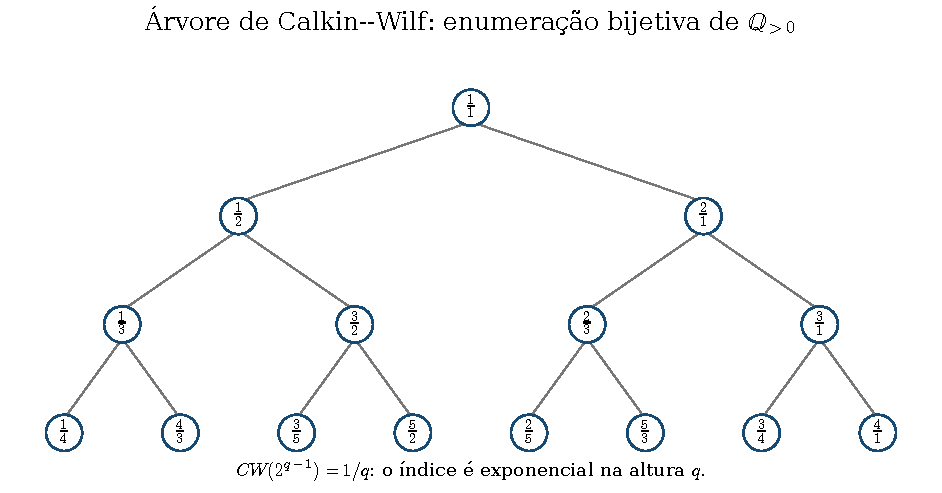
\includegraphics[width=.86\linewidth]{fig02_calkin_wilf.pdf}
 \caption{A enumeração de Calkin--Wilf é bijetiva, mas o endereço de $1/q$ cresce exponencialmente com sua altura. A ordenação por altura mantém o endereço polinomial; a \cref{sec:complexity} mostra que ela é, além disso, minimax-ótima em comprimento no pior caso para o calibre fixado.}
 \label{fig:cw-pt}
\end{figure}

\section{Células diádicas e operador gerador}
\label{sec:generator}

\subsection{Células, posse e centros}

Para $k\in\Nzero$ e $m\in\mathbb{Z}$, sejam
\begin{equation}
 J_{k,m}=[m2^{-k},(m+1)2^{-k}],\qquad
 J_{k,m}^{\own}=[m2^{-k},(m+1)2^{-k}),
 \label{eq:dyadic-cells}
\end{equation}
e
\begin{equation}
 x_0(k,m)=\left(m+\frac12\right)2^{-k}=\frac{2m+1}{2^{k+1}}.
 \label{eq:dyadic-center}
\end{equation}
A célula fechada sustenta o segmento; a versão semiaberta atribui cada fronteira a um único proprietário. Escreva
\[
 \mathbb{D}=\{j2^{-K}:j\in\mathbb{Z},\ K\in\Nzero\},\qquad
 \Dmid=\mathbb{D}\setminus\mathbb{Z}.
\]

\begin{lemma}[estrutura diádica]\label{lem:dyadic}
Para cada $k$, as células $J_{k,m}^{\own}$ particionam $\mathbb{R}$ e
\begin{equation}
 J_{k,m}=J_{k+1,2m}\cup J_{k+1,2m+1},\qquad |J_{k,m}|=2^{-k}.
 \label{eq:refinement}
\end{equation}
O mapa $(k,m)\mapsto x_0(k,m)$ é uma bijeção de $\Nzero\times\mathbb{Z}$ sobre $\Dmid$, que é denso em $\mathbb{R}$.
\end{lemma}

\begin{proof}
Para $x\in\mathbb{R}$, o único índice de posse na escala $k$ é $m=\lfloor2^kx\rfloor$; isso prova a partição. A identidade de refinamento decorre de cindir $[2m2^{-(k+1)},(2m+2)2^{-(k+1)}]$ em seu ponto médio.

Pela \eqref{eq:dyadic-center}, o centro tem numerador ímpar e denominador reduzido $2^{k+1}\ge2$, logo pertence a $\Dmid$. Reciprocamente, cada $x\in\Dmid$ possui forma reduzida única $j/2^K$, com $K\ge1$ e $j$ ímpar; tomando $k=K-1$ e $m=(j-1)/2$, obtém-se $x=x_0(k,m)$. A mesma unicidade prova a injetividade. Por fim, os centros de escala $k$ estão espaçados por $2^{-k}$; escolhendo o mais próximo de um real dado, a distância tende a zero com $k$, o que prova a densidade.
\end{proof}

A convenção de posse, os centros e o primeiro passo de refinamento aparecem
esquematicamente na \cref{fig:dyadic-pt}.

\begin{figure}[t]
 \centering
 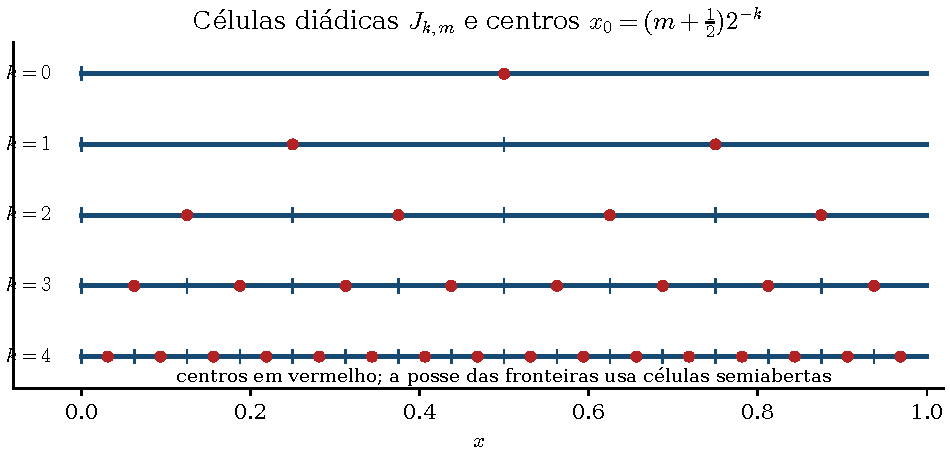
\includegraphics[width=.91\linewidth]{fig01_diadicos.pdf}
 \caption{Células diádicas, centros e convenção semiaberta de posse.}
 \label{fig:dyadic-pt}
\end{figure}

\subsection{Retas ancoradas e descompactação}

Dados $x_0,y_0\in\mathbb{R}$ e $s\neq0$, a reta ancorada é
\begin{equation}
 \ell(x)=y_0+s(x-x_0)=a+bx,\qquad b=s,\quad a=y_0-sx_0.
 \label{eq:anchored-line}
\end{equation}
Para $n\in\Nzero$, aplique sucessivamente a inversa do pareamento:
\begin{equation}
 (u,v)=\pi^{-1}(n),\qquad (k,\mu)=\pi^{-1}(u),\qquad (r,t)=\pi^{-1}(v).
 \label{eq:unpack}
\end{equation}

\begin{lemma}\label{lem:unpack}
O mapa $n\mapsto(k,\mu,r,t)$ de \eqref{eq:unpack} é uma bijeção de $\Nzero$ sobre $\Nzero^4$.
\end{lemma}

\begin{proof}
Sua inversa explícita é
\[
 (k,\mu,r,t)\longmapsto \pi\bigl(\pi(k,\mu),\pi(r,t)\bigr),
\]
uma composição de bijeções pelo \cref{lem:cantor}.
\end{proof}

Defina
\begin{equation}
 m=Z(\mu),\quad x_{0,n}=x_0(k,m),\quad y_{0,n}=Q(r),\quad s_n=Q^{\!*}(t),
 \label{eq:local-parameters}
\end{equation}
e converta para a forma global por
\begin{equation}
 b_n=s_n,\qquad a_n=y_{0,n}-s_nx_{0,n}.
 \label{eq:global-parameters}
\end{equation}
Se $x_L=m2^{-k}$ e $x_R=(m+1)2^{-k}$, ponha
\begin{equation}
 c_n=\min\{\ell_n(x_L),\ell_n(x_R)\},\qquad
 d_n=\max\{\ell_n(x_L),\ell_n(x_R)\}.
 \label{eq:range}
\end{equation}

\begin{definition}[gerador e biblioteca]\label{def:generator}
Se $\Intervals$ é o conjunto dos intervalos fechados não degenerados de $\mathbb{R}$, defina
\begin{equation}
 \Gamma:\Nzero\to\mathbb{R}\times(\mathbb{R}\setminus\{0\})\times\Intervals,
 \qquad \Gamma(n)=(a_n,b_n,[c_n,d_n]).
 \label{eq:generator}
\end{equation}
A biblioteca é $\Library=\Gamma(\Nzero)$. O átomo de endereço $n$ é a restrição de $\ell_n$ à célula $J_{k(n),m(n)}$.
\end{definition}

Como $s_n\neq0$ e $x_L\neq x_R$, o intervalo em \eqref{eq:range} é não degenerado, de modo que \eqref{eq:generator} está bem definido.

A exclusão da inclinação nula é estrutural, e não apenas uma convenção de
parametrização. É precisamente $b_n\neq0$ que torna a interface global
invertível no eixo espacial e permite recuperar a célula pela fórmula
\eqref{eq:preimage-intro}. Se fossem admitidas peças constantes, a imagem
$[c_n,d_n]$ degeneraria em um ponto e deixaria de codificar o intervalo de
origem. A extensão marcada $\Library^\square$, introduzida na
\cref{sec:regularized-reversibility}, é usada somente como dispositivo auxiliar
em resultados de reversão que precisam representar regiões planas; ela não
substitui a biblioteca original $\Library$ nem sua semântica de endereçamento.

Para uma interface global $\Gamma(n)=(a_n,b_n,[c_n,d_n])$, defina sua
pré-imagem espacial por
\begin{equation}
 I_n^x=\left[
 \min\!\left\{\frac{c_n-a_n}{b_n},\frac{d_n-a_n}{b_n}\right\},
 \max\!\left\{\frac{c_n-a_n}{b_n},\frac{d_n-a_n}{b_n}\right\}
 \right].
 \label{eq:preimage-intro}
\end{equation}

\subsection{Recuperação da célula e endereço canônico}

\begin{lemma}[validade espacial exata]\label{lem:cell-recovery}
Para todo $n\in\Nzero$, o intervalo $I_n^x$ definido em \eqref{eq:preimage-intro} satisfaz
\[
 I_n^x=J_{k(n),m(n)}.
\]
\end{lemma}

\begin{proof}
Como $b_n\neq0$, $\ell_n$ é uma bijeção afim estritamente monótona. Sua restrição a $[x_L,x_R]$ tem imagem $[c_n,d_n]$ por \eqref{eq:range}; logo $\ell_n^{-1}([c_n,d_n])=[x_L,x_R]$. Os dois quocientes em \eqref{eq:preimage-intro} são precisamente $\ell_n^{-1}(c_n)$ e $\ell_n^{-1}(d_n)$, possivelmente em ordem invertida quando $b_n<0$.
\end{proof}

\begin{theorem}[unicidade do endereço]\label{thm:injective}
$\Gamma$ é injetiva. Portanto, é uma bijeção de $\Nzero$ sobre $\Library$ e cada átomo tem um único endereço.
\end{theorem}

\begin{proof}
Suponha $\Gamma(n)=\Gamma(n')=(a,b,[c,d])$. Por \cref{lem:cell-recovery}, a tripla recupera a célula comum $J=[x_L,x_R]$. Seu comprimento determina unicamente $k=-\log_2|J|$, e $m=2^kx_L$. Assim, também se recupera $x_0=(m+1/2)2^{-k}$. A inclinação local é $s=b$ e o valor ancorado é $y_0=a+bx_0$.

Pelas bijeções dos \cref{lem:dyadic,lem:integers,lem:rational-rank}, os dados $(x_0,y_0,s)$ determinam unicamente $(k,\mu,r,t)$. O \cref{lem:unpack} determina então um único $n$. Logo $n=n'$.
\end{proof}

Em uma fronteira, duas células fechadas podem estar ativas. A célula semiaberta escolhe uma proprietária; em uma montagem contínua, as duas peças têm o mesmo valor no nó e essa escolha não altera a função.

\begin{theorem}[dicionário de jatos racionais]\label{thm:dictionary}
O mapa
\begin{equation}
 n\longmapsto(x_{0,n},y_{0,n},s_n)
 \label{eq:dictionary}
\end{equation}
é uma bijeção de $\Nzero$ sobre $\Dmid\times\mathbb{Q}\times\Qstar$. Sua imagem é densa em $\mathbb{R}^3$.
\end{theorem}

\begin{proof}
A bijetividade resulta da composição das bijeções em \eqref{eq:unpack}--\eqref{eq:local-parameters}. A densidade decorre da densidade de $\Dmid$, de $\mathbb{Q}$ e de $\Qstar$ em $\mathbb{R}$, aplicada coordenada a coordenada na norma do máximo.
\end{proof}

O dicionário \eqref{eq:dictionary} parametriza todos os 1-jatos com centro
diádico não inteiro, valor racional e derivada racional não nula. A
aproximação global resulta das montagens contínuas desses dados locais,
introduzidas na seção seguinte.

\section{Montagens e densidade em espaços de funções contínuas}
\label{sec:assemblies}

\begin{definition}[montagem contínua]\label{def:assembly}
Se $K=[\alpha,\beta]$ é um intervalo compacto não degenerado, $\Aclass(K)$ é o conjunto das funções $g\in C(K)$ para as quais existe uma coleção finita $\Lambda$ de células diádicas, com interiores disjuntos e união contendo $K$, e endereços $n(J)$, $J\in\Lambda$, tais que
\begin{equation}
 g|_{J\cap K}=\ell_{n(J)}|_{J\cap K},
 \label{eq:assembly}
\end{equation}
com valores coincidentes nas fronteiras compartilhadas.
\end{definition}

Para $f\in C(K)$, denote o módulo de continuidade por
\begin{equation}
 \omega(f;\delta)=\sup\{|f(x)-f(y)|:x,y\in K,\ |x-y|\le\delta\}.
\end{equation}

A densidade por interpolantes afins e a teoria de splines lineares são
clássicas \citep{deboor2001,powell1981,schumaker2007}. O resultado seguinte
registra o ponto adicional necessário aqui: nós diádicos, valores racionais e
inclinações não nulas podem ser impostos simultaneamente.

\begin{theorem}[densidade das montagens]\label{thm:density}
Para todo $f\in C[\alpha,\beta]$ e todo $\varepsilon>0$, existe $g\in\Aclass([\alpha,\beta])$ tal que
\[
 \|f-g\|_{\infty,[\alpha,\beta]}<\varepsilon.
\]
Todas as peças de $g$ pertencem a $\Library$ e têm inclinação não nula.
\end{theorem}

\begin{proof}
Estenda $f$ por constantes: $F(x)=f(\alpha)$ para $x<\alpha$, $F=f$ em $[\alpha,\beta]$ e $F(x)=f(\beta)$ para $x>\beta$. A extensão é uniformemente contínua. Escolha $k$ de modo que, com $h=2^{-k}$,
\begin{equation}
 \omega(F;h)<\varepsilon/2.
 \label{eq:modulus-choice}
\end{equation}
Tome os nós $t_j=jh$ desde $j_{\min}=\lfloor\alpha/h\rfloor$ até $j_{\max}=\lceil\beta/h\rceil$. Para cada $j$, escolha racional $v_j$ com $|v_j-F(t_j)|<\varepsilon/2$ e, sequencialmente, imponha $v_{j+1}\neq v_j$. Isso é possível porque cada intervalo aberto de escolha contém infinitos racionais e apenas um valor é proibido em cada passo.

Seja $g$ o interpolante linear dos pares $(t_j,v_j)$. Em $J_{k,j}$, sua inclinação é $(v_{j+1}-v_j)/h\in\Qstar$ e seu valor no centro é $(v_j+v_{j+1})/2\in\mathbb{Q}$. Pelo \cref{thm:dictionary}, a peça é o único átomo com esses parâmetros. Os valores nodais compartilhados tornam $g$ contínua.

Se $P_kF$ é o interpolante dos valores exatos, então, para $x=(1-\theta)t_j+\theta t_{j+1}$,
\[
 |F(x)-P_kF(x)|
 \le(1-\theta)|F(x)-F(t_j)|+\theta|F(x)-F(t_{j+1})|
 \le\omega(F;h)<\varepsilon/2.
\]
Além disso, $P_kF-g$ é linear em cada célula e seus valores nodais têm módulo menor que $\varepsilon/2$, logo $\|P_kF-g\|_\infty<\varepsilon/2$. A desigualdade triangular conclui.
\end{proof}

O número de células dessa cobertura uniforme é
\begin{equation}
 N_k=\lceil\beta2^k\rceil-\lfloor\alpha2^k\rfloor
     =(\beta-\alpha)2^k+O(1).
 \label{eq:cell-count}
\end{equation}

A \cref{fig:assemblies-pt} mostra duas dessas racionalizações sobre malhas
diádicas e identifica as peças efetivamente pertencentes a $\Library$.

\begin{figure}[t]
 \centering
 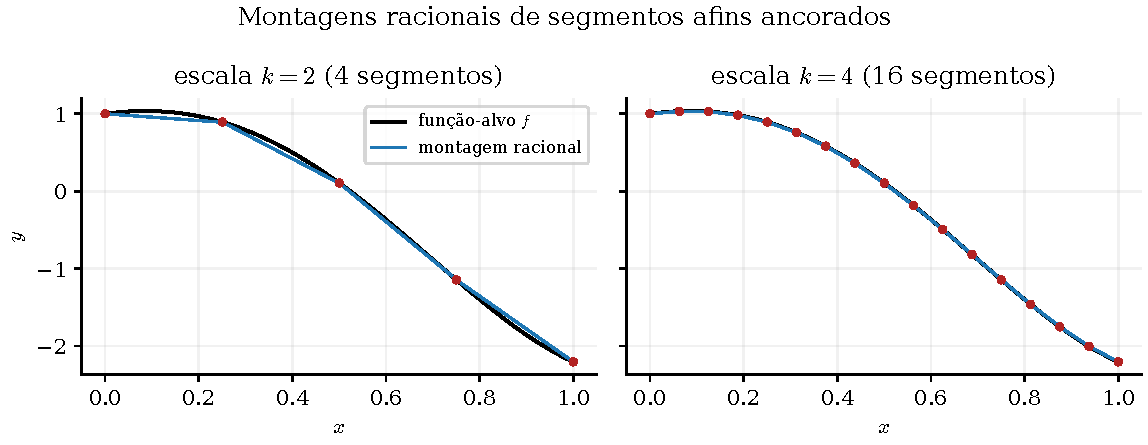
\includegraphics[width=.94\linewidth]{fig03_aproximacao.pdf}
 \caption{Montagens com valores nodais racionalizados em uma grade diádica; cada segmento exibido é um átomo de $\Library$.}
 \label{fig:assemblies-pt}
\end{figure}

\subsection{Equivalência exata com redes ReLU racionais}

Escreva $\rho(z)=z_+=\max\{0,z\}$. A relação entre montagens e redes
lineares por partes pode ser formulada sem aproximação e sem parâmetros reais
ocultos. A identidade em hinges usada a seguir é clássica na representação de
funções lineares por partes por redes ReLU
\citep{yarotsky2017,devorehaninpetrova2021,daubechies2022}; o conteúdo
específico aqui é sua compatibilidade exata com os nós diádicos, os parâmetros
racionais, a recuperação das células e a restrição de inclinação não nula.

\begin{theorem}[equivalência montagem--ReLU racional]
\label{thm:assembly-relu}
Seja $g\in\Aclass(K)$ dada por $N$ folhas consecutivas, com nós
$t_0<t_1<\cdots<t_N$ e inclinação racional não nula $s_j$ em
$[t_j,t_{j+1}]\cap K$, $0\le j<N$. Então, em $K$,
\begin{equation}
 g(x)=g(t_0)+s_0(x-t_0)
      +\sum_{j=1}^{N-1}(s_j-s_{j-1})\rho(x-t_j).
 \label{eq:assembly-relu}
\end{equation}
Depois de expandido o primeiro termo afim, todos os coeficientes são
racionais, todos os pontos de quebra internos são diádicos e
\eqref{eq:assembly-relu} é uma rede ReLU rasa normalizada com $N-1$ unidades
hinge e um termo afim de saída. Unidades cujo peso de saída é zero podem ser
removidas.

Reciprocamente, seja
\begin{equation}
 R(x)=c+qx+\sum_{j=1}^{M}a_j\rho(x-\tau_j),
 \qquad c,q,a_j\in\mathbb Q,\quad \tau_j\in\mathbb D,
 \label{eq:normalized-relu}
\end{equation}
com nós distintos. Suponha que $K$ admita uma cobertura por células diádicas
compatível com os $\tau_j$, que os valores nodais sejam racionais e que cada
inclinação local
\begin{equation}
 q+\sum_{\tau_j<x}a_j
 \label{eq:relu-local-slope}
\end{equation}
seja não nula. Então $R|_K\in\Aclass(K)$. Uma malha diádica uniforme que
refine todos os $\tau_j$ fornece essa montagem explicitamente.
\end{theorem}

\begin{proof}
Na primeira folha, o lado direito de \eqref{eq:assembly-relu} tem valor
$g(t_0)$ em $t_0$ e inclinação $s_0$. Ao atravessar $t_j$, a derivada ganha
exatamente $s_j-s_{j-1}$; por indução, sua inclinação na folha $j$ é $s_j$.
Como ambos os lados são contínuos e coincidem no primeiro nó, coincidem em
todo $K$. Cada $s_j$ é racional. Os nós internos são fronteiras de células
diádicas, e o intercepto do primeiro átomo é racional por
\eqref{eq:global-parameters}; logo a forma expandida tem somente parâmetros
racionais.

Para a recíproca, refine uma grade diádica até que cada $\tau_j$ seja uma
fronteira. Em qualquer célula aberta da grade, \eqref{eq:normalized-relu} é
afim, com inclinação \eqref{eq:relu-local-slope}. O valor no centro da célula
é racional, pois o centro, os nós e todos os coeficientes são racionais. A
hipótese de inclinação não nula permite aplicar o
\cref{thm:dictionary}, que fornece um único átomo da biblioteca nessa célula.
A continuidade de $R$ faz os valores coincidirem nas fronteiras. A união das
peças é, portanto, uma montagem no sentido da \cref{def:assembly}.
\end{proof}

A racionalidade dos valores nodais na recíproca é automática na forma
normalizada \eqref{eq:normalized-relu}; ela foi enunciada separadamente para
deixar explícita a interface exigida de uma parametrização de rede mais geral.
A condição de inclinação não nula não é cosmética: se uma inclinação local
fosse zero, a peça correspondente não teria suporte recuperável pela
\cref{lem:cell-recovery}. Se a arquitetura não oferecer a conexão afim direta,
o termo linear pode ser realizado por
$x=\rho(x)-\rho(-x)$, ao custo de duas unidades adicionais, mantendo o viés
constante na saída.

\begin{proposition}[parâmetros e altura]
\label{prop:relu-complexity}
Na forma normalizada, a conversão de uma montagem com $N$ folhas armazena
$2N$ racionais: o intercepto e a inclinação iniciais, mais um nó e um salto de
inclinação para cada uma das $N-1$ unidades. Se todos os átomos têm altura no
máximo $H\ge2$, a altura máxima dos parâmetros produzidos satisfaz
\begin{equation}
 H_{\mathrm{ReLU}}\le 2^{H+1}H^2.
 \label{eq:relu-height-bound}
\end{equation}
\end{proposition}

\begin{proof}
Há $N-1$ pares $(t_j,s_j-s_{j-1})$, além dos dois parâmetros afins. Pela
definição de altura atômica, $\height(s_j)\le H$, os nós satisfazem
$\height(t_j)\le2^H$, e a forma geral do
\cref{lem:height-arithmetic} dá
$\height(s_j-s_{j-1})\le2H^2$. Para o intercepto inicial, escreva
$a=y_0-sx_0$. Como $\height(x_0)\le2^H$,
\[
 \height(a)\le2\height(y_0)\height(sx_0)
 \le2^{H+1}H^2.
\]
Isso prova \eqref{eq:relu-height-bound}. Como
os demais parâmetros são produtos ou somas dos mesmos dados, essa cota também
garante que a conversão é efetiva em aritmética racional exata.
\end{proof}

O \cref{thm:assembly-relu} estabelece identidade funcional entre montagens e
redes rasas. Os custos de codificação, busca e interpretação constituem
questões distintas. Após fixar códigos prefix-free executáveis, o
\cref{thm:coding-formats} separa o custo de transmitir diádicos como pares
estruturais daquele de expandi-los como frações reduzidas.

A \cref{fig:relu-equivalence-pt} exibe uma instância cujos pesos foram
obtidos pelo mesmo conversor racional exato usado na verificação computacional.

\begin{figure}[t]
 \centering
 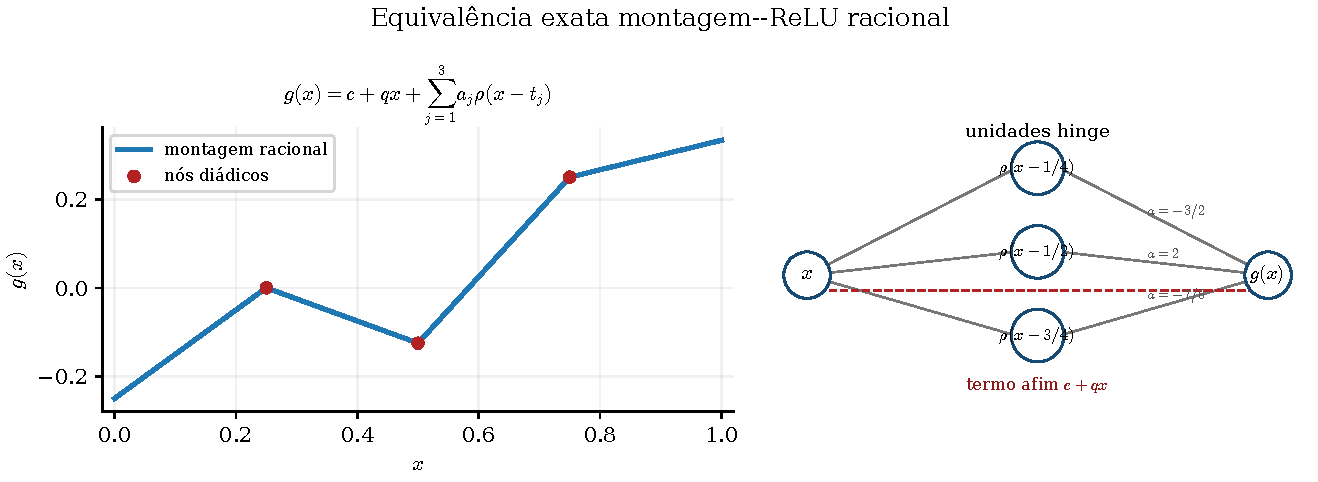
\includegraphics[width=.96\linewidth]{fig07_relu.pdf}
 \caption{Uma montagem racional com quatro folhas e sua rede ReLU rasa
 correspondente. O gráfico e os pesos do diagrama são gerados pelo mesmo
 conversor exato usado nos testes.}
 \label{fig:relu-equivalence-pt}
\end{figure}

\subsection{Relação com o 1-jato de Taylor}

Se $J_{k,m}$ tem centro $x_0$ e largura $h$, o 1-jato de $f\in C^2(J_{k,m})$ é
\[
 T_{x_0}f(x)=f(x_0)+f'(x_0)(x-x_0).
\]

\begin{proposition}[pertencimento e aderência]\label{prop:jet}
Se $f(x_0)\in\mathbb{Q}$ e $f'(x_0)\in\Qstar$, então $T_{x_0}f$ é o átomo de $\Library$ associado à célula. Em geral, para todo $\delta>0$ existem $q_0\in\mathbb{Q}$ e $q_1\in\Qstar$ tais que $\ell_q(x)=q_0+q_1(x-x_0)$ satisfaz
\begin{align}
 \|T_{x_0}f-\ell_q\|_{\infty,J_{k,m}}&<\delta,\label{eq:jet-close}\\
 \|f-\ell_q\|_{\infty,J_{k,m}}&\le \frac{h^2}{8}\|f''\|_{\infty,J_{k,m}}+\delta.
 \label{eq:jet-error}
\end{align}
\end{proposition}

\begin{proof}
No primeiro caso, $(x_0,f(x_0),f'(x_0))$ pertence ao contradomínio do \cref{thm:dictionary}. No caso geral, escolha $q_0$ com $|f(x_0)-q_0|<\delta/2$ e $q_1\neq0$ com $|f'(x_0)-q_1|<\delta/h$. Como $|x-x_0|\le h/2$, obtém-se \eqref{eq:jet-close}. O resto integral de Taylor fornece
\[
 |f(x)-T_{x_0}f(x)|
 =\left|\int_{x_0}^{x}(x-t)f''(t)\dd t\right|
 \le\frac{|x-x_0|^2}{2}\|f''\|_\infty
 \le\frac{h^2}{8}\|f''\|_\infty.
\]
A desigualdade triangular prova \eqref{eq:jet-error}.
\end{proof}

Assim, jatos reais arbitrários pertencem à aderência local da biblioteca racional; não pertencem necessariamente à própria biblioteca.

\section{Taxas uniformes e constante assintótica}
\label{sec:rates}

Para $f\in C^2[\alpha,\beta]$, use a extensão
\begin{equation}
F(x)=
\begin{cases}
f(\alpha)+f'(\alpha)(x-\alpha)+\tfrac12f''(\alpha)(x-\alpha)^2,&x<\alpha,\\
f(x),&\alpha\le x\le\beta,\\
f(\beta)+f'(\beta)(x-\beta)+\tfrac12f''(\beta)(x-\beta)^2,&x>\beta.
\end{cases}
\label{eq:c2-extension}
\end{equation}
Então $F\in C^2(\mathbb{R})$ e $\|F''\|_{\infty,\mathbb{R}}=\|f''\|_{\infty,[\alpha,\beta]}$. Seja $P_kF$ o interpolante nos nós $j2^{-k}$.

A fórmula local do resto da interpolação linear e a constante $1/8$ que dela
decorre são fatos clássicos da aproximação por splines
\citep{deboor2001,powell1981,schumaker2007}. A afirmação abaixo também prova o
limite uniforme e preserva a constante sob a racionalização específica da
biblioteca.

\begin{theorem}[cota aguda e limite]\label{thm:uniform}
Ponha $h=2^{-k}$ e $M=\|f''\|_{\infty,[\alpha,\beta]}$. Então
\begin{equation}
 \|f-P_kF\|_{\infty,[\alpha,\beta]}\le\frac{h^2M}{8},
 \label{eq:uniform-bound}
\end{equation}
e
\begin{equation}
 \lim_{k\to\infty}\frac{8}{h^2}\|f-P_kF\|_{\infty,[\alpha,\beta]}=M.
 \label{eq:uniform-limit}
\end{equation}
Além disso, para todo $\delta>0$ existe $g_{k,\delta}\in\Aclass([\alpha,\beta])$ com
\begin{equation}
 \|f-g_{k,\delta}\|_\infty\le\frac{h^2M}{8}+\delta.
 \label{eq:rational-rate}
\end{equation}
\end{theorem}

\begin{proof}
Em uma célula $[x_L,x_R]$ de largura $h$, ponha $e=F-P_kF$. Para $x\in(x_L,x_R)$, a função
\[
 \psi(t)=e(t)-\frac{(t-x_L)(t-x_R)}{(x-x_L)(x-x_R)}e(x)
\]
anula-se em $x_L,x,x_R$. Três aplicações de Rolle produzem $\xi_x\in(x_L,x_R)$ com $\psi''(\xi_x)=0$; portanto
\begin{equation}
 F(x)-P_kF(x)=\frac12F''(\xi_x)(x-x_L)(x-x_R).
 \label{eq:interpolation-remainder}
\end{equation}
O módulo do produto é no máximo $h^2/4$, com igualdade no centro, o que prova \eqref{eq:uniform-bound}.

Se $M=0$, \eqref{eq:uniform-limit} é imediata. Se $M>0$, escolha $x_*\in[\alpha,\beta]$ com $|f''(x_*)|=M$. Para cada $k$ suficientemente grande, escolha um centro de escala $k$, $z_k\in[\alpha,\beta]$, com $z_k\to x_*$. Avaliando \eqref{eq:interpolation-remainder} em $z_k$,
\[
 |F(z_k)-P_kF(z_k)|=\frac{h^2}{8}|F''(\xi_k)|,
\]
onde $\xi_k$ pertence à célula de $z_k$. O diâmetro da célula tende a zero, logo $\xi_k\to x_*$ e $|F''(\xi_k)|\to M$. Isso dá o limite inferior; \eqref{eq:uniform-bound} fornece o superior.

Para a última afirmação, racionalize todos os valores nodais da cobertura finita com erro menor que $\delta$ e mantenha valores adjacentes distintos, como no \cref{thm:density}. O interpolante resultante é uma montagem e dista menos que $\delta$ de $P_kF$ em norma uniforme. A desigualdade triangular conclui.
\end{proof}

\begin{corollary}[preservação da constante]\label{cor:rational-sharp}
Existe uma sequência $g_k\in\Aclass([\alpha,\beta])$ tal que
\[
 \lim_{k\to\infty}\frac{8}{h^2}\|f-g_k\|_\infty=M.
\]
\end{corollary}

\begin{proof}
Na construção do \cref{thm:uniform}, escolha erros nodais $\delta_k=o(h^2)$. Então
\[
 \bigl|\|f-g_k\|_\infty-\|f-P_kF\|_\infty\bigr|
 \le\|g_k-P_kF\|_\infty<\delta_k.
\]
Divida por $h^2/8$ e aplique \eqref{eq:uniform-limit}.
\end{proof}

Com $N_k$ de \eqref{eq:cell-count}, $h=(\beta-\alpha)N_k^{-1}(1+O(N_k^{-1}))$ e, portanto,
\begin{equation}
 \|f-P_kF\|_\infty
 \le \frac{(\beta-\alpha)^2M}{8}N_k^{-2}\bigl(1+O(N_k^{-1})\bigr).
 \label{eq:n-rate}
\end{equation}
Quando os extremos já são nós da malha, o termo de borda desaparece.

A \cref{tab:exp-pt} registra os valores exatos para $e^x$, enquanto a
\cref{fig:exp-pt} evidencia a convergência da razão para a constante aguda.

\begin{table}[t]
\centering
\caption{Erro exato do interpolante de $e^x$ em $[0,1]$.}
\label{tab:exp-pt}
\begin{tabular}{rrrr}
\toprule
$k$ & erro exato & $2^{-2k}e/8$ & razão\\
\midrule
2  & $1{,}8774\times10^{-2}$ & $2{,}1237\times10^{-2}$ & $0{,}8840$\\
4  & $1{,}2866\times10^{-3}$ & $1{,}3273\times10^{-3}$ & $0{,}9693$\\
6  & $8{,}2310\times10^{-5}$ & $8{,}2955\times10^{-5}$ & $0{,}9922$\\
8  & $5{,}1746\times10^{-6}$ & $5{,}1847\times10^{-6}$ & $0{,}9980$\\
10 & $3{,}2389\times10^{-7}$ & $3{,}2404\times10^{-7}$ & $0{,}9995$\\
\bottomrule
\end{tabular}
\end{table}

\begin{figure}[t]
 \centering
 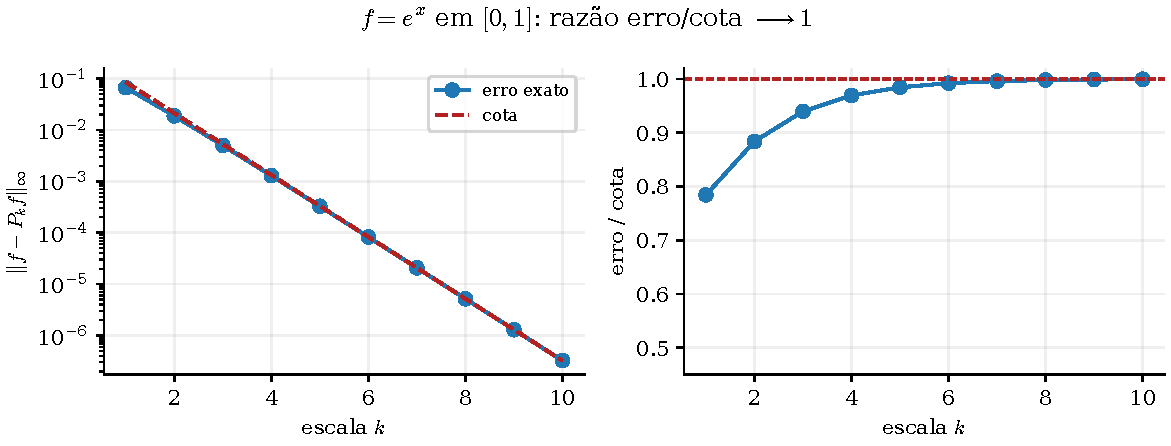
\includegraphics[width=.92\linewidth]{fig04_exp.pdf}
 \caption{A razão entre o erro exato e a cota converge a $1$, em concordância com \eqref{eq:uniform-limit}.}
 \label{fig:exp-pt}
\end{figure}

\section{Árvores diádicas, nós livres e regularidade de Besov}
\label{sec:dyadic-trees}

\subsection{Partições em árvore}

Se $K$ é uma célula diádica, uma partição em árvore $\Lambda$ é o conjunto de folhas de uma subárvore diádica finita com raiz $K$. Seja $P_\Lambda f$ o interpolante de $f$ nos extremos das folhas e defina
\begin{equation}
 \sigma_N^{\mathrm{dia}}(f)_\infty
 =\inf\{\|f-P_\Lambda f\|_{\infty,K}:\Lambda\text{ árvore},\ |\Lambda|\le N\}.
 \label{eq:sigma-dyadic}
\end{equation}

\begin{theorem}[taxa garantida em árvores]\label{thm:tree-rate}
Se $f\in C^2(K)$, $L=|K|$, $M=\|f''\|_{\infty,K}$ e $N\ge2$, então
\begin{equation}
 \sigma_N^{\mathrm{dia}}(f)_\infty\le\frac{ML^2}{2N^2}.
 \label{eq:tree-general}
\end{equation}
Se $N=2^r$, a constante melhora para
\begin{equation}
 \sigma_N^{\mathrm{dia}}(f)_\infty\le\frac{ML^2}{8N^2}.
 \label{eq:tree-power}
\end{equation}
Para qualquer árvore finita $\Lambda$ e $\delta>0$, há uma montagem racional na mesma árvore cujo erro é menor que $\|f-P_\Lambda f\|_\infty+\delta$.
\end{theorem}

\begin{proof}
Tome $r=\lfloor\log_2N\rfloor$ e refine $K$ uniformemente $r$ vezes. Há $2^r\le N$ folhas de largura $L2^{-r}$. Aplicando \eqref{eq:interpolation-remainder} em cada folha,
\[
 \|f-P_\Lambda f\|_\infty\le\frac{ML^2}{8}4^{-r}.
\]
Se $N=2^r$, resulta \eqref{eq:tree-power}. Em geral, $2^r>N/2$, logo $4^{-r}<4N^{-2}$, o que dá \eqref{eq:tree-general}. Para a racionalização, ordene os nós, aproxime os valores de $f$ por racionais compartilhados com erro menor que $\delta$ e evite igualdade entre vizinhos. Em cada folha, a diferença entre o interpolante exato e o racional é combinação convexa dos erros nodais; o argumento do \cref{thm:density} identifica cada peça como átomo.
\end{proof}

\subsection{Referência assintótica com nós livres}

Se $E_N^{\mathrm{lv}}(f)$ é o menor erro de interpolação linear com $N$
subintervalos e nós arbitrários, o regime de nós livres fornece a referência
contínua para comparação com árvores diádicas
\citep{deboor1973variable,burchard1974,deboor2001,powell1981,schumaker2007}.

\begin{theorem}[cota assintótica com nós livres]\label{thm:free-knots}
Para $f\in C^2[\alpha,\beta]$,
\begin{equation}
 \limsup_{N\to\infty}N^2E_N^{\mathrm{lv}}(f)
 \le\frac18\left(\int_\alpha^\beta |f''(x)|^{1/2}\dd x\right)^2.
 \label{eq:free-knot}
\end{equation}
\end{theorem}

\begin{proof}
Fixe $\eta>0$ e ponha $\rho_\eta=(|f''|+\eta)^{1/2}$ e $I_\eta=\int_\alpha^\beta\rho_\eta$. Como $\rho_\eta$ é contínua e estritamente positiva, existem nós $\alpha=x_{N,0}<\cdots<x_{N,N}=\beta$ tais que
\[
 \int_{x_{N,j-1}}^{x_{N,j}}\rho_\eta=I_\eta/N.
\]
O comprimento máximo das células tende uniformemente a zero. Em $J_j=[x_{N,j-1},x_{N,j}]$, \eqref{eq:interpolation-remainder} e $|f''|\le\rho_\eta^2$ dão
\[
 \|f-P_{J_j}f\|_{\infty,J_j}
 \le\frac18\left(\frac{I_\eta}{N}\right)^2
 \left(\frac{\sup_{J_j}\rho_\eta}{\inf_{J_j}\rho_\eta}\right)^2.
\]
Por continuidade uniforme e positividade, a última razão converge uniformemente a $1$. Assim,
\[
 \limsup_{N\to\infty}N^2E_N^{\mathrm{lv}}(f)\le I_\eta^2/8.
\]
Fazendo $\eta\downarrow0$ e usando convergência dominada, obtém-se \eqref{eq:free-knot}.
\end{proof}

A constante em \eqref{eq:free-knot} pertence ao regime de nós livres. A
constante sob restrição diádica será determinada na
\cref{sec:dyadic-asymptotic}; é essa comparação, retomada explicitamente nos
\cref{thm:general-dyadic-envelope,thm:quadratic-dyadic-constant}, que mede o
custo da restrição de malha.

\subsection{Estimativa direta na escala de Besov}

As relações diretas e inversas entre aproximação por partes, splines e classes
de suavidade têm uma tradição ampla
\citep{birman1967,petrushev1988,devorepopov1988}. A formulação abaixo fixa a
escala estritamente diádica e o interpolante linear usados neste artigo.

Para $f\in C(K)$, defina
\begin{equation}
 \omega_2(f,t)_{\infty,K}
 =\sup_{\substack{0<h\le t\\x,x+2h\in K}}
 |f(x+2h)-2f(x+h)+f(x)|,
\end{equation}
e, para $0<s<2$,
\begin{equation}
 |f|_{B^s_{\infty,\infty}(K)}
 =\sup_{0<t\le|K|}t^{-s}\omega_2(f,t)_{\infty,K}.
 \label{eq:besov-seminorm}
\end{equation}

\begin{theorem}[estimativa direta]\label{thm:besov}
Se $0<s<2$, $|K|=L$ e o seminorma em \eqref{eq:besov-seminorm} é finito, então, para $N\ge2$,
\begin{equation}
 \sigma_N^{\mathrm{dia}}(f)_\infty
 \le C_sL^s|f|_{B^s_{\infty,\infty}(K)}N^{-s},
 \label{eq:besov-rate}
\end{equation}
onde $C_s$ independe de $f$ e $N$. Para todo $\delta>0$, uma montagem racional com no máximo $N$ folhas alcança o lado direito de \eqref{eq:besov-rate} acrescido de $\delta$.
\end{theorem}

\begin{proof}
A desigualdade de Whitney de ordem dois afirma que existe constante universal $C_W$ tal que, em todo intervalo $J$ \citep{whitney1957,devore1998},
\[
 E_1(f;J)_\infty:=\inf_{\ell\ \mathrm{afim}}\|f-\ell\|_{\infty,J}
 \le C_W\omega_2(f,|J|)_{\infty,J}.
\]
O interpolante de extremos $P_J$ reproduz funções afins e tem norma de operador no máximo $1$. Logo, para toda $\ell$ afim,
\[
 \|f-P_Jf\|_\infty
 \le\|f-\ell\|_\infty+\|P_J(f-\ell)\|_\infty
 \le2\|f-\ell\|_\infty.
\]
Tomando o ínfimo e observando que o módulo em $J\subset K$ não excede o de $K$,
\[
 \|f-P_Jf\|_{\infty,J}
 \le2C_W|J|^s|f|_{B^s_{\infty,\infty}(K)}.
\]
Refine $K$ uniformemente $r=\lfloor\log_2N\rfloor$ vezes. As folhas têm largura $L2^{-r}<2L/N$, e o máximo das estimativas locais prova \eqref{eq:besov-rate} com $C_s=2^{s+1}C_W$. A racionalização segue do último enunciado do \cref{thm:tree-rate}.
\end{proof}

O \cref{thm:besov} estabelece a direção regularidade--taxa. As
\cref{sec:approximation-classes,sec:direct-height,sec:regularized-reversibility}
incorporam altura aritmética, demonstram a recíproca crítica do erro bruto e
obtêm a caracterização regularizada completa. Para bases de ondaletas, as
caracterizações correspondentes seguem hipóteses próprias
\citep{devore1998,cohen2001}.

\section{Refinamento diádico adaptativo certificado}
\label{sec:adaptive}

Três amostras de uma função não fornecem, sem hipótese adicional, um limitante do erro em todo o intervalo. A garantia adaptativa será baseada em majorantes locais certificados de $|F''|$, não em diferenças segundas amostrais.

\subsection{Fechamento operacional por aritmética intervalar}

O majorante local pode ser construído, em vez de postulado, para uma gramática
explícita de funções. Seja $\mathcal E$ a menor classe de expressões que contém
$x$ e as constantes racionais e é fechada por soma, subtração, produto,
recíproco, $\exp$, $\sin$, $\cos$ e composição. Um recíproco só é admissível
em intervalos nos quais seu denominador não se anula. Essa classe contém os
polinômios, as funções racionais sem polos no domínio e as funções elementares
usadas nos experimentos.

Aqui composição significa substituição sintática: em $u\circ v$, cada folha
$x$ da árvore de $u$ é substituída pela árvore de $v$. Portanto toda expressão
composta volta a ser uma árvore das operações-base acima; composição não cria
um operador adicional nem um caso omitido na indução estrutural.

Escreva $\mathbb I_{\mathbb Q}$ para os intervalos fechados com extremos
racionais. A implementação pública
\begin{equation}
 \operatorname{BoundSecondDerivative}(E,J;P,d)
   =[\underline m_J,\overline m_J]\in\mathbb I_{\mathbb Q}
 \label{eq:bound-second-interface}
\end{equation}
usa precisão transcendental $P$ e profundidade de subdivisão $d$. Ela propaga
simultaneamente intervalos para $(E,E',E'')$, isto é, 2-jatos intervalares. Por
exemplo,
\begin{align*}
 (uv)''&=u''v+2u'v'+uv'',\\
 (u^{-1})''&=2(u')^2u^{-3}-u''u^{-2},\\
 (e^u)''&=e^u\bigl((u')^2+u''\bigr),\\
 (\sin u)''&=-\sin(u)(u')^2+\cos(u)u'',\\
 (\cos u)''&=-\cos(u)(u')^2-\sin(u)u''.
\end{align*}
As operações racionais são exatas. Para $\exp$, a redução do argumento a
$|z|\le1/2$ é seguida por uma soma de Taylor cujo resto é majorado por uma
série geométrica racional; para $\sin$ e $\cos$, usa-se o resto de Lagrange
racional e a interseção com $[-1,1]$. Depois, elevam-se $P$ e $d$ quando se
deseja reduzir a sobrestimação. Essa construção segue o princípio de inclusão
da aritmética intervalar validada \citep{moore2009,silva2025}.

\begin{lemma}[restos transcendentais com extremos racionais]
\label{lem:rational-transcendental-enclosures}
Se $I=[a,b]\in\mathbb I_{\mathbb Q}$, as rotinas descritas acima produzem
intervalos de extremos racionais que contêm $\exp(I)$, $\sin(I)$ e $\cos(I)$.
Mais explicitamente, para $0\le z\le1/2$ e $n\ge0$,
\begin{equation}
 0\le e^z-\sum_{j=0}^{n}\frac{z^j}{j!}
 \le
 \frac{z^{n+1}}{(n+1)!}
 \frac{1}{1-z/(n+2)}.
 \label{eq:exp-rational-tail}
\end{equation}
Se $R=\max\{|a|,|b|\}$ e
\begin{align*}
 P_n^{\sin}(z)&=\sum_{j=0}^{n}(-1)^j\frac{z^{2j+1}}{(2j+1)!},&
 P_n^{\cos}(z)&=\sum_{j=0}^{n}(-1)^j\frac{z^{2j}}{(2j)!},
\end{align*}
então, para todo $z\in I$,
\begin{align}
 |\sin z-P_n^{\sin}(z)|
 &\le \frac{R^{2n+2}}{(2n+2)!},
 &
 |\cos z-P_n^{\cos}(z)|
 &\le \frac{R^{2n+1}}{(2n+1)!}.
 \label{eq:trig-rational-remainders}
\end{align}
Avaliar os polinômios em $I$, inflar pelos respectivos restos e intersectar
com $[-1,1]$ preserva a inclusão.
\end{lemma}

\begin{proof}
Na série de $e^z$, o primeiro termo omitido é
$t_{n+1}=z^{n+1}/(n+1)!$. Para $j\ge n+1$, a razão entre termos consecutivos
é $z/(j+1)\le z/(n+2)<1$; a cauda é, portanto, majorada pela série geométrica
de primeiro termo $t_{n+1}$ e razão $z/(n+2)$, o que dá
\eqref{eq:exp-rational-tail}. Para um argumento racional $x$ arbitrário,
escolha $r$ com $z=|x|/2^r\le1/2$, aplique a inclusão anterior e eleve o
intervalo ao quadrado $r$ vezes; se $x<0$, tome o recíproco do intervalo
positivo obtido para $-x$. Em $I=[a,b]$, a monotonicidade de $e^x$ permite
usar o extremo inferior da inclusão em $a$ e o superior da inclusão em $b$.

As duas desigualdades em \eqref{eq:trig-rational-remainders} são o resto de
Lagrange dos polinômios de Maclaurin de graus $2n+1$ e $2n$, pois todas as
derivadas de seno e cosseno têm módulo no máximo $1$. A avaliação intervalar
contém a imagem de cada polinômio; inflar pelo raio do resto contém a função.
Como seno e cosseno já pertencem a $[-1,1]$, a interseção não remove nenhum
valor possível. Todas as operações, fatoriais e extremos envolvidos são
racionais.
\end{proof}

\begin{proposition}[correção do majorante intervalar]
\label{prop:interval-majorant}
Se $E\in\mathcal E$ define uma função $C^2$ em $J$ e a rotina
\eqref{eq:bound-second-interface} termina com sucesso, então
\begin{equation}
 E''(x)\in[\underline m_J,\overline m_J]\quad(x\in J),
 \qquad
 M_{\rm int}(J):=\max\{|\underline m_J|,|\overline m_J|\}
 \ge \|E''\|_{\infty,J}.
 \label{eq:interval-majorant}
\end{equation}
Se algum intervalo de denominador contém zero mesmo após a subdivisão
permitida, a rotina devolve falha e nenhum número é aceito como certificado.
Em particular, sua garantia nunca depende de amostragem.
\end{proposition}

\begin{proof}
Para constantes e para $x$, a inclusão é imediata. Soma, produto e recíproco
preservam inclusão pelas operações elementares de intervalos; o recíproco só
é executado quando zero está fora do intervalo do denominador. As fórmulas de
2-jatos acima e o \cref{lem:rational-transcendental-enclosures}
dão o passo de indução estrutural para toda expressão de $\mathcal E$.
Pela normalização sintática declarada antes do lema, uma composição genérica
já foi expandida nessa árvore e não acrescenta um caso independente.
Subdividir $J$ preserva a cobertura, e tomar o fecho convexo dos intervalos
obtidos em suas partes contém a união das imagens de $E''$. Isso prova a
primeira inclusão e, tomando módulos, \eqref{eq:interval-majorant}. A regra de
falha impede que uma divisão não validada produza uma falsa garantia.
\end{proof}

A certificação cobre as expressões para as quais os orçamentos $(P,d)$ fecham
a propagação intervalar sem polos. Formas naturais podem ser largas pelo
problema de dependência; subdivisão, formas centradas e Taylor intervalar
fornecem mecanismos explícitos de aperto. A implementação cobre a gramática
acima por subdivisão e Taylor racional e registra a largura, o número de caixas
e a profundidade usados.

\begin{algorithm}[refinamento certificado]\label{alg:adaptive}
Dados $f\in C^2[\alpha,\beta]$, tolerâncias $\varepsilon_I,\varepsilon_R>0$ e a extensão $F$ de \eqref{eq:c2-extension}, use, para toda célula $J$, um majorante validado
\begin{equation}
 \|F''\|_{\infty,J}\le M(J)\le M_*<\infty.
 \label{eq:majorant-assumption}
\end{equation}
Quando $F$ é fornecida por uma expressão de $\mathcal E$, tome
$M(J)=M_{\rm int}(J)$ de \eqref{eq:interval-majorant}; se a certificação
falhar, aborte sem emitir uma montagem garantida. Para uma função $C^2$
arbitrária fora dessa interface, \eqref{eq:majorant-assumption} continua sendo
um contrato de entrada explícito.
\begin{enumerate}[label=(\roman*),leftmargin=2.1em]
 \item Inicie com uma cobertura diádica finita de $[\alpha,\beta]$.
 \item Para cada folha $J$, calcule
 \begin{equation}
  \eta_{\mathrm{cert}}(J)=\frac{|J|^2M(J)}8.
  \label{eq:certificate}
 \end{equation}
 \item Enquanto existir folha com $\eta_{\mathrm{cert}}(J)>\varepsilon_I$, substitua-a por seus dois filhos.
 \item Nos nós finais, escolha racionais compartilhados $v_t$ com $|v_t-F(t)|<\varepsilon_R$ e valores adjacentes distintos.
 \item Emita, em cada folha, o endereço do átomo que interpola seus dois valores nodais.
\end{enumerate}
\end{algorithm}

\begin{theorem}[correção, término e tamanho]\label{thm:adaptive}
O \cref{alg:adaptive} termina e produz $g\in\Aclass([\alpha,\beta])$ com
\begin{equation}
 \|f-g\|_\infty\le\varepsilon_I+\varepsilon_R.
 \label{eq:adaptive-error}
\end{equation}
Se a cobertura inicial tem $R_0$ raízes de largura máxima $h_0$ e $M_*>0$, nenhuma ramificação ultrapassa
\begin{equation}
 r_*=\max\left\{0,
 \left\lceil\frac12\log_2\!\left(\frac{h_0^2M_*}{8\varepsilon_I}\right)\right\rceil
 \right\}
 \label{eq:depth}
\end{equation}
níveis, e há no máximo $R_0\,2^{r_*}$ folhas. Se $M_*=0$, pode-se tomar $r_*=0$.
\end{theorem}

\begin{proof}
Após $r$ subdivisões, uma folha descendente de uma raiz tem $|J|\le h_0\,2^{-r}$ e, por \eqref{eq:majorant-assumption},
\[
 \eta_{\mathrm{cert}}(J)\le\frac{h_0^2M_*}{8}4^{-r}.
\]
O lado direito é no máximo $\varepsilon_I$ para $r\ge r_*$; logo nenhuma folha é subdividida além dessa profundidade. A árvore é finita e cada raiz gera no máximo $2^{r_*}$ folhas.

Na partição final, \eqref{eq:interpolation-remainder} e \eqref{eq:majorant-assumption} implicam
\[
 \|F-P_\Lambda F\|_{\infty,J}
 \le\frac{|J|^2}{8}\|F''\|_{\infty,J}
 \le\eta_{\mathrm{cert}}(J)\le\varepsilon_I.
\]
A racionalização nodal produz, pelos \cref{thm:dictionary,thm:injective}, uma montagem de átomos de endereço único e com $\|P_\Lambda F-g\|_\infty<\varepsilon_R$. Como $F=f$ no intervalo original, a desigualdade triangular prova \eqref{eq:adaptive-error}.
\end{proof}

O \cref{thm:adaptive} fornece a garantia de término e de tamanho usada na
comparação posterior com as constantes diádicas; resultados recentes sobre
ordens assintóticas exatas em aproximação adaptativa oferecem um contexto mais
amplo para esse tipo de contagem \citep{kessebohmerniemann2025}.

\begin{proposition}[calibração exata para curvatura constante]
\label{prop:adaptive-dyadic-oscillation}
Suponha que $[\alpha,\beta]=J_0$ seja uma única célula diádica inicial,
$F''\equiv\kappa\ne0$ em $J_0$ e $M(J)=|\kappa|$ em todo descendente.
Pondo
\[
 A=\frac{|J_0|^2|\kappa|}{8},
\]
o número de folhas produzido com tolerância $\varepsilon_I$ é
\begin{equation}
 N(\varepsilon_I)=2^{r(\varepsilon_I)},\qquad
 r(\varepsilon_I)=
 \max\!\left\{0,\left\lceil\log_4\!\left(\frac{A}{\varepsilon_I}\right)\right\rceil\right\}.
 \label{eq:constant-curvature-leaves}
\end{equation}
Consequentemente,
\begin{equation}
 \liminf_{\varepsilon_I\downarrow0}\sqrt{\varepsilon_I}\,N(\varepsilon_I)
 =\frac1{\sqrt8}\int_\alpha^\beta |f''(x)|^{1/2}\dd x,
 \qquad
 \limsup_{\varepsilon_I\downarrow0}\sqrt{\varepsilon_I}\,N(\varepsilon_I)
 =\frac1{\sqrt2}\int_\alpha^\beta |f''(x)|^{1/2}\dd x.
 \label{eq:constant-curvature-oscillation}
\end{equation}
Em particular, a quantização diádica pode introduzir um fator dois e não se
pode atribuir ao algoritmo, em geral, a constante assintótica dos nós livres.
\end{proposition}

\begin{proof}
Após $r$ subdivisões uniformes, cada folha tem largura $|J_0|2^{-r}$ e
certificado $A4^{-r}$. Como todos os certificados de um mesmo nível são
iguais, o algoritmo para no primeiro $r$ com $A4^{-r}\le\varepsilon_I$, o
que prova \eqref{eq:constant-curvature-leaves}. Para
$A4^{-r}\le\varepsilon_I<A4^{-(r-1)}$, tem-se
\[
 \sqrt{A}\le \sqrt{\varepsilon_I}\,2^r<2\sqrt{A}.
\]
Os extremos inferior e superior são atingidos, respectivamente, nos limiares
$\varepsilon_I=A4^{-r}$ e por aproximação pela esquerda aos limiares
$A4^{-(r-1)}$. Por fim,
$\int_\alpha^\beta |f''|^{1/2}=|J_0|\sqrt{|\kappa|}$.
\end{proof}

\begin{remark}[diferença segunda não é certificado]\label{rem:second-difference}
Se $x_0=(x_L+x_R)/2$, então
\[
 |f(x_0)-P_Jf(x_0)|=\frac12|f(x_L)-2f(x_0)+f(x_R)|.
\]
Isso mede exatamente o erro no centro, mas não o máximo no intervalo. Para $f(x)=x^3$ em $[-1,1]$, $P_Jf(x)=x$ e a diferença segunda central é zero, enquanto
\[
 \|x^3-x\|_\infty=\frac{2}{3\sqrt3}\approx0{,}3849.
\]
Portanto, o teste de três pontos é diagnóstico, não garantia.
\end{remark}

O uso de majorantes rigorosos distingue o \cref{alg:adaptive} de heurísticas amostrais. Essa exigência é compatível com a literatura de aproximação adaptativa em árvores, na qual a confiabilidade depende de indicadores ou estimadores controláveis \citep{cohen2001,binev2004}.

\section{Endereços, entropia, descrição e busca}
\label{sec:complexity}

\subsection{Comprimento do índice canônico}

Para um átomo com parâmetros $(k,m,y_0,s)$, defina
\begin{equation}
 H=\max\{2,\ k+1,\ |m|+1,\ \height(y_0),\ \height(s)\}.
 \label{eq:atom-height}
\end{equation}
Escreva $\Library_H\subset\Library$ para o conjunto dos átomos de altura no máximo $H$.

\begin{theorem}[cota polinomial do endereço]\label{thm:index-bound}
O único endereço $n$ do átomo satisfaz
\begin{equation}
 n=O(H^8),\qquad \log_2(n+1)=O(\log H).
 \label{eq:index-bound}
\end{equation}
As constantes são universais para a enumeração fixada.
\end{theorem}

\begin{proof}
Pelo \cref{lem:rational-rank}, os postos $r$ de $y_0$ e $t$ de $s$ são $O(H^2)$. Pelo \cref{lem:integers}, $\mu=Z^{-1}(m)=O(H)$, e $k=O(H)$. A cota do \cref{lem:cantor} dá
\[
 u=\pi(k,\mu)=O(H^2),\qquad v=\pi(r,t)=O(H^4),
\]
e, por uma última aplicação,
\[
 n=\pi(u,v)=O\bigl((u+v+1)^2\bigr)=O(H^8).
\]
Como $H\ge2$, tomar logaritmos fornece a segunda afirmação.
\end{proof}

\subsection{Contagem por altura e consequência minimax para o endereço}

O expoente $8$ do \cref{thm:index-bound} é um artefato do aninhamento triplo do pareamento de Cantor, não uma propriedade da biblioteca. A contagem a seguir separa as duas coisas.

\begin{lemma}[cardinalidade das cascas de altura]\label{lem:atom-count}
Para todo $H\ge2$,
\begin{equation}
 |\Library_H|\le18H^6.
 \label{eq:atom-count-upper}
\end{equation}
Além disso, existem uma constante universal $c_\Library>0$ e $H_1\ge2$ tais
que, para todo $H\ge H_1$,
\begin{equation}
 |\Library_H|\ge c_\Library H^6.
 \label{eq:atom-count}
\end{equation}
Em particular, $|\Library_H|=\Theta(H^6)$.
\end{lemma}

\begin{proof}
Pelo \cref{thm:dictionary}, um átomo é determinado bijetivamente pela quádrupla $(k,m,y_0,s)\in\Nzero\times\mathbb{Z}\times\mathbb{Q}\times\Qstar$, e a altura \eqref{eq:atom-height} limita cada coordenada separadamente. Assim
\[
 |\Library_H|=\#\{k\le H-1\}\cdot\#\{|m|\le H-1\}\cdot|\mathcal{Q}_H|\cdot|\mathcal{Q}_H\setminus\{0\}|,
\]
com $\mathcal{Q}_H$ como no \cref{lem:rational-count}. O primeiro fator é $H$, o segundo é $2H-1$, e os dois últimos estão entre $c_1H^2$ e $3H^2$ para $H$ grande. Logo
\[
 |\Library_H|\le H\cdot 2H\cdot 3H^2\cdot 3H^2=18H^6,
\]
\[
 |\Library_H|\ge H\cdot H\cdot c_1H^2\cdot\bigl(c_1H^2-1\bigr)\ \ge\ \frac{c_1^2}{2}H^6
\]
para todo $H$ suficientemente grande. Tome $c_\Library=c_1^2/2$.
\end{proof}

\paragraph{Dependência do expoente no calibre.}
O expoente $6$ pertence à exaustão definida por \eqref{eq:atom-height}, não à
biblioteca sem calibre. De fato, se os quatro orçamentos forem desacoplados,
\[
 \Library_{K_0,M_0,Y,S}
 :=\{(k,m,y_0,s):k\le K_0,\ |m|\le M_0,
       \ \height(y_0)\le Y,\ \height(s)\le S\},
\]
então a bijeção do \cref{thm:dictionary} dá exatamente
\[
 |\Library_{K_0,M_0,Y,S}|
 =(K_0+1)(2M_0+1)|\mathcal Q_Y|
   (|\mathcal Q_S|-1).
\]
Assim, até constantes universais e para $Y,S$ grandes, a contagem é da ordem
de $(K_0+1)(M_0+1)Y^2S^2$. O calibre
\eqref{eq:atom-height} acopla $K_0=M_0=H-1$ e $Y=S=H$, produzindo $H^6$;
o acoplamento $K_0=M_0=\lfloor\log_2H\rfloor$ e $Y=S=H$, por exemplo,
produziria $H^4(\log H)^2$. Portanto mudar o orçamento de resolução, extensão
espacial ou precisão aritmética muda o expoente.

\begin{proposition}[ordem exata do pior endereço aritmético]
\label{prop:gamma-exact-order}
Se
\[
 M_\Gamma(H):=\max_{a\in\Library_H}\Gamma^{-1}(a),
\]
então
\begin{equation}
 M_\Gamma(H)=\Theta(H^8).
 \label{eq:gamma-exact-order}
\end{equation}
Consequentemente, o comprimento da maior palavra do gerador aritmético sobre
$\Library_H$ é $8\log_2H+O(1)$ bits.
\end{proposition}

\begin{proof}
A cota superior é o \cref{thm:index-bound}. Para a inferior, escreva
$N_H=|\mathcal Q_H|$. Pelo \cref{lem:rational-count}, $N_H\ge c_1H^2$ para
$H$ suficientemente grande. Como as enumerações de \eqref{eq:q-enums} listam
por altura, existem $y_H\in\mathcal Q_H$ e
$s_H\in\mathcal Q_H\setminus\{0\}$ cujos postos respectivos satisfazem
\[
 r_H=N_H-1,\qquad t_H=N_H-2,
\]
e, portanto, $r_H,t_H\ge c_2H^2$ para alguma constante universal $c_2>0$.
Considere o átomo de parâmetros $(k,m,y_0,s)=(0,0,y_H,s_H)$, que pertence a
$\Library_H$. Como
\[
 \pi(x,y)=\frac{(x+y)(x+y+1)}2+y\ge\frac{(x+y)^2}{2},
\]
temos $v_H=\pi(r_H,t_H)\ge c_3H^4$. Além disso,
$\pi(0,0)=0$, de modo que o endereço desse átomo satisfaz
\[
 n_H=\pi\bigl(\pi(0,0),v_H\bigr)=\pi(0,v_H)
 \ge\frac{v_H^2}{2}\ge c_4H^8.
\]
Logo $M_\Gamma(H)=\Omega(H^8)$, que, junto da cota superior, prova
\eqref{eq:gamma-exact-order}. A afirmação em bits segue tomando logaritmos.
\end{proof}

\begin{theorem}[cota minimax relativa ao calibre]\label{thm:address-lower}
Seja $A:\Library\to\Nzero$ uma aplicação injetiva qualquer. Para todo $H\ge2$,
\begin{equation}
 \max_{a\in\Library_H}A(a)\ge |\Library_H|-1.
 \label{eq:address-pigeonhole}
\end{equation}
Consequentemente, para todo $H\ge H_1$, existe um átomo de altura no máximo
$H$ com
\begin{equation}
 A(\text{átomo})\ \ge\ c_\Library H^6-1,
 \qquad\text{logo}\qquad
 \log_2\bigl(A(\text{átomo})+1\bigr)\ \ge\ 6\log_2H-O(1).
 \label{eq:address-lower}
\end{equation}
Em particular, nenhum esquema de endereçamento injetivo, canônico ou não,
pode usar $o(\log H)$ bits no pior caso sobre $\Library_H$. O expoente $6$ é
o expoente minimax para a exaustão determinada por \eqref{eq:atom-height}; não
é reivindicado como invariante sob outro calibre.
\end{theorem}

\begin{proof}
Por injetividade, $A(\Library_H)$ é um subconjunto de $\Nzero$ com
$|\Library_H|$ elementos distintos; seu máximo é, portanto, pelo menos
$|\Library_H|-1$, o que prova \eqref{eq:address-pigeonhole}. Aplique então
\eqref{eq:atom-count} e tome logaritmos.
\end{proof}

O \cref{thm:address-lower} é o princípio da casa dos pombos aplicado à
exaustão finita. O insumo matemático substantivo é a contagem do
\cref{lem:atom-count}; a realização exata abaixo decorre de listar uma
exaustão encaixada casca a casca. Essa separação é importante: a contribuição
é a contabilidade do objeto aritmetizado, não uma nova desigualdade de
codificação.

\begin{remark}
O argumento é puramente de contagem e não usa nenhuma propriedade de $\Gamma$. Ele vale igualmente para endereçamentos que dependam de tabelas, de estado ou de escolhas arbitrárias. Combinado com a \cref{prop:gamma-exact-order}, mostra que o gerador aritmético $\Gamma$ usa, no pior caso, $8\log_2H+O(1)$ bits, enquanto o limite minimax é $6\log_2H+O(1)$. Assim, o fator assintótico $8/6=4/3$ no comprimento da palavra está demonstrado, e não apenas sugerido por uma cota superior.
\end{remark}

Resta saber se o expoente $6$ desse calibre é atingível por uma enumeração
explícita. É, por uma construção que reutiliza a mesma ideia de casca.

\begin{definition}[enumeração por altura da biblioteca]\label{def:sharp}
Para $H\ge2$, a casca $\Library_H\setminus\Library_{H-1}$ é finita e não vazia. Ordene $\Library$ listando as cascas em ordem crescente de $H$ e, dentro de cada casca, ordenando as quádruplas $(k,m,y_0,s)$ lexicograficamente por $\bigl(k,\ Z^{-1}(m),\ \rank_Q(y_0),\ \rank_{Q^*}(s)\bigr)$, onde $\rank$ denota o posto nas enumerações \eqref{eq:q-enums}. A bijeção resultante é denotada $\Gamma^\sharp:\Nzero\to\Library$, e $n^\sharp$ é o endereço de um átomo nessa ordem.
\end{definition}

\begin{theorem}[endereço minimax exato para a exaustão]\label{thm:sharp-optimal}
A aplicação $\Gamma^\sharp$ é uma bijeção de $\Nzero$ sobre $\Library$, computável nos dois sentidos, e para todo $H\ge2$
\begin{equation}
 \max_{a\in\Library_H}n^\sharp(a)=|\Library_H|-1\ \le\ 18H^6-1 .
 \label{eq:sharp-upper}
\end{equation}
Além disso, para \emph{qualquer} endereçamento injetivo $A:\Library\to\Nzero$,
\begin{equation}
 \max_{a\in\Library_H}A(a)\ \ge\ |\Library_H|-1 .
 \label{eq:sharp-minimax}
\end{equation}
Logo $\Gamma^\sharp$ realiza, com igualdade e para todo $H$, o mínimo possível
do maior índice no pior caso sobre $\Library_H$; em particular esse pior
índice é $\Theta(H^6)$ e seu comprimento binário é minimax-ótimo para o
calibre \eqref{eq:atom-height}.
\end{theorem}

\begin{proof}
Cada casca é finita pelo \cref{lem:atom-count} e a ordem dentro dela é total, de modo que a concatenação está bem definida e é bijetiva; a computabilidade nos dois sentidos segue de as cascas serem finitas e explicitamente enumeráveis. Por construção, $\Gamma^\sharp$ lista primeiro, e exatamente, os elementos de $\Library_H$; portanto $\Gamma^\sharp$ restrita a $\{0,\ldots,|\Library_H|-1\}$ é uma bijeção sobre $\Library_H$, o que dá a igualdade em \eqref{eq:sharp-upper}, e \eqref{eq:atom-count-upper} dá a cota numérica. A desigualdade \eqref{eq:sharp-minimax} é \eqref{eq:address-pigeonhole}: a imagem $A(\Library_H)$ tem $|\Library_H|$ elementos distintos de $\Nzero$, logo seu máximo é ao menos $|\Library_H|-1$.
\end{proof}

\begin{remark}[qual endereço usar]\label{rem:which-address}
As duas enumerações resolvem problemas diferentes e ambas são mantidas neste trabalho.
\begin{itemize}[leftmargin=1.6em]
 \item $\Gamma$ tem inversa em \emph{forma fechada}: descompactar $n$ custa três raízes quadradas inteiras e um número constante de operações aritméticas, sem qualquer enumeração auxiliar. Seu preço é o expoente $8$.
 \item $\Gamma^\sharp$ atinge o mínimo exato de \eqref{eq:sharp-minimax}, logo o expoente minimax $6$ para o maior índice sob o calibre fixado, mas sua inversa requer calcular cardinalidades de cascas, isto é, somas de totientes truncadas; o custo é polinomial em $H$, não constante.
\end{itemize}
Em bits, os dois esquemas coincidem em ordem: $\log_2(n+1)=\Theta(\log H)$ em ambos, e o \cref{thm:address-lower} mostra que nenhum outro esquema faz melhor no pior caso sobre $\Library_H$. A diferença é uma constante multiplicativa $4/3$ no comprimento da palavra.
\end{remark}

Operacionalmente, $\Gamma$ é a semântica do átomo: seu índice é descompactado
diretamente em célula, valor ancorado e inclinação, e por isso é o endereço
usado em avaliações, máscaras e desempates canônicos. Já $\Gamma^\sharp$ é um

\emph{codec} para armazenamento ou transmissão sob um limite de altura
conhecido. Converter um endereço de $\Gamma$ para $\Gamma^\sharp$ significa
decodificar primeiro o átomo e recodificar a mesma quádrupla na ordem por
cascas; a conversão inversa faz o percurso oposto. Em ambos os sentidos, a
célula e a função afim selecionada permanecem exatamente as mesmas. Portanto,
a vantagem minimax de $\Gamma^\sharp$ não altera a semântica definida por
$\Gamma$.

Sob uma raiz, um domínio e uma convenção de fronteira compartilhados, os
endereços dos átomos já recuperam suas células pela
\cref{lem:cell-recovery}. O conjunto das células-folha determina a árvore
diádica podada ao fechá-lo por ancestrais até a raiz; a ordem espacial é
recuperada ordenando os extremos. Assim, basta transmitir $N$, $H$ e a lista
de endereços: um esqueleto separado seria redundante.

\begin{theorem}[serialização condicionada de montagens]\label{thm:assembly-serialization}
Fixe, como informação compartilhada, o domínio $K$, a raiz diádica inicial,
a convenção de fronteira e a enumeração usada. Seja $g\in\Aclass(K)$ descrita
por uma árvore diádica com $N$ folhas, e seja $H\ge2$ a maior altura de seus
átomos. Existe um fluxo de bits autodelimitado, decodificável sem conhecer
previamente $N$ ou $H$, com comprimento
\begin{align}
 L(g\mid K)
 &\le \bigl(2\lfloor\log_2N\rfloor+1\bigr)
      +\bigl(2\lfloor\log_2H\rfloor+1\bigr)
      +N\left\lceil\log_2(18H^6)\right\rceil \notag\\
 &=N\bigl(6\log_2H+O(1)\bigr)+O(\log N+\log H)
 \label{eq:assembly-bitrate}
\end{align}
quando os átomos são transmitidos por $\Gamma^\sharp$. Com o gerador
aritmético $\Gamma$, o termo por folha é $8\log_2H+O(1)$ bits.
\end{theorem}

\begin{proof}
Codifique $N$ e $H$, nessa ordem, pelo código gama de Elias, com comprimentos
$2\lfloor\log_2N\rfloor+1$ e
$2\lfloor\log_2H\rfloor+1$. Conhecido $H$, cada endereço de $\Gamma^\sharp$
ocupa exatamente
$b_H=\lceil\log_2(18H^6)\rceil$ bits, pois
$n^\sharp<18H^6$ pelo \cref{thm:sharp-optimal}. O cabeçalho $N$ informa
quantos blocos de largura $b_H$ devem ser lidos. Os endereços recuperam os
átomos e suas células; ordenar os extremos fornece a ordem espacial, e fechar
as células por ancestrais recupera a árvore podada. O domínio compartilhado
determina apenas o recorte nas extremidades. Isso prova a primeira cota e a
decodificação sem esqueleto separado. Para $\Gamma$, use
$\max_{a\in\Library_H}\Gamma^{-1}(a)=\Theta(H^8)$ da
\cref{prop:gamma-exact-order}.
\end{proof}

\begin{remark}
Sem o domínio e a convenção de fronteira compartilhados, a expressão
``descrição completa'' seria incorreta para um intervalo $K$ com extremos
reais arbitrários: esses dados têm custo próprio e não são codificáveis, em
geral, por uma palavra finita. O \cref{thm:assembly-serialization} explicita
precisamente a informação lateral sob a qual a taxa de bits é afirmada.
\end{remark}

\subsection{Três formatos prefix-free e propagação de altura}
\label{subsec:coding-formats}

As comparações de bits a seguir usam fluxos concretos, não apenas o tamanho
de uma lista de parâmetros. Códigos universais para inteiros e sua relação
com comprimentos autodelimitados são clássicos
\citep{elias1975,coverthomas2006}. Para $n\ge1$, seja
\[
 \gamma(n)=0^{\lfloor\log_2n\rfloor}\operatorname{bin}(n)
\]
o código gama de Elias, e ponha
\[
 \zeta(z)=\begin{cases}2z,&z\ge0,\\-2z-1,&z<0.
 \end{cases}
\]
Para $r=p/q$ reduzido, $q>0$, e para o diádico escrito canonicamente como
$t=u2^{-k}$, com $u$ ímpar quando $k>0$, defina
\begin{align}
 C_{\mathbb Z}(z)&=\gamma(\zeta(z)+1),\\
 C_{\rm rat}(p/q)&=C_{\mathbb Z}(p)\,\gamma(q),
 &L_{\rm rat}(p/q)&=|C_{\rm rat}(p/q)|,\label{eq:rational-code}\\
 C_{\rm dyad}(u,k)&=C_{\mathbb Z}(u)\,\gamma(k+1),
 &L_{\rm dyad}(u,k)&=|C_{\rm dyad}(u,k)|.
 \label{eq:dyadic-code}
\end{align}
Cada componente é prefix-free e a quantidade de componentes é determinada
pelo cabeçalho do objeto; logo as concatenações abaixo são decodificáveis sem
separadores. Em particular, isso declara exatamente o que significa escrever
um diádico ``estruturalmente'' ou como racional reduzido.

\begin{lemma}[cálculo elementar de alturas]
\label{lem:height-arithmetic}
Para quaisquer $r,s\in\mathbb Q$,
\begin{equation}
 \height(r\pm s)\le2\height(r)\height(s),
 \qquad
 \height(rs)\le\height(r)\height(s).
 \label{eq:height-arithmetic}
\end{equation}
Em particular, se ambos têm altura no máximo $H$, as cotas respectivas são
$2H^2$ e $H^2$.
Para uma montagem de altura atômica máxima $H$, todo nó interno
$t_j=u_j2^{-k_j}$ satisfaz $|u_j|\le H$ e $k_j\le H$ em sua forma reduzida;
além disso,
\begin{align}
 \height(s_j-s_{j-1})&\le2H^2,\label{eq:slope-jump-height}\\
 \height(s_jt_j)&\le H2^H,\label{eq:slope-knot-height}\\
 \height\bigl(g(t_0)-s_0t_0\bigr)&\le2^{H+1}H^2.
 \label{eq:intercept-height}
\end{align}
\end{lemma}

\begin{proof}
Escreva $r=p/q$ e $s=a/b$ em forma reduzida e ponha
$R=\height(r)$, $S=\height(s)$. Antes de qualquer cancelamento,
$r\pm s=(pb\pm aq)/(qb)$ e $rs=pa/(qb)$; os numeradores têm módulos no
máximo $2RS$ e $RS$, respectivamente, e os denominadores são no máximo
$RS$. Reduzir não aumenta altura, o que prova
\eqref{eq:height-arithmetic}. Um nó é fronteira de uma célula
$J_{k,m}$, logo sua forma não reduzida tem expoente $k\le H-1$ e numerador
$m$ ou $m+1$, de módulo no máximo $H$; redução só diminui esses dados. As
cotas \eqref{eq:slope-jump-height} e \eqref{eq:slope-knot-height} seguem da
primeira parte e de $\height(t_j)\le2^H$. Finalmente, na primeira folha,
$g(t_0)-s_0t_0=y_0-s_0x_0$; como
$\height(x_0)\le2^H$, duas aplicações das cotas de produto e soma dão
\eqref{eq:intercept-height}.
\end{proof}

Fixe a ordem espacial das folhas. Os três fluxos executáveis são:
\begin{enumerate}[label=(\roman*),leftmargin=2.1em]
 \item $C_{\rm atom}(g)$: $\gamma(N)$, seguido, para cada folha, de
 $\gamma(k+1)C_{\mathbb Z}(m)C_{\rm rat}(y_0)C_{\rm rat}(s)$;
 \item $C_{\rm ReLU,str}(g)$: $\gamma(N)$, o primeiro átomo na forma ancorada
 $C_{\rm dyad}(x_0)C_{\rm rat}(y_0)C_{\rm rat}(s_0)$, e os pares
 $C_{\rm dyad}(t_j)C_{\rm rat}(s_j-s_{j-1})$;
 \item $C_{\rm ReLU,rat}(g)$: $\gamma(N)$ e a forma expandida
 $C_{\rm rat}(c)C_{\rm rat}(s_0)$, seguida dos pares
 $C_{\rm rat}(t_j)C_{\rm rat}(s_j-s_{j-1})$, onde
 $c=g(t_0)-s_0t_0$.
\end{enumerate}
Denote os comprimentos respectivos por $L_{\rm atom}$,
$L_{\rm ReLU,str}$ e $L_{\rm ReLU,rat}$. O primeiro fluxo é uma alternativa
estrutural direta à serialização por $\Gamma^\sharp$ do
\cref{thm:assembly-serialization}; ambos têm a mesma ordem, mas não a mesma
palavra.

\begin{theorem}[comparação rigorosa dos formatos]
\label{thm:coding-formats}
Os três fluxos acima são prefix-free e possuem decodificadores exatos. Para
toda montagem com $N$ folhas e altura atômica máxima $H\ge2$,
\begin{equation}
 L_{\rm atom}(g)=O(N\log H),\qquad
 L_{\rm ReLU,str}(g)=O(N\log H),\qquad
 L_{\rm ReLU,rat}(g)=O(NH),
 \label{eq:coding-format-orders}
\end{equation}
com constantes universais. A última ordem é atingida conjuntamente em $N$ e
$H$: para todo $H\ge2$ e todo $N$ par com $2\le N\le H$, considere as folhas
$J_{H-1,j}$, $0\le j<N$, com valores centrais zero e inclinações $(-1)^j$.
Essa montagem contínua tem altura $H$, e
\begin{equation}
 L_{\rm atom}=O(N\log H),\qquad
 L_{\rm ReLU,str}=O(N\log H),\qquad
 L_{\rm ReLU,rat}=\Omega(NH).
 \label{eq:coding-gap-family}
\end{equation}
Assim, a equivalência funcional montagem--ReLU preserva a ordem de bits sob o
formato estrutural fixado, mas não sob a expansão racional ingênua dos
diádicos.
\end{theorem}

\begin{proof}
O código gama é prefix-free; o mapa $\zeta$ é bijetivo entre $\mathbb Z$ e
$\Nzero$, e frações reduzidas e pares diádicos canônicos são únicos. Lendo o
cabeçalho $N$, cada decodificador sabe quantos blocos seguintes consumir. No
fluxo atômico, os blocos recuperam exatamente $(k,m,y_0,s)$ de cada folha. No
fluxo ReLU estrutural, o primeiro bloco recupera $(x_0,y_0,s_0)$ e, portanto,
$c=y_0-s_0x_0$; os demais recuperam os nós e saltos de inclinação da
\cref{eq:assembly-relu}; o terceiro fluxo já transmite esses parâmetros
expandidos. Logo os decodificadores são exatos.

Se $|z|\le A$, então $|C_{\mathbb Z}(z)|=O(\log(1+A))$, e se
$\height(r)\le A$, então $L_{\rm rat}(r)=O(\log(1+A))$. As coordenadas dos
átomos têm tamanho $O(H)$; os pares diádicos estruturais têm numerador e
expoente $O(H)$; e os saltos têm altura $O(H^2)$ pelo
\cref{lem:height-arithmetic}. Isso prova as duas primeiras cotas de
\eqref{eq:coding-format-orders}. Na forma ingênua, cada nó pode ter
denominador $2^H$, e o intercepto pode ter altura $2^{H+1}H^2$; o
\cref{lem:height-arithmetic} dá $O(H)$ bits por bloco e prova a terceira cota.

Na família final, as duas peças adjacentes ao nó
$t_j=j2^{-(H-1)}$ assumem ali o mesmo valor
$(-1)^{j-1}2^{-H}$, logo a montagem é contínua. Como $j<N\le H$, sua altura
atômica máxima é exatamente $H$. Há ao menos $(N-2)/2$ índices internos
ímpares $j$; para eles, $t_j$ já está reduzido e tem denominador
$2^{H-1}$. Cada bloco racional correspondente custa $\Omega(H)$ bits por
\eqref{eq:rational-code}, e os saltos de inclinação são não nulos. Portanto
$L_{\rm ReLU,rat}=\Omega(NH)$; os blocos atômicos e os pares diádicos
estruturais custam $O(\log H)$ cada, dando as outras duas cotas. Para $N=2$,
o intercepto $c=-2^{-H}$ fornece diretamente a mesma cota $\Omega(H)$.
Isso prova \eqref{eq:coding-gap-family}.
\end{proof}

O escopo do teorema é a comparação das palavras sob as convenções declaradas.
Complexidade de Kolmogorov, armazenamento de um codebook compartilhado e
custos de seleção ou decodificação pertencem a modelos adicionais.

\subsection{Erro conjunto sob orçamentos de folhas e altura}
\label{subsec:joint-budget}

Uma função pode admitir mais de uma representação por folhas. Para não
atribuir a ela uma altura dependente de uma escolha oculta, os dois
orçamentos serão impostos à mesma representação.

\begin{definition}[erro conjunto número--altura]
\label{def:joint-error}
Para inteiros $N,H\ge2$, seja $\Aclass_{N,H}(K)$ o conjunto das funções
$g\in\Aclass(K)$ que admitem uma representação como na
\cref{def:assembly} com no máximo $N$ folhas e com todos os átomos em
$\Library_H$. Defina
\begin{equation}
 E_{N,H}^{\Library}(f)_\infty
 :=\inf_{g\in\Aclass_{N,H}(K)}\|f-g\|_{\infty,K},
 \qquad \inf\varnothing:=+\infty.
 \label{eq:joint-error}
\end{equation}
Quando o conjunto abaixo não é vazio, ponha ainda
\begin{equation}
 H_{\varepsilon,N}^{\Library}(f)
 :=\min\{H\ge2:E_{N,H}^{\Library}(f)_\infty\le\varepsilon\}.
 \label{eq:height-for-accuracy}
\end{equation}
\end{definition}

Assim, $N$ mede a complexidade geométrica e $H$ mede, sob o calibre
\eqref{eq:atom-height}, simultaneamente resolução, posição e complexidade
aritmética. A dependência desse calibre discutida após o
\cref{lem:atom-count} continua valendo: $H$ não é uma invariante sem escolha
de exaustão.

\begin{proposition}[monotonicidade dos dois orçamentos]
\label{prop:joint-error-monotonicity}
Para todo $f\in C(K)$ e $N,H\ge2$,
\begin{equation}
 E_{N+1,H}^{\Library}(f)_\infty\le E_{N,H}^{\Library}(f)_\infty,
 \qquad
 E_{N,H+1}^{\Library}(f)_\infty\le E_{N,H}^{\Library}(f)_\infty.
 \label{eq:joint-error-monotonicity}
\end{equation}
Se
\[
 E_N^{\Library}(f)_\infty
 :=\inf\{\|f-g\|_{\infty,K}:g\in\Aclass(K)
       \text{ admite no máximo $N$ folhas}\},
\]
então $E_{N,H}^{\Library}(f)_\infty\downarrow
E_N^{\Library}(f)_\infty$ quando $H\to\infty$.
\end{proposition}

\begin{proof}
As inclusões
$\Aclass_{N,H}(K)\subseteq\Aclass_{N+1,H}(K)$ e
$\Aclass_{N,H}(K)\subseteq\Aclass_{N,H+1}(K)$ provam
\eqref{eq:joint-error-monotonicity}. Toda representação finita tem altura
máxima finita, logo a união de $\Aclass_{N,H}(K)$ sobre $H\ge2$ é exatamente
a classe usada para definir $E_N^{\Library}$. O ínfimo sobre essa união é o
limite da sequência decrescente de ínfimos.
\end{proof}

Fixe agora $R,M>0$ e considere
\begin{equation}
 \mathcal{F}_{R,M}=\{f\in C^2[0,1]:\|f\|_\infty\le R,\
                                  \ \|f''\|_\infty\le M\}.
 \label{eq:function-class}
\end{equation}

\begin{lemma}[controle uniforme da primeira derivada]
\label{lem:derivative-control}
Se $f\in\mathcal F_{R,M}$ e
\begin{equation}
 C_0:=4R+\frac M2,
 \label{eq:derivative-constant}
\end{equation}
então $\|f'\|_\infty\le C_0$.
\end{lemma}

\begin{proof}
Para $x\in[0,1]$, escolha $a\in\{0,1\}$ com $|a-x|\ge1/2$. Taylor com
resto de Lagrange dá
\begin{equation}
 |f'(x)|
 \le\frac{|f(a)|+|f(x)|}{|a-x|}+\frac{M}{2}|a-x|
 \le4R+\frac M2=C_0.
 \label{eq:derivative-control}
\end{equation}
\end{proof}

\begin{theorem}[controle simultâneo de erro, folhas, altura e bits]
\label{thm:joint-budget}
Defina
\begin{equation}
 C_H:=\max\{4(R+1),\ 2(C_0+1)\}.
 \label{eq:joint-height-constant}
\end{equation}
Para toda potência diádica $n=2^r\ge2$ e todo
$f\in\mathcal F_{R,M}$, existe uma montagem $g_n$ com exatamente $n$
folhas tal que
\begin{align}
 \|f-g_n\|_\infty
 &\le\frac{M+4}{8n^2},
 \label{eq:joint-dyadic-error}\\
 \height_{\max}(g_n)&\le C_Hn^2.
 \label{eq:joint-dyadic-height}
\end{align}
Nos três formatos do \cref{thm:coding-formats}, a mesma montagem satisfaz
\begin{equation}
 L_{\rm atom}(g_n),\ L_{\rm ReLU,str}(g_n),\
 L_{\rm ReLU,rat}(g_n)=O_{R,M}(n\log(2n)).
 \label{eq:joint-dyadic-bits}
\end{equation}
Consequentemente, para todo inteiro $N\ge2$,
\begin{equation}
 E_{N,\lceil C_HN^2\rceil}^{\Library}(f)_\infty
 <\frac{M+4}{2N^2}.
 \label{eq:joint-all-N}
\end{equation}
A construção é determinística: quando $f(t_j)$ é equidistante dos dois
pontos admissíveis da grade alternada, escolhe-se o ponto menor, ou,
equivalentemente no denominador comum de \eqref{eq:joint-common-denominator},
o menor numerador $b_j$.
\end{theorem}

\begin{proof}
Nos nós $t_j=j/n$, $0\le j\le n$, ponha $\Delta=n^{-2}$ e use as grades
alternadas
\begin{equation}
 G_j^{(n)}=\Delta\left(\mathbb Z+\frac{j\bmod2}{2}\right).
 \label{eq:joint-alternating-grid}
\end{equation}
Escolha $v_j\in G_j^{(n)}$ mais próximo de $f(t_j)$; no empate, escolha o
ponto menor. Então $|v_j-f(t_j)|\le\Delta/2$, e grades consecutivas são
disjuntas, de modo que $v_{j+1}\ne v_j$. O interpolante $g_n$ desses dados
tem, portanto, $n$ peças com inclinações racionais não nulas; cada peça é um
átomo pelo \cref{thm:dictionary}. A estimativa de interpolação e a
estabilidade convexa nos valores nodais dão
\[
 \|f-g_n\|_\infty
 \le\frac{M}{8n^2}+\frac{1}{2n^2}
 =\frac{M+4}{8n^2},
\]
o que prova \eqref{eq:joint-dyadic-error}.

Resta acompanhar a aritmética sem recorrer a uma cota genérica de soma de
racionais. Escreva, de modo comum,
\begin{equation}
 v_j=\frac{b_j}{2n^2},\qquad b_j\in\mathbb Z,
 \qquad b_j\equiv j\pmod2.
 \label{eq:joint-common-denominator}
\end{equation}
Como $|v_j|\le R+(2n^2)^{-1}$,
\begin{equation}
 |b_j|\le2Rn^2+1.
 \label{eq:joint-numerator-bound}
\end{equation}
Na folha $J_{r,j}$, o valor central e a inclinação são
\begin{equation}
 y_{0,j}=\frac{b_j+b_{j+1}}{4n^2},
 \qquad
 s_j=\frac{b_{j+1}-b_j}{2n}.
 \label{eq:joint-atom-parameters}
\end{equation}
O numerador de $s_j$ é ímpar, portanto a segunda fração já está reduzida e é
não nula. Pelo \cref{lem:derivative-control},
\begin{equation}
 |b_{j+1}-b_j|
 =2n^2|v_{j+1}-v_j|
 \le2n^2\left(\frac{C_0}{n}+\frac1{n^2}\right)
 =2C_0n+2.
 \label{eq:joint-slope-numerator}
\end{equation}
Reduzir $y_{0,j}$ só diminui sua altura; logo
\begin{equation}
 \height(y_{0,j})\le4(R+1)n^2,
 \qquad
 \height(s_j)\le2(C_0+1)n.
 \label{eq:joint-parameter-heights}
\end{equation}
Além disso, $r+1\le n$ e $|j|+1\le n$. A definição
\eqref{eq:atom-height} e \eqref{eq:joint-height-constant} provam
\eqref{eq:joint-dyadic-height}.

Para os bits, no formato ReLU expandido o intercepto é $c=v_0$,
$\height(c)\le2(R+1)n^2$; cada nó interno tem altura no máximo $n$; e, de
\eqref{eq:joint-slope-numerator},
\[
 \height(s_j-s_{j-1})\le4(C_0+1)n.
\]
Assim, tanto os parâmetros atômicos quanto os parâmetros ReLU desta
construção têm altura polinomial em $n$. Nos códigos concretos
\eqref{eq:rational-code}--\eqref{eq:dyadic-code}, cada bloco usa
$O_{R,M}(\log(2n))$ bits; há $O(n)$ blocos em qualquer dos três fluxos. Isso
prova \eqref{eq:joint-dyadic-bits}. Observe que a cota geral
$O(NH)$ do formato racional ingênuo não é saturada por esta família: seus
nós têm denominador apenas $n$, e não $2^H$.

Por fim, dado $N\ge2$, tome $n=2^{\lfloor\log_2N\rfloor}$. Então
$N/2<n\le N$. A montagem já construída usa no máximo $N$ folhas, tem altura
no máximo $C_Hn^2\le C_HN^2$ e erro menor que
$(M+4)/(2N^2)$, provando \eqref{eq:joint-all-N}.
\end{proof}

\begin{corollary}[altura suficiente para precisão prescrita]
\label{cor:height-for-epsilon}
Para $\varepsilon>0$, seja
\begin{equation}
 n_\varepsilon
 =2^{\left\lceil\log_2\max\left\{2,
        \sqrt{\frac{M+4}{8\varepsilon}}\right\}\right\rceil},
 \qquad
 H_\varepsilon=\lceil C_Hn_\varepsilon^2\rceil.
 \label{eq:epsilon-schedule}
\end{equation}
Então, uniformemente para $f\in\mathcal F_{R,M}$,
\begin{align}
 E_{n_\varepsilon,H_\varepsilon}^{\Library}(f)_\infty
 &\le\varepsilon,\label{eq:epsilon-joint-error}\\
 n_\varepsilon&=O_{R,M}(\varepsilon^{-1/2}),
 &H_\varepsilon&=O_{R,M}(\varepsilon^{-1}),
 \label{eq:epsilon-joint-height}\\
 L_{\rm atom},\ L_{\rm ReLU,str},\ L_{\rm ReLU,rat}
 &=O_{R,M}\!\left(\varepsilon^{-1/2}
                   \log\frac{2}{\varepsilon}\right).
 \label{eq:epsilon-joint-bits}
\end{align}
Em particular,
$H_{\varepsilon,n_\varepsilon}^{\Library}(f)\le H_\varepsilon$.
\end{corollary}

\begin{proof}
A escolha de $n_\varepsilon$ torna o lado direito de
\eqref{eq:joint-dyadic-error} no máximo $\varepsilon$. A menor potência de
dois acima de um número positivo é menor que duas vezes esse número, salvo o
piso fixo $2$; as três ordens seguem então do \cref{thm:joint-budget}.
\end{proof}

O expoente $H_\varepsilon=O(\varepsilon^{-1})$ é mais forte que a estimativa
preliminar $O(\varepsilon^{-3/2})$: o ganho vem do denominador diádico comum
em \eqref{eq:joint-common-denominator} e do controle de diferenças adjacentes
por $\|f'\|_\infty$. Trata-se de uma cota superior construtiva para a altura
mínima de \eqref{eq:height-for-accuracy}, não de uma cota inferior ótima.

Para tornar as quatro quantidades auditáveis, a
\cref{tab:joint-budget-pt} usa $f_\star(x)=4x(x-1)$, $R=1$ e $M=8$. Nesse
caso $C_0=8$, $C_H=18$, o erro exato da construção é
$49/(64N^2)$ e a altura efetiva é $4N^2$. Os três comprimentos são contados
bit a bit pelos codificadores distribuídos.

\begin{table}[t]
\centering
\small
\resizebox{\linewidth}{!}{\begin{tabular}{rrrrrrrr}
\toprule
$N$ & $e_{\rm cert}$ & $e_{\rm exato}$ & $\height_{\max}$ & $H_N$ & $L_{\rm atom}$ & $L_{\rm str}$ & $L_{\rm rat}$\\
\midrule
2 & $\frac{3}{8}$ & $\frac{49}{256}$ & 16 & 72 & 77 & 59 & 37\\
4 & $\frac{3}{32}$ & $\frac{49}{1024}$ & 64 & 288 & 195 & 115 & 89\\
8 & $\frac{3}{128}$ & $\frac{49}{4096}$ & 256 & 1152 & 513 & 235 & 211\\
16 & $\frac{3}{512}$ & $\frac{49}{16384}$ & 1024 & 4608 & 1243 & 495 & 497\\
32 & $\frac{3}{2048}$ & $\frac{49}{65536}$ & 4096 & 18432 & 2921 & 1067 & 1159\\
64 & $\frac{3}{8192}$ & $\frac{49}{262144}$ & 16384 & 73728 & 6731 & 2329 & 2669\\
\bottomrule
\end{tabular}
}
\caption{Construção do \cref{thm:joint-budget} para
$f_\star(x)=4x(x-1)$. $e_{\rm cert}$ é a cota
\eqref{eq:joint-dyadic-error}, $e_{\rm exato}$ é obtido em aritmética
racional nos extremos e no ponto crítico de cada folha, e $H_N=18N^2$ é a
cota provada.}
\label{tab:joint-budget-pt}
\end{table}

\subsection{Entropia de uma classe limitada de \texorpdfstring{$C^2$}{C2}}

Se $N_\varepsilon(\mathcal{F}_{R,M})$ é o menor número de bolas de raio $\varepsilon$ em norma uniforme que cobre a classe, escreva
\[
 \mathcal{H}_\varepsilon(\mathcal{F}_{R,M})=\log_2N_\varepsilon(\mathcal{F}_{R,M}).
\]
Essa é a entropia métrica de Kolmogorov \citep{kolmogorov1959,kolmogorov1961,lorentz1996}; a ordem $\varepsilon^{-1/2}$ para classes com duas derivadas limitadas é clássica, e a demonstração abaixo é incluída apenas para tornar explícitas as constantes usadas no codebook.

\begin{theorem}[entropia e codebook explícito]\label{thm:entropy}
Existem $\varepsilon_0,c,C,C_1>0$, dependentes apenas de $R$ e $M$, tais que, para $0<\varepsilon<\varepsilon_0$,
\begin{equation}
 c\varepsilon^{-1/2}
 \le\mathcal{H}_\varepsilon(\mathcal{F}_{R,M})
 \le C\varepsilon^{-1/2}.
 \label{eq:entropy-order}
\end{equation}
Existe também um codebook finito $\mathcal{C}_\varepsilon\subset\Aclass([0,1])$, composto somente por montagens de átomos de $\Library$, com distorção no máximo $\varepsilon$. Quando o codebook e seu decodificador são informação compartilhada, o comprimento de seu índice global de comprimento fixo é
\begin{equation}
 L_\varepsilon^{\mathrm{global}}(\mathcal C_\varepsilon)
 :=\left\lceil\log_2|\mathcal{C}_\varepsilon|\right\rceil
 \le C_1\varepsilon^{-1/2}.
 \label{eq:code-length}
\end{equation}
Logo esse codebook atinge em ordem a entropia métrica da classe em cardinalidade e em bits de índice global.
\end{theorem}

\begin{proof}
\emph{Cota superior em \eqref{eq:entropy-order}.} Tome
\[
 N=\left\lceil\sqrt{M/\varepsilon}\right\rceil+1,\qquad h=1/N,
\]
e seja $P_Nf$ o interpolante nos nós $j/N$. A estimativa local \eqref{eq:interpolation-remainder}, válida para intervalos arbitrários, fornece $\|f-P_Nf\|_\infty\le Mh^2/8\le\varepsilon/8$. Quantize cada $v_j=f(j/N)$ no múltiplo mais próximo de $\Delta=\varepsilon/4$, obtendo $v'_j$ com $|v'_j-v_j|\le\varepsilon/8$. O interpolante quantizado $g$ satisfaz $\|f-g\|_\infty\le\varepsilon/4<\varepsilon$.

Resta contar os vetores quantizados que podem ocorrer. Há $O(\varepsilon^{-1})$ escolhas para $v'_0$. Dado $v'_0$, \eqref{eq:derivative-control} implica
\[
 |v'_1-v'_0|\le C_0h+\varepsilon/4,
\]
e portanto há $O((N\varepsilon)^{-1})=O(\varepsilon^{-1/2})$ escolhas para $v'_1$. Para $1\le j\le N-1$, a identidade integral
\[
 v_{j+1}-2v_j+v_{j-1}
 =\int_0^h\int_0^h
 f''((j-1)h+s+t)\dd s\dd t
\]
dá módulo no máximo $Mh^2\le\varepsilon$. A quantização altera a diferença segunda em no máximo $4(\varepsilon/8)=\varepsilon/2$. Dados $v'_{j-1}$ e $v'_j$, o próximo valor está, pois, em um intervalo de comprimento $3\varepsilon$, que contém no máximo uma constante universal $K$ de pontos da grade de passo $\varepsilon/4$. Consequentemente, o número total de vetores é
\[
 O(\varepsilon^{-1})\,O(\varepsilon^{-1/2})\,K^N
 =\exp\bigl(O(\varepsilon^{-1/2})\bigr),
\]
e a cota superior segue ao tomar $\log_2$.

\emph{Cota inferior em \eqref{eq:entropy-order}.} Fixe $\psi\in C_c^2(0,1)$ com $\|\psi\|_\infty=1$. Ponha $A=4\varepsilon$ e
\[
 w=\sqrt{\frac{A\|\psi''\|_\infty}{M}}.
\]
Para $\varepsilon$ pequeno, $A\le R$ e cabem $m=\lfloor1/w\rfloor\asymp\varepsilon^{-1/2}$ intervalos consecutivos de largura $w$ em $[0,1]$. Se $a_j=(j-1)w$, defina
\[
 \varphi_j(x)=A\psi\!\left(\frac{x-a_j}{w}\right),\qquad
 f_S=\sum_{j\in S}\varphi_j,\quad S\subset\{1,\ldots,m\}.
\]
Os suportes são disjuntos, $\|f_S\|_\infty\le A\le R$ e $\|f_S''\|_\infty\le M$. Se $S\neq T$, então $\|f_S-f_T\|_\infty=A=4\varepsilon$. Logo os $2^m$ elementos formam um empacotamento $4\varepsilon$-separado; uma bola de raio $\varepsilon$ contém no máximo um deles. Assim, $N_\varepsilon\ge2^m$ e $\mathcal{H}_\varepsilon\ge m\ge c\varepsilon^{-1/2}$.

\emph{Codebook de montagens.} Seja $N=2^k$ a menor potência de dois com $M/(8N^2)\le\varepsilon/2$. Pela minimalidade da potência de dois, $N=\Theta(\varepsilon^{-1/2})$ e $h=N^{-1}=\Theta(\varepsilon^{1/2})$. Defina
\[
 \delta=2^{-\lceil\log_2(1/\varepsilon)\rceil},
 \qquad \varepsilon/2<\delta\le\varepsilon,
\]
e, no nó $t_j=j/N$, use a grade finita alternada
\begin{equation}
 G_j=\delta\left(\mathbb{Z}+\frac{j\bmod2}{2}\right)
 \cap[-R-\delta,R+\delta].
 \label{eq:alternating-grid}
\end{equation}
Para cada $f$, escolha em $G_j$ um ponto $v_j$ mais próximo de $f(t_j)$, com desempate determinístico. Então $|v_j-f(t_j)|\le\delta/2$. As grades de paridades opostas são disjuntas, de modo que $v_{j+1}\neq v_j$. Como $N$ e $\delta$ são diádicos, o interpolante $g$ dos dados $(t_j,v_j)$ é uma montagem de átomos. Além disso,
\[
 \|f-g\|_\infty
 \le\|f-P_kf\|_\infty+\|P_kf-g\|_\infty
 \le\frac{M}{8N^2}+\frac\delta2\le\varepsilon.
\]
Defina $\mathcal C_\varepsilon$ como a imagem desse mapa de quantização.
É exatamente o mesmo conjunto finito de interpolantes; resta apenas contá-lo
usando a restrição de curvatura, em vez de contar todos os vetores da grade.
Há $O(\varepsilon^{-1})$ escolhas para $v_0$. Dado $v_0$, o controle
\eqref{eq:derivative-control} e os erros de quantização dão
\[
 |v_1-v_0|\le C_0h+\delta,
\]
de modo que há $O(h/\delta+1)=O(\varepsilon^{-1/2})$ escolhas para $v_1$.
Para $1\le j\le N-1$, a identidade de diferença segunda já usada acima e
$Mh^2\le4\varepsilon$ implicam
\[
 |v_{j+1}-2v_j+v_{j-1}|
 \le Mh^2+2\delta\le6\varepsilon.
\]
Fixados $v_{j-1}$ e $v_j$, o valor $v_{j+1}$ fica, portanto, confinado a um
intervalo de comprimento $12\varepsilon$. Os pontos de $G_{j+1}$ têm passo
$\delta>\varepsilon/2$, logo esse intervalo contém no máximo uma constante
universal $K$ de candidatos; por exemplo, $K=25$ serve. Consequentemente,
\[
 |\mathcal C_\varepsilon|
 \le C\varepsilon^{-1}\,C'\varepsilon^{-1/2}\,K^{N-1},
\]
e, como $N=O(\varepsilon^{-1/2})$,
\[
 \log_2|\mathcal C_\varepsilon|
 \le O(\log(1/\varepsilon))+N\log_2K
 =O(\varepsilon^{-1/2}).
\]
Isso prova \eqref{eq:code-length} sem alterar os átomos, as grades alternadas
ou a garantia de distorção.
\end{proof}

\subsection{Cinco recursos distintos: cobertura, bits, serialização, seleção e decodificação}

Para impedir que uma afirmação informacional seja interpretada como uma
afirmação algorítmica, fixemos as noções usadas daqui em diante. Seja
$(X,d)$ um espaço métrico, $\mathcal F\subset X$ totalmente limitado e
$\varepsilon>0$.

\begin{definition}[recursos de um codec]\label{def:coding-resources}
Um $\varepsilon$-codec para $\mathcal F$ é uma tripla
$(\mathcal W,\mathsf{Enc},\mathsf{Dec})$, na qual $\mathcal W$ é um conjunto
finito de palavras binárias, $\mathsf{Enc}:\mathcal F\to\mathcal W$ e
$\mathsf{Dec}:\mathcal W\to X$ satisfazem
\[
 \sup_{f\in\mathcal F}d\bigl(f,\mathsf{Dec}(\mathsf{Enc}(f))\bigr)
 \le\varepsilon.
\]
O decodificador é compartilhado e seu armazenamento não é contado no
comprimento das palavras. Distinguem-se:
\begin{align*}
 \mathcal H_\varepsilon(\mathcal F)
  &=\log_2N_\varepsilon(\mathcal F),
  &&\text{entropia métrica;}\\
 L_\varepsilon^{\mathrm{dec}}(\mathcal F)
  &=\inf_{\text{$\varepsilon$-codecs prefix-free}}
    \max_{w\in\mathcal W}|w|,
  &&\text{menor comprimento máximo decodificável;}\\
 L_\varepsilon^{\mathrm{global}}(\mathcal C_\varepsilon)
  &=\left\lceil\log_2|\mathcal C_\varepsilon|\right\rceil,
  &&\text{índice fixo em um codebook compartilhado.}
\end{align*}
Para um codebook de montagens e uma convenção de serialização fixada, ponha
\begin{align*}
 L^{\mathrm{folhas}}(g\mid K)
   &=L_{\mathrm{arv}}(g\mid K)
     +\sum_{J\in\Lambda(g)}L_{\mathrm{addr}}(g|_J),\\
 L_\varepsilon^{\mathrm{folhas}}(\mathcal C_\varepsilon\mid K)
   &=\max_{g\in\mathcal C_\varepsilon}L^{\mathrm{folhas}}(g\mid K).
\end{align*}
Por fim, depois de fixados um modelo de computação $\mathfrak M$, uma
representação de entrada para $f$ e o codec, $T_\varepsilon^{\mathrm{enc}}$
é o custo de selecionar/produzir a palavra e $T_\varepsilon^{\mathrm{dec}}$ é
o custo de reconstruí-la. Sem essas três escolhas, os dois custos temporais
não são quantidades matematicamente definidas.
\end{definition}

O símbolo ``global'' significa comprimento do \emph{índice} em uma tabela
compartilhada, não o número de bits necessário para armazenar a tabela inteira.
O símbolo ``dec'' em $L_\varepsilon^{\mathrm{dec}}$ qualifica a palavra como
decodificável; ele não representa tempo de decodificação.

\begin{proposition}[limite informacional para representação decodificável]
\label{prop:description-lower}
Todo $\varepsilon$-codec de comprimento fixo $\ell$ para $\mathcal F$ satisfaz
\begin{equation}
 \ell\ge\left\lceil\mathcal H_\varepsilon(\mathcal F)\right\rceil.
 \label{eq:description-lower}
\end{equation}
A mesma desigualdade vale se $\mathcal W$ é prefix-free e $\ell$ é o maior
comprimento de palavra. Em particular,
\[
 L_\varepsilon^{\mathrm{dec}}(\mathcal F)
 \ge\left\lceil\mathcal H_\varepsilon(\mathcal F)\right\rceil.
\]
Sob convenções que acrescentem ou removam apenas um cabeçalho fixo, a forma
invariante é $\ell\ge\mathcal H_\varepsilon(\mathcal F)-O(1)$.
\end{proposition}

\begin{proof}
As reconstruções $\mathsf{Dec}(\mathcal W)$ formam uma cobertura de
$\mathcal F$ por bolas de raio $\varepsilon$. Portanto,
\[
 N_\varepsilon(\mathcal F)
 \le |\mathsf{Dec}(\mathcal W)|\le|\mathcal W|.
\]
No caso de comprimento fixo, $|\mathcal W|\le2^\ell$. No caso prefix-free, a
desigualdade de Kraft e $|w|\le\ell$ dão
\[
 |\mathcal W|2^{-\ell}
 \le\sum_{w\in\mathcal W}2^{-|w|}\le1,
\]
e novamente $|\mathcal W|\le2^\ell$. Tomar logaritmos prova
\eqref{eq:description-lower}. Essa separação entre entropia e complexidade de
descrição é a que se usa em limites informacionais para esquemas quantizados
\citep{bolcskei2019}.
\end{proof}

Aplicada ao \cref{thm:entropy}, a proposição produz a cadeia precisa
\begin{equation}
 \mathcal H_\varepsilon(\mathcal F_{R,M})
 \le L_\varepsilon^{\mathrm{dec}}(\mathcal F_{R,M})
 \le L_\varepsilon^{\mathrm{global}}(\mathcal C_\varepsilon)
 =O(\varepsilon^{-1/2}).
 \label{eq:complexity-chain}
\end{equation}
Como a entropia também é $\Omega(\varepsilon^{-1/2})$, o codec é ótimo em
ordem quanto à cardinalidade, ao comprimento decodificável e aos bits do
índice global. Os custos $T_\varepsilon^{\mathrm{enc}}$ e
$T_\varepsilon^{\mathrm{dec}}$ constituem recursos computacionais separados.

Já a serialização operacional folha a folha obedece ao
\cref{thm:assembly-serialization}. Na construção do \cref{thm:entropy}, as
alturas dos parâmetros são polinomiais em $1/\varepsilon$, e por isso pode
reaparecer um custo $O(\log(1/\varepsilon))$ por folha. Esse é um custo do
formato de serialização, não da cardinalidade necessária para cobrir
$\mathcal F_{R,M}$.

\subsection{Catálogos finitos, minimizadores e truncagem}

Densidade não garante a existência de minimizadores sobre uma biblioteca
infinita. O fenômeno já ocorre para uma única avaliação.

\begin{proposition}\label{prop:no-minimizer}
Para $x=1/4$ e $y=\sqrt2$,
\[
 \inf\{|y-\ell_n(x)|:n\in\Nzero,\ x\in I_n^x\}=0,
\]
mas nenhum átomo realiza o ínfimo.
\end{proposition}

\begin{proof}
Para todo átomo, $a_n=y_{0,n}-s_nx_{0,n}\in\mathbb{Q}$ e
$b_n=s_n\in\mathbb{Q}$; como $x=1/4$ é racional,
$\ell_n(x)\in\mathbb{Q}$. Portanto, $\ell_n(x)\neq\sqrt2$.

Por outro lado, dado $\eta>0$, escolha $q\in\mathbb{Q}$ com
$|q-\sqrt2|<\eta$. Use a célula $J_{2,1}=[1/4,1/2]$, de centro $x_0=3/8$,
escolha $s=1$ e $y_0=q-s(x-x_0)=q+1/8\in\mathbb{Q}$. O
\cref{thm:dictionary} fornece um átomo nessa célula com
$\ell_n(1/4)=q$. Assim, os erros tendem a zero, mas nenhum é zero.
\end{proof}

A correção matemática é truncar simultaneamente geometria e aritmética. Fixe
uma raiz diádica $K=J_{k_0,m_0}$ e seja $\mathfrak T_D(K)$ o conjunto das
partições obtidas por árvores binárias diádicas completas de profundidade
relativa no máximo $D$. Uma \emph{montagem representada} é um par
$R=(\Lambda,n)$ formado por $\Lambda\in\mathfrak T_D(K)$ e um endereço
$n(J)$ para cada folha, com suporte exatamente $J$ e concordância dos valores
nas fronteiras.

\begin{definition}[catálogo truncado]\label{def:finite-catalog}
Para uma montagem representada, ponha
\[
 \height_{\max}(R)=\max_{J\in\Lambda}
 \max\{2,k(J)+1,|m(J)|+1,\height(y_{0,J}),\height(s_J)\}.
\]
Se
$H\ge H_K:=\max\{2,k_0+1,|m_0|+1\}$, defina
\begin{align}
 \mathfrak R_{D,H}^{\Library}(K)
   &=\{R=(\Lambda,n):\Lambda\in\mathfrak T_D(K),\
       \height_{\max}(R)\le H\},\label{eq:represented-catalog}\\
 \Sigma_{D,H}^{\Library}(K)
   &=\{\operatorname{Eval}(R):R\in
       \mathfrak R_{D,H}^{\Library}(K)\}\subset\Aclass(K).
 \label{eq:finite-catalog}
\end{align}
Representações distintas que avaliam na mesma função correspondem, portanto,
a um único elemento de $\Sigma_{D,H}^{\Library}(K)$.
\end{definition}

Para fixar o desempate, serialize a árvore em pré-ordem com $0$ para nó
interno e $1$ para folha e, depois, escreva os endereços
$n^\sharp(J)+1$ das folhas em ordem espacial com o código gama de Elias. O
esqueleto informa quantas palavras devem ser lidas, logo o fluxo
$\operatorname{ser}_\sharp(R)$ é autodelimitado. Ordene os fluxos por
\emph{shortlex}: primeiro pelo comprimento e depois lexicograficamente. Para
cada função, retenha o menor fluxo entre todas as suas representações no
catálogo.

\begin{theorem}[finitude, existência e desempate canônico]
\label{thm:finite-catalog-minimizer}
O catálogo $\Sigma_{D,H}^{\Library}(K)$ é finito e não vazio. Mais
precisamente, se
\[
 T_0=1,\qquad T_{d+1}=1+T_d^2,
\]
então
\begin{equation}
 1\le |\Sigma_{D,H}^{\Library}(K)|
 \le |\mathfrak R_{D,H}^{\Library}(K)|
 \le T_D|\Library_H|^{2^D}<\infty.
 \label{eq:finite-catalog-bound}
\end{equation}
Consequentemente, para qualquer funcional
$\mathcal J:\Sigma_{D,H}^{\Library}(K)\to\mathbb R$, existe
\begin{equation}
 g^\star\in\argmin_{g\in\Sigma_{D,H}^{\Library}(K)}\mathcal J(g).
 \label{eq:finite-argmin}
\end{equation}
Entre todos os minimizadores, a regra do menor fluxo shortlex seleciona uma
única função e uma única representação canônica.
\end{theorem}

\begin{proof}
A recorrência de $T_D$ conta todas as formas ordenadas de árvore: ou a raiz é
folha, ou seus dois filhos recebem independentemente uma forma de profundidade
no máximo $D-1$. Cada árvore tem no máximo $2^D$ folhas e cada folha recebe
um rótulo de $\Library_H$. Ignorar as restrições de suporte e continuidade só
aumenta a contagem, o que prova a cota superior. A árvore reduzida à raiz pode
ser rotulada, por exemplo, com $y_0=0$ e $s=1$, logo o catálogo não é vazio.
A imagem de um conjunto finito por $\operatorname{Eval}$ é finita; qualquer
função real em um conjunto finito não vazio atinge seu mínimo.

Resta o desempate. Há um número finito de representações de cada função, e a
ordem shortlex é total; portanto existe um menor fluxo. A serialização é
injetiva sobre representações, pois recupera a árvore e cada endereço de
folha. Assim, dois candidatos distintos não compartilham o mesmo fluxo, e o
menor minimizador é único.
\end{proof}

\begin{proposition}[consistência sob truncagem]
\label{prop:catalog-consistency}
Se $D\le D'$ e $H\le H'$, então
\begin{equation}
 \Sigma_{D,H}^{\Library}(K)
 \subseteq\Sigma_{D',H'}^{\Library}(K).
 \label{eq:catalog-nesting}
\end{equation}
Para um funcional fixado na união dos catálogos, os valores mínimos são, por
isso, não crescentes em $D$ e $H$. Se o funcional possui um minimizador global
nessa união, o minimizador global de menor fluxo shortlex e sua representação
canônica pertencem a algum catálogo finito; a partir desse par de truncagens,
o seletor canônico estabiliza.
\end{proposition}

\begin{proof}
Uma representação admissível sob $(D,H)$ continua admissível quando os dois
limites aumentam, o que prova \eqref{eq:catalog-nesting} e a monotonicidade dos
mínimos. A ordem shortlex bem ordena as palavras binárias finitas. Logo, entre
todas as representações de todos os minimizadores globais, existe uma menor;
ela tem profundidade e altura finitas. Qualquer catálogo que já a contenha não
pode ser superado posteriormente nem no valor do funcional nem no desempate.
\end{proof}

\begin{algorithm}[enumeração exata do catálogo]\label{alg:finite-enumeration}
Para parâmetros pequenos, gere recursivamente todas as formas de
$\mathfrak T_D(K)$; em cada folha, liste somente os átomos de $\Library_H$ com
o suporte exigido; ao unir duas subárvores, descarte pares cujos valores na
fronteira diferem. Reduza representações funcionalmente idênticas ao menor
fluxo $\operatorname{ser}_\sharp$, avalie $\mathcal J$ em aritmética racional
exata e aplique o desempate shortlex.
\end{algorithm}

Esse algoritmo exaustivo realiza operacionalmente o
\cref{thm:finite-catalog-minimizer}. A cota
\eqref{eq:finite-catalog-bound} delimita seu uso a instâncias pequenas;
eficiência assintótica, estabilidade em relação aos dados e comportamento
perto de empates são recursos adicionais \citep{christof2021}.

\part*{Teoria auxiliar de seleção exata}
\addcontentsline{toc}{part}{Teoria auxiliar de seleção exata}

As \cref{sec:interface,sec:numerical} são preservadas no
documento-sistema como uma teoria auxiliar de exatidão. Seu objetivo é provar
que a truncagem de altura torna o alfabeto finito, que pares de valores de
fronteira são estados suficientes e que o princípio de otimalidade sobrevive
ao acoplamento aritmético. As instâncias computacionais são testes de regressão
dessas identidades, não evidência de escalabilidade nem comparação empírica de
algoritmos. Em uma versão editorial desmembrada, este bloco deve figurar como
apêndice do artigo de endereçamento e codificação, sem eliminar nenhum dos
resultados aqui demonstrados.

\section{Interface da biblioteca e estados de fronteira}
\label{sec:interface}

\subsection{Núcleo aritmético}

Fixe
\[
 J_{k,m}=[m2^{-k},(m+1)2^{-k}],
 \qquad k\in\Nzero,\quad m\in\mathbb Z,
\]
e, para $r=p/q\in\mathbb Q$ em forma reduzida com $q>0$,
\[
 \height(r)=\max\{|p|,q\}.
\]
Pelas \cref{sec:indexing,sec:generator}, a biblioteca $\Library$ está em bijeção com as
quádruplas
\[
 (k,m,y_0,s)\in\Nzero\times\mathbb Z\times\mathbb Q\times\Qstar.
\]
A quádrupla determina, em $J_{k,m}$, o átomo
\begin{equation}
 \ell(x)=y_0+s(x-x_0),
 \qquad x_0=\left(m+\frac12\right)2^{-k}.
 \label{eq:inherited-atom}
\end{equation}
Sua altura é
\begin{equation}
 \height_{\rm at}(k,m,y_0,s)
 =\max\{2,k+1,|m|+1,\height(y_0),\height(s)\}.
 \label{eq:inherited-height}
\end{equation}
Escreva $\Library_H$ para os átomos de altura no máximo $H$.

As interfaces usadas pela seleção são resumidas na
\cref{tab:interfaces}.
\begin{table}[t]
 \centering
 \caption{Interfaces normativas da biblioteca e da seleção.}
 \label{tab:interfaces}
 \small
 \begin{tabularx}{\linewidth}{@{}lX@{}}
  \toprule
  símbolo & função\\
  \midrule
  $\Gamma,\Gamma^\sharp$ & endereçamentos computáveis do mesmo átomo; o
  segundo ordena por altura e fornece o posto usado no desempate\\
  $\Library,\Library_H$ & biblioteca e sua exaustão pelo calibre
  \eqref{eq:inherited-height}\\
  $\Aclass(K)$ & montagens contínuas de átomos em folhas diádicas\\
  $\Representations_{D,H}^{\Library}(K)$ & representações em árvores de
  profundidade relativa no máximo $D$ e altura no máximo $H$\\
  $\Sigma_{D,H}^{\Library}(K)$ & imagens funcionais dessas representações\\
  $E_{N,H}^{\Library}$ & melhor erro com os dois orçamentos impostos à mesma
  representação\\
  \bottomrule
 \end{tabularx}
\end{table}

Fixaremos uma raiz diádica
\[
 K=J_{k_0,m_0}=[\alpha,\beta]
\]
e denotaremos por $\mathcal D_D(K)$ o conjunto de seus descendentes até
profundidade relativa $D$. Uma árvore é sempre binária, ordenada e cheia:
cada nó é folha ou possui os dois filhos diádicos. Seus conjuntos de folhas
particionam $K$.

Partições binárias recursivas são a estrutura geométrica de CART e de variantes
diádicas de árvores de decisão e aproximação
\citep{breiman1984,donoho1997,blanchard2007}. Aqui elas recebem, além da forma
combinatória, estados racionais de fronteira derivados da biblioteca.

\subsection{Pares admissíveis}

Se $J=J_{k,m}$, escreva $h_J=2^{-k}$. Para valores $u,v\in\mathbb Q$, a única
reta com valores $u$ e $v$ nas extremidades de $J$ é
\begin{equation}
 \ell_{J;u,v}(x)
 =u+\frac{v-u}{h_J}(x-m2^{-k}).
 \label{eq:endpoint-line}
\end{equation}
Seu valor central e sua inclinação são
\[
 y_0=\frac{u+v}{2},
 \qquad s=2^k(v-u).
\]

\begin{definition}[pares de fronteira admissíveis]
\label{def:admissible-pairs}
Para $H\ge2$, defina $\Pairs_H(J)$ como o conjunto dos pares
$(u,v)\in\mathbb Q^2$ que satisfazem
\begin{align}
 u&\ne v,\label{eq:pair-nonzero}\\
 \max\!\left\{\height\!\left(\frac{u+v}{2}\right),
 \height\!\left(2^k(v-u)\right)\right\}&\le H,\label{eq:pair-arithmetic}\\
 k+1&\le H,\qquad |m|+1\le H.\label{eq:pair-geometry}
\end{align}
\end{definition}

\begin{proposition}[dicionário exato de fronteiras]
\label{prop:endpoint-dictionary}
O mapa que associa a um átomo de $\Library_H$ com suporte $J$ seus valores
nas extremidades é uma bijeção sobre $\Pairs_H(J)$. Em particular, se
\[
 \mathcal Q_H=\{r\in\mathbb Q:\height(r)\le H\},
 \qquad q_H=|\mathcal Q_H|,
\]
então
\begin{equation}
 |\Pairs_H(J)|=
 \begin{cases}
 q_H(q_H-1),&\text{se \eqref{eq:pair-geometry} vale},\\
 0,&\text{caso contrário}.
 \end{cases}
 \label{eq:pair-count}
\end{equation}
\end{proposition}

\begin{proof}
Se um átomo tem parâmetros $(k,m,y_0,s)$, seus extremos são
\[
 u=y_0-\frac{s h_J}{2},\qquad
 v=y_0+\frac{s h_J}{2}.
\]
Como $s\ne0$, tem-se $u\ne v$. As identidades inversas
\[
 y_0=\frac{u+v}{2},\qquad s=2^k(v-u)
\]
mostram que a altura atômica não excede $H$ exatamente quando
\eqref{eq:pair-arithmetic}--\eqref{eq:pair-geometry} valem. Logo os dois
mapas são inversos.

Quando a geometria é admissível, pode-se escolher livremente
$y_0\in\mathcal Q_H$ e $s\in\mathcal Q_H\setminus\{0\}$. Há
$q_H(q_H-1)$ escolhas e a bijeção impede colisões. Quando a geometria falha,
nenhum átomo sobre $J$ pertence a $\Library_H$.
\end{proof}

\subsection{Alfabeto finito dos estados}

\begin{definition}[alfabeto de fronteira]
\label{def:value-alphabet}
Defina
\begin{equation}
 \Values_{D,H}(K)
 =\bigcup_{J\in\mathcal D_D(K)}
 \{u,v:(u,v)\in\Pairs_H(J)\}.
 \label{eq:value-alphabet}
\end{equation}
\end{definition}

\begin{lemma}[finitude e suficiência]
\label{lem:value-alphabet}
O conjunto $\Values_{D,H}(K)$ é finito. Todo valor assumido em uma fronteira
de folha por qualquer representação de
$\Representations_{D,H}^{\Library}(K)$ pertence a
$\Values_{D,H}(K)$. Se $S_D=2^{D+1}-1$, então
\begin{equation}
 |\Values_{D,H}(K)|
 \le \min\{2S_Dq_H(q_H-1),\,2|\Library_H|\}
 \le \min\{18S_DH^4,\,36H^6\}.
 \label{eq:value-alphabet-bound}
\end{equation}
\end{lemma}

\begin{proof}
Cada folha é um descendente de $K$ até profundidade $D$ e é rotulada por um
átomo de $\Library_H$. A \cref{prop:endpoint-dictionary} coloca seus dois
valores em \eqref{eq:value-alphabet}, provando a suficiência. Há $S_D$ células
na árvore completa e no máximo $q_H(q_H-1)$ pares por célula; contar os dois
extremos dá a primeira cota. Alternativamente, cada valor contado é extremo
de algum átomo de $\Library_H$, o que dá $2|\Library_H|$. As estimativas
$q_H\le3H^2$ e $|\Library_H|\le18H^6$, provadas na \cref{sec:complexity},
concluem.
\end{proof}

Os estados globais poderão, portanto, ser escritos como pares
$(u,v)\in\Values_{D,H}(K)^2$. Estados não realizáveis recebem custo
$+\infty$. Na implementação, apenas estados realizáveis são armazenados.

O \cref{lem:value-alphabet} foi enunciado para fronteiras de folha, que é o
caso usado adiante nas recorrências. Registre-se explicitamente que ele já
cobre os demais estados: em uma montagem contínua enraizada em $J$, o valor
externo esquerdo é o valor de fronteira esquerdo da folha mais à esquerda de
$T_J$, o valor externo direito é o da folha mais à direita, e o valor
intermediário compartilhado por dois filhos é simultaneamente fronteira
direita de uma folha e fronteira esquerda de outra. Logo todos os estados que
aparecem nas \cref{sec:fixed-dp,sec:variable-dp} pertencem a
$\Values_{D,H}(K)$.

\subsection{As obstruções de escala e de translação}

Uma consequência de \eqref{eq:pair-geometry} merece destaque, porque governa
tudo o que se pode observar em uma instância concreta e é facilmente
confundida com a restrição de profundidade.

\begin{proposition}[células vazias e refinamento uniforme máximo]
\label{prop:translation-obstruction}
Seja $K=J_{k_0,m_0}$ com $m_0\ge0$ e seja
$J=J_{k_0+r,\,2^rm_0+j}$, $0\le j<2^r$, um descendente na profundidade
relativa $r$. Então $\Pairs_H(J)\ne\varnothing$ se e somente se
\begin{equation}
 k_0+r+1\le H
 \qquad\text{e}\qquad
 2^rm_0+j+1\le H.
 \label{eq:two-obstructions}
\end{equation}
Em particular, o número $N_r$ de células não vazias na profundidade $r$ é
\begin{equation}
 N_r=
 \begin{cases}
 \min\{2^r,\ \max\{0,H-2^rm_0\}\},&k_0+r+1\le H,\\
 0,&k_0+r+1>H.
 \end{cases}
 \label{eq:nonempty-cell-count}
\end{equation}
Além disso, \emph{todas} as $2^r$ células dessa profundidade são não vazias
se e somente se
\begin{equation}
 k_0+r+1\le H
 \qquad\text{e}\qquad
 2^r(m_0+1)\le H,
 \label{eq:uniform-refinement-conditions}
\end{equation}
isto é,
\begin{equation}
 r\le
 \min\!\left\{H-k_0-1,\ \log_2\frac{H}{m_0+1}\right\}.
 \label{eq:uniform-refinement-depth}
\end{equation}
\end{proposition}

\begin{proof}
Os índices dos descendentes de $K$ na profundidade $r$ são exatamente
$2^rm_0+j$ com $0\le j<2^r$. Como $m_0\ge0$, a condição de translação
$|m|+1\le H$ equivale a $j\le H-2^rm_0-1$; quando a condição de escala
$k_0+r+1\le H$ vale, contar os inteiros $j\in\{0,\ldots,2^r-1\}$ que
satisfazem essa desigualdade dá \eqref{eq:nonempty-cell-count}. Se a condição
de escala falha, nenhuma célula admite átomo, o que dá a segunda linha.
Todas as células são não vazias exatamente quando a escala é admissível e o
maior índice, $2^rm_0+2^r-1$, ainda satisfaz a condição de translação. Isso é
\eqref{eq:uniform-refinement-conditions}, equivalente a
\eqref{eq:uniform-refinement-depth}. A conclusão sobre $\Pairs_H$ segue de
\eqref{eq:pair-geometry} e da \cref{prop:endpoint-dictionary}.
\end{proof}

\begin{remark}[assimetria espacial do catálogo]
\label{rem:asymmetry}
As duas obstruções em \eqref{eq:two-obstructions} têm naturezas muito
diferentes. A obstrução de escala permite profundidade
$r\le H-k_0-1$, enquanto a de translação permite refinamento uniforme apenas
até $r\le\log_2\bigl(H/(m_0+1)\bigr)$. A profundidade disponível é o menor
desses dois limiares. Para $k_0,m_0$ fixos e $H$ suficientemente grande, o
segundo cresce apenas de modo logarítmico e acaba sendo o limitante; para
outros regimes, a escala pode ser a condição ativa. Quando a translação
limita antes da escala, ela o faz de maneira \emph{espacialmente assimétrica}:
entre as células da mesma profundidade sobrevivem as de menor índice, isto é,
as mais próximas da origem no semieixo não negativo.

Um exemplo é usado adiante. Com $K=[0,1]=J_{0,0}$ e $H=4$, a profundidade
$r=2$ é uniformemente refinável, mas em $r=3$ apenas as células de índice
$m\le3$ admitem átomos: as quatro células que cobrem $[\tfrac12,1]$ têm
$m\in\{4,5,6,7\}$ e satisfazem $\Pairs_4(J)=\varnothing$. O catálogo com
$(D,H)=(3,4)$ refina $[0,\tfrac12]$ até a profundidade $3$ e
$[\tfrac12,1]$ apenas até a profundidade $2$.

Pela \eqref{eq:uniform-refinement-conditions}, uma malha uniforme de passo
$2^{-r}$ em $[0,1]$ está disponível para
$H\ge\max\{2,2^r\}$. Mas registra o preço: para essa malha o orçamento de
altura precisa crescer \emph{linearmente em} $1/h$, e não apenas com
$\log(1/h)$. A \cref{sec:dyadic-asymptotic} separa a constante geométrica sem
truncagem da agenda necessária para realizá-la; as
\cref{sec:approximation-classes,sec:direct-height} incorporam esse acoplamento
aos estratos de aproximação.
\end{remark}

\section{Funcional aditivo e representação canônica}
\label{sec:functional}

\subsection{Dados racionais e perda local}

Considere observações
\begin{equation}
 \mathcal Z=\{(x_i,z_i,\omega_i):1\le i\le P\},
 \qquad
 x_i\in K\cap\mathbb Q,\quad z_i\in\mathbb Q,\quad
 \omega_i\in\mathbb Q_{>0}.
 \label{eq:rational-data}
\end{equation}
Para que uma observação em fronteira seja contada uma única vez, defina a
parte proprietária de $J=[a,b]\subseteq K=[\alpha,\beta]$ por
\begin{equation}
 J^{\own,K}=
 \begin{cases}
 [a,b),&b<\beta,\\
 [a,b],&b=\beta.
 \end{cases}
 \label{eq:relative-ownership}
\end{equation}
As partes proprietárias das folhas de qualquer árvore particionam $K$.
Defina a perda racional exata
\begin{equation}
 \loss_{\mathcal Z}(J;u,v)
 =\sum_{i:\,x_i\in J^{\own,K}}
 \omega_i\bigl(z_i-\ell_{J;u,v}(x_i)\bigr)^2.
 \label{eq:local-loss}
\end{equation}
Pela continuidade nas fronteiras, a soma dessas perdas sobre as folhas é a
perda quadrática empírica da montagem e independe da convenção de posse.

A teoria abaixo aceita qualquer família de custos locais não negativos em um
corpo ordenado computável. A escolha \eqref{eq:local-loss} é mantida porque
fecha uma implementação inteiramente racional. Erros integrais ou uniformes
podem ser usados quando um oráculo local exato ou certificado estiver
disponível; a \cref{sec:hard-budgets} trata explicitamente o caso uniforme.

\subsection{Fluxo recursivo}

Se $a$ é um átomo, denote por $n^\sharp(a)$ seu posto em $\Gamma^\sharp$ e
por $\gamma(q)$ o código gama de Elias do inteiro positivo $q$. Defina
recursivamente um fluxo binário para representações:
\begin{equation}
 \ser_{\rm rec}(R)=
 \begin{cases}
 1\,\gamma(n^\sharp(a)+1),&R\text{ é uma folha rotulada por }a,\\
 0\,\ser_{\rm rec}(R_L)\ser_{\rm rec}(R_R),
 &R\text{ tem as subárvores ordenadas }R_L,R_R.
 \end{cases}
 \label{eq:recursive-stream}
\end{equation}
Esse fluxo fornece ao seletor uma representação recursiva prefix-free. A
serialização condicionada da \cref{sec:complexity} permanece como o formato
usado nas cotas de compressão.

\begin{lemma}[decodificação e aditividade]
\label{lem:recursive-stream}
O conjunto dos fluxos \eqref{eq:recursive-stream} é prefix-free e cada fluxo
recupera uma única árvore rotulada. Seu comprimento $B(R)$ satisfaz
\begin{equation}
 B(a)=1+|\gamma(n^\sharp(a)+1)|,\qquad
 B(R_L\vee R_R)=1+B(R_L)+B(R_R).
 \label{eq:stream-additivity}
\end{equation}
\end{lemma}

\begin{proof}
O primeiro bit distingue folha de subdivisão. No primeiro caso, o código gama
é autodelimitado e recupera o endereço do único átomo. No segundo, o
decodificador chama a si mesmo duas vezes e consome exatamente as duas
subárvores ordenadas. A indução no número de nós prova unicidade da
decodificação. Se um fluxo válido fosse prefixo próprio de outro, o
decodificador terminaria antes do fim do segundo fluxo, contradizendo o
consumo exato de uma árvore. A contagem dos bits dá
\eqref{eq:stream-additivity}.
\end{proof}

\subsection{Objetivo e desempate}

Fixe penalidades racionais
\[
 \lambda_{\rm bits}\ge0,\qquad \lambda_{\rm split}\ge0.
\]
Para uma representação $R$, com função avaliada $g_R$, defina
\begin{equation}
 \cost_{\mathcal Z}(R)
 =\sum_{J\in\Lambda(R)}
   \loss_{\mathcal Z}\bigl(J;g_R(\inf J),g_R(\sup J)\bigr)
 +\lambda_{\rm bits}B(R)
 +\lambda_{\rm split}\,I(R),
 \label{eq:additive-objective}
\end{equation}
onde $\Lambda(R)$ é o conjunto de folhas e $I(R)$ é o número de nós internos.
Em uma árvore binária cheia, $I(R)=|\Lambda(R)|-1$, mas manter a notação
separada deixa visível o custo de uma decisão de subdivisão.

Perda quadrática aditiva e penalização da complexidade sobre partições
recursivas aparecem em CART e em árvores diádicas ótimas
\citep{breiman1984,donoho1997,blanchard2007}. Os termos de comprimento binário,
a admissibilidade aritmética das folhas e o desempate canônico em
\eqref{eq:additive-objective} são específicos do problema presente.

Para um par admissível $(u,v)\in\Pairs_H(J)$, seja $a(J;u,v)$ o único átomo
da \cref{prop:endpoint-dictionary}. Defina o custo de folha
\begin{equation}
 \Phi_H(J;u,v)=
 \loss_{\mathcal Z}(J;u,v)
 +\lambda_{\rm bits}
  \bigl(1+|\gamma(n^\sharp(a(J;u,v))+1)|\bigr),
 \label{eq:leaf-cost}
\end{equation}
e ponha $\Phi_H(J;u,v)=+\infty$ quando $(u,v)\notin\Pairs_H(J)$.

Empates são resolvidos pela chave total
\begin{equation}
 \kappa(R)=
 \bigl(\cost_{\mathcal Z}(R),\,
       |\ser_{\rm rec}(R)|,\,
       \ser_{\rm rec}(R)\bigr),
 \label{eq:tie-key}
\end{equation}
ordenada lexicograficamente, usando a ordem lexicográfica usual no último
componente. Assim, primeiro minimiza-se o funcional; depois, o fluxo mais
curto; por fim, o menor fluxo binário.

\begin{lemma}[compatibilidade do desempate com a colagem]
\label{lem:tie-concatenation}
Considere subárvores compatíveis com os mesmos estados externos, de modo que
as substituições abaixo preservem a continuidade. Se
$\kappa(R_L)\le\kappa(R'_L)$ e $\kappa(R_R)\le\kappa(R'_R)$, então
\[
 \kappa(R_L\vee R_R)\le\kappa(R'_L\vee R'_R).
\]
Em particular, substituir um filho por outro de chave menor nunca piora a
chave de nenhuma superárvore.
\end{lemma}

\begin{proof}
Na colagem, o custo é a soma dos custos dos filhos mais a mesma constante
$\lambda_{\rm bits}+\lambda_{\rm split}$, e o comprimento é
$1+B(R_L)+B(R_R)$. Logo uma desigualdade estrita em custo, ou depois em
comprimento, é preservada. Se custo e comprimento empatam, a comparação final
é entre
$0\,\ser_{\rm rec}(R_L)\ser_{\rm rec}(R_R)$ e
$0\,\ser_{\rm rec}(R'_L)\ser_{\rm rec}(R'_R)$. Como fluxos que chegam a essa
terceira coordenada têm os mesmos comprimentos nos blocos substituídos, a
ordem lexicográfica é decidida primeiro no bloco esquerdo que difere e depois
no direito. Portanto ela também é preservada. Aplicar o argumento a um filho
de cada vez prova a afirmação.
\end{proof}

\section{Programação dinâmica em uma árvore fixa}
\label{sec:fixed-dp}

Seja $T$ uma árvore diádica fixa, enraizada em $K$, e de profundidade
relativa no máximo $D$. Para um nó $J$ de $T$ e
$u,v\in\Values_{D,H}(K)$, denote por
\[
 \Representations_H(T_J;u,v)
\]
o conjunto das rotulações contínuas da subárvore $T_J$ por átomos de
$\Library_H$ que assumem $u$ e $v$ nas extremidades de $J$. O conjunto pode
ser vazio.

\begin{definition}[recorrência para árvore fixa]
\label{def:fixed-recurrence}
Defina $C_T(J;u,v)$ de baixo para cima. Se $J$ é folha de $T$,
\begin{equation}
 C_T(J;u,v)=\Phi_H(J;u,v).
 \label{eq:fixed-leaf}
\end{equation}
Se $J$ é interno, com filhos $J_L,J_R$, defina
\begin{equation}
 C_T(J;u,v)=\lambda_{\rm bits}+\lambda_{\rm split}
 +\min_{w\in\Values_{D,H}(K)}
 \{C_T(J_L;u,w)+C_T(J_R;w,v)\}.
 \label{eq:fixed-split}
\end{equation}
Adota-se $\min\varnothing=+\infty$ e as regras usuais para soma com
$+\infty$.
\end{definition}

O valor intermediário $w$ aparece simultaneamente como extremo direito da
subárvore esquerda e extremo esquerdo da subárvore direita. Ele é exatamente
o acoplamento de continuidade que se perderia em um estado contendo apenas a
célula; a \cref{fig:boundary-state} mostra essa junção.

\begin{figure}[t]
 \centering
 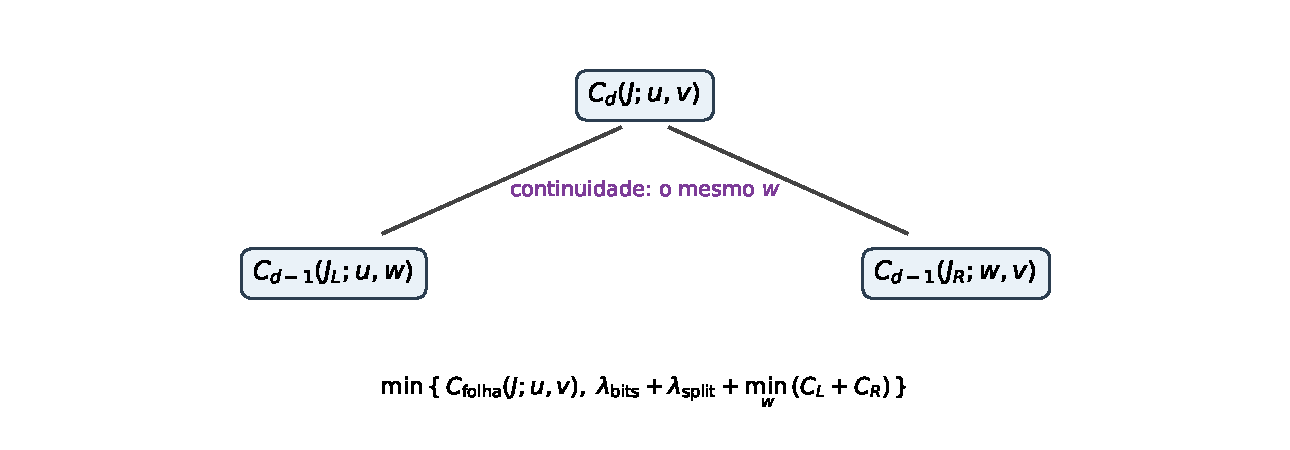
\includegraphics[width=.92\linewidth]{fig01_estado_fronteira.pdf}
 \caption{O estado registra os dois valores externos; o valor $w$ é
 compartilhado pelos filhos e impõe continuidade. O termo de subdivisão
 inclui o bit do nó interno e a penalidade estrutural.}
 \label{fig:boundary-state}
\end{figure}

\begin{theorem}[correção para árvore fixa]
\label{thm:fixed-correctness}
Para todo nó $J$ de $T$ e todo par de estados $(u,v)$,
\begin{equation}
 C_T(J;u,v)
 =\min_{R\in\Representations_H(T_J;u,v)}
 \cost_{\mathcal Z}(R),
 \label{eq:fixed-correctness}
\end{equation}
com valor $+\infty$ se o conjunto à direita for vazio. Se, em cada mínimo,
for armazenado também o candidato de menor chave \eqref{eq:tie-key}, a
retropropagação reconstrói uma única representação canônica. Em particular,
\begin{equation}
 \min_{u,v\in\Values_{D,H}(K)}C_T(K;u,v)
 =\min_{R\in\Representations_H(T)}\cost_{\mathcal Z}(R).
 \label{eq:fixed-global}
\end{equation}
\end{theorem}

\begin{proof}
Proceda por indução na altura da subárvore. Se $J$ é folha, a
\cref{prop:endpoint-dictionary} mostra que existe exatamente um rótulo com
fronteiras $(u,v)$ quando $(u,v)\in\Pairs_H(J)$, e nenhum nos demais casos.
Seu custo é precisamente \eqref{eq:leaf-cost}, provando
\eqref{eq:fixed-leaf}.

Suponha agora que $J$ tenha filhos. Toda montagem contínua em $T_J$ possui um
único valor $w$ na fronteira compartilhada. Sua restrição aos filhos pertence
a
\[
 \Representations_H(T_{J_L};u,w)
 \quad\text{e}\quad
 \Representations_H(T_{J_R};w,v).
\]
Reciprocamente, quaisquer duas representações desses conjuntos colam-se em
uma representação contínua de $T_J$. Pelo \cref{lem:recursive-stream}, a
colagem acrescenta um bit de nó interno; ela também acrescenta uma
subdivisão. A aditividade da perda e das duas penalidades dá
\eqref{eq:fixed-split}. Aplicar a hipótese de indução aos dois filhos prova
\eqref{eq:fixed-correctness}.

Há um número finito de estados e candidatos. A ordem de
\eqref{eq:tie-key} é total e, pelo \cref{lem:tie-concatenation}, guardar o
menor candidato em cada estado não elimina o minimizador canônico de nenhuma
superárvore. Os apontadores dos valores $w$ e das decisões recuperam esse
candidato. Minimizar também sobre os dois valores externos da raiz prova
\eqref{eq:fixed-global}.
\end{proof}

\begin{algorithm}[rotulação exata de uma árvore fixa]
\label{alg:fixed-tree}
Enumere $\Pairs_H(J)$ em cada folha. Percorra $T$ em pós-ordem. Em cada nó
interno, agrupe os estados do filho direito pelo valor de fronteira esquerdo
$w$ e una apenas pares com o mesmo $w$. Para cada estado externo $(u,v)$,
retenha a menor chave \eqref{eq:tie-key} e um apontador para os dois filhos.
Na raiz, escolha a menor entrada finita e siga os apontadores.
\end{algorithm}

O agrupamento por $w$ não altera a recorrência; ele apenas evita testar pares
de subárvores que violam continuidade de maneira evidente.

\section{Seleção simultânea da árvore e dos átomos}
\label{sec:variable-dp}

Para uma célula $J$ e um inteiro $d\ge0$, seja
\[
 \Representations_{d,H}(J;u,v)
\]
o conjunto das representações contínuas enraizadas em $J$, com profundidade
relativa no máximo $d$, folhas rotuladas por $\Library_H$ e valores externos
$u,v$. Diferentemente da seção anterior, a forma da árvore não é fixada.

A recorrência usa o princípio de otimalidade de \citet{bellman1957}. A
aproximação de curvas por segmentos via programação dinâmica já aparece em
\citet{bellman1961}, com antecedentes para segmentos lineares em
\citet{stone1961} e desenvolvimentos posteriores para aproximação poligonal
ótima em \citet{perezvidal1994}; aqui o estado contém os dois valores de
fronteira e a decisão de manter ou subdividir uma célula diádica.

\begin{definition}[recorrência de Bellman com árvore variável]
\label{def:variable-recurrence}
Para $d=0$, ponha
\begin{equation}
 C_0(J;u,v)=\Phi_H(J;u,v).
 \label{eq:variable-base}
\end{equation}
Para $d\ge1$, se $J_L,J_R$ são os filhos de $J$, defina
\begin{align}
 C_d(J;u,v)
 =\min\Bigl\{&
 \Phi_H(J;u,v),\notag\\
 &\lambda_{\rm bits}+\lambda_{\rm split}
 +\min_{w\in\Values_{D,H}(K)}
 \bigl[C_{d-1}(J_L;u,w)+C_{d-1}(J_R;w,v)\bigr]
 \Bigr\}.
 \label{eq:variable-recurrence}
\end{align}
\end{definition}

O primeiro ramo mantém $J$ como folha; o segundo subdivide, escolhe o valor
racional intermediário e reutiliza os ótimos dos dois filhos. A profundidade
global $D$ é usada somente para fixar um alfabeto comum suficientemente
grande; na chamada em $J$, $d$ é o número de níveis ainda disponíveis.

\begin{theorem}[exatidão, existência e determinismo]
\label{thm:variable-correctness}
Seja $J$ uma célula descendente de $K$ na profundidade relativa $r$. Para todo
$d\le D-r$ e todo $(u,v)\in\Values_{D,H}(K)^2$,
\begin{equation}
 C_d(J;u,v)
 =\min_{R\in\Representations_{d,H}(J;u,v)}
 \cost_{\mathcal Z}(R).
 \label{eq:variable-correctness}
\end{equation}
Consequentemente,
\begin{equation}
 C_{D,H}^{\star}(K)
 :=\min_{u,v\in\Values_{D,H}(K)}C_D(K;u,v)
 =\min_{R\in\Representations_{D,H}^{\Library}(K)}
 \cost_{\mathcal Z}(R).
 \label{eq:variable-global}
\end{equation}
O mínimo é finito quando
$H\ge\max\{2,k_0+1,|m_0|+1\}$. Com o desempate
\eqref{eq:tie-key}, o algoritmo devolve uma única representação, independentemente
da ordem em que estados, átomos ou valores intermediários sejam gerados.
\end{theorem}

\begin{proof}
A prova é por indução em $d$. Para $d=0$, apenas a árvore-folha é permitida,
e \eqref{eq:variable-base} coincide com seu custo ou vale $+\infty$ quando o
par é inadmissível.

Suponha o resultado para $d-1$. Toda representação de profundidade no máximo
$d$ está em exatamente um de dois casos: a raiz é folha; ou a raiz é interna
e possui duas subárvores de profundidade no máximo $d-1$. No segundo caso, a
continuidade produz um único valor compartilhado $w$. Reciprocamente, a
colagem de quaisquer duas subárvores com o mesmo $w$ é admissível. A
decomposição do custo é a mesma do \cref{thm:fixed-correctness}; portanto a
partição exaustiva dos candidatos nos dois casos é exatamente
\eqref{eq:variable-recurrence}. A hipótese de indução completa
\eqref{eq:variable-correctness}.

Minimizar os estados externos na raiz prova \eqref{eq:variable-global}. Sob a
hipótese sobre $H$, o átomo de parâmetros $(k_0,m_0,0,1)$ pertence a
$\Library_H$, logo o catálogo contém ao menos a árvore-folha e o mínimo é
finito. Todos os conjuntos examinados são finitos. A chave
\eqref{eq:tie-key} é total e depende somente do candidato, não da ordem de
geração, o que prova o determinismo.
\end{proof}

\begin{corollary}[compatibilidade com a enumeração de formas]
\label{cor:shape-enumeration}
Se $\Trees_D(K)$ é o conjunto finito de todas as formas de árvore de
profundidade no máximo $D$, então
\begin{equation}
 C_{D,H}^{\star}(K)
 =\min_{T\in\Trees_D(K)}
   \min_{u,v\in\Values_{D,H}(K)}C_T(K;u,v).
 \label{eq:shape-equivalence}
\end{equation}
O mesmo fluxo canônico vence nos dois lados.
\end{corollary}

\begin{proof}
As classes $\Representations_H(T)$, $T\in\Trees_D(K)$, particionam as
representações pela forma da árvore. Aplique os
\cref{thm:fixed-correctness,thm:variable-correctness} e o mesmo desempate
total.
\end{proof}

\begin{algorithm}[seletor exato por programação dinâmica]
\label{alg:variable-tree}
Construa as tabelas em pós-ordem na árvore diádica completa de profundidade
$D$. Inicialize cada estado com o candidato folha, quando admissível. Una as
tabelas dos filhos pelo valor intermediário $w$, acrescente o marcador e a
penalidade de subdivisão e substitua a entrada somente quando a chave completa
diminuir. A tabela da raiz e os apontadores guardados fornecem o ótimo global
e sua representação.
\end{algorithm}

\section{Orçamentos rígidos e erro uniforme}
\label{sec:hard-budgets}

Além do funcional penalizado, um orçamento explícito de folhas pode ser
incorporado ao estado sem alterar o princípio de otimalidade.

\subsection{Número exato de folhas}

Para $1\le n\le2^d$, defina $C_{d,n}(J;u,v)$ como o menor valor de
\eqref{eq:additive-objective} entre representações com exatamente $n$ folhas.
A recorrência é
\begin{align}
 C_{0,1}(J;u,v)&=\Phi_H(J;u,v),\label{eq:budget-base}\\
 C_{0,n}(J;u,v)&=+\infty,\qquad n>1,\notag\\
 C_{d,1}(J;u,v)&=\Phi_H(J;u,v),\qquad d\ge1,\label{eq:budget-one}\\
 C_{d,n}(J;u,v)&=\lambda_{\rm bits}+\lambda_{\rm split}\notag\\
 &\quad+\min_{\substack{n_L+n_R=n\\n_L,n_R\ge1}}
 \min_{w\in\Values_{D,H}(K)}
 \{C_{d-1,n_L}(J_L;u,w)+C_{d-1,n_R}(J_R;w,v)\},
 \quad n\ge2.
 \label{eq:budget-recurrence}
\end{align}

\begin{theorem}[correção sob orçamento de folhas]
\label{thm:leaf-budget}
As recorrências \eqref{eq:budget-base}--\eqref{eq:budget-recurrence}
calculam exatamente o menor custo entre representações de profundidade no
máximo $d$, altura no máximo $H$, fronteiras $(u,v)$ e exatamente $n$
folhas. Em particular, o ótimo com no máximo $N$ folhas é
\begin{equation}
 \min_{\substack{1\le n\le\min\{N,2^D\}\\
                  u,v\in\Values_{D,H}(K)}}
 C_{D,n}(K;u,v).
 \label{eq:at-most-N}
\end{equation}
\end{theorem}

\begin{proof}
A indução em $d$ é idêntica à do
\cref{thm:variable-correctness}, com uma coordenada adicional. Uma
representação com uma folha usa o primeiro ramo. Se possui $n\ge2$ folhas,
sua raiz é interna e as quantidades positivas de folhas dos filhos satisfazem
$n_L+n_R=n$. Reciprocamente, toda escolha listada em
\eqref{eq:budget-recurrence} cola duas representações com exatamente $n$
folhas. A união sobre $1\le n\le N$ prova \eqref{eq:at-most-N}.
\end{proof}

\subsection{Recorrência de gargalo para a norma uniforme}

Seja agora $f\in C(K)$ e suponha disponível, para cada par admissível, o erro
local exato
\begin{equation}
 e_f(J;u,v)=\|f-\ell_{J;u,v}\|_{\infty,J}.
 \label{eq:local-uniform-error}
\end{equation}
Quando o par é inadmissível, ponha $e_f=+\infty$. Não se supõe que esse oráculo
exista para toda apresentação de uma função contínua; para polinômios e
famílias elementares ele pode ser produzido por cálculo simbólico ou por
aritmética intervalar certificada.

Defina $B_{d,n}(J;u,v)$ substituindo soma de perdas pelo máximo entre folhas:
\begin{align}
 B_{0,1}(J;u,v)&=e_f(J;u,v),\label{eq:bottleneck-base}\\
 B_{0,n}(J;u,v)&=+\infty,\qquad n>1,\notag\\
 B_{d,1}(J;u,v)&=e_f(J;u,v),\label{eq:bottleneck-one}\\
 B_{d,n}(J;u,v)
 &=\min_{\substack{n_L+n_R=n\\n_L,n_R\ge1}}
 \min_{w\in\Values_{D,H}(K)}
 \max\{B_{d-1,n_L}(J_L;u,w),
       B_{d-1,n_R}(J_R;w,v)\}.
 \label{eq:bottleneck-recurrence}
\end{align}

Seja
\begin{equation}
 E_{N,H,D}^{\rm tree}(f)_\infty
 =\min\{\|f-\Eval(R)\|_{\infty,K}:
 R\in\Representations_{D,H}^{\Library}(K),\
 |\Lambda(R)|\le N\}.
 \label{eq:truncated-tree-error}
\end{equation}

\begin{theorem}[cálculo exato do melhor erro truncado]
\label{thm:bottleneck}
Sob o oráculo \eqref{eq:local-uniform-error},
\begin{equation}
 E_{N,H,D}^{\rm tree}(f)_\infty
 =\min_{\substack{1\le n\le\min\{N,2^D\}\\
                  u,v\in\Values_{D,H}(K)}}
 B_{D,n}(K;u,v).
 \label{eq:bottleneck-optimum}
\end{equation}
Se
\begin{equation}
 D\ge \max\{0,H-k_0-1\},
 \label{eq:depth-inactive}
\end{equation}
a restrição de profundidade já é inativa: nenhum átomo de $\Library_H$
apoiado em descendente de $K$ pode ocorrer abaixo desse nível.
\end{theorem}

\begin{proof}
Em uma montagem contínua, o erro uniforme global é o máximo dos erros nas
folhas. A mesma partição em raiz-folha ou raiz-interna usada no
\cref{thm:leaf-budget} produz
\eqref{eq:bottleneck-recurrence}, agora com o operador máximo na colagem.
A indução em $d$ prova que $B_{d,n}$ é o melhor gargalo com o estado e a
quantidade de folhas fixados. Minimizar essas coordenadas dá
\eqref{eq:bottleneck-optimum}.

Uma folha na profundidade relativa $r$ tem escala $k_0+r$. Pela altura
\eqref{eq:inherited-height}, sua admissibilidade exige
$k_0+r+1\le H$. Portanto $r\le H-k_0-1$, o que prova a última afirmação.
\end{proof}

\begin{remark}[interação entre profundidade e translação]
\label{rem:depth-vs-translation}
A condição \eqref{eq:depth-inactive} satura o ganho obtido pelo aumento de $D$
além de $H-k_0-1$. A admissibilidade de cada célula também depende de sua
posição.
Para $m_0\ge0$, a \cref{prop:translation-obstruction} mostra que o refinamento
uniforme completo exige também
$r\le\log_2\bigl(H/(m_0+1)\bigr)$. Quando esse segundo limiar é o menor, o
catálogo se torna espacialmente assimétrico antes de a escala se esgotar. Ao ler
\eqref{eq:bottleneck-optimum} para um dado $(N,H,D)$, portanto, o orçamento de
folhas $N$ compete com uma família de árvores que já está truncada pela
translação, não apenas pela profundidade.
\end{remark}

\begin{corollary}[convergência para funções contínuas]
\label{cor:uniform-convergence}
Para todo $f\in C(K)$,
\begin{equation}
 \inf_{N,H,D}E_{N,H,D}^{\rm tree}(f)_\infty=0.
 \label{eq:uniform-convergence}
\end{equation}
Mais precisamente, ao longo de qualquer sequência de triplas $(N,H,D)$ que
seja componente a componente não decrescente e cofinal, os erros convergem a
zero.
\end{corollary}

\begin{proof}
Os catálogos são aninhados em cada orçamento, logo os erros não crescem. O
teorema de densidade da \cref{sec:assemblies} afirma que, dado $\varepsilon>0$,
existe uma montagem contínua finita de átomos com erro menor que
$\varepsilon$. Essa representação possui números finitos de folhas,
profundidade e altura; portanto pertence a algum catálogo da união. Assim, o
ínfimo em \eqref{eq:uniform-convergence} é zero, e a monotonicidade prova a
convergência cofinal.
\end{proof}

\section{Complexidade, truncagem e estabilidade}
\label{sec:complexity-dp}

\subsection{Contagem de operações}

Escreva
\[
 M=|\Values_{D,H}(K)|,\qquad S_D=2^{D+1}-1.
\]
As cotas abaixo usam o modelo de custo unitário para operações e comparações
no corpo ordenado dos custos. O tamanho dos operandos racionais será discutido
separadamente. O custo do terceiro componente da chave \eqref{eq:tie-key}, o
\emph{fluxo binário completo}, é contado em bits. Comparar duas
chaves que empatam nas duas primeiras componentes custa
$O(L)$, onde
\begin{equation}
 L=\max_R|\ser_{\rm rec}(R)|
 \le S_D\bigl(2\lfloor\log_2|\Library_H|\rfloor+2\bigr)
 \label{eq:stream-length}
\end{equation}
é o comprimento máximo de fluxo no catálogo. Todas as cotas desta seção contam
comparações de chave e construção/concatenação de fluxos como unitárias;
multiplicá-las por $L$ dá uma cota superior correspondente no modelo em que
comparar ou copiar um bit tem custo unitário.
Pela mesma razão, as cotas de memória contam \emph{entradas} da tabela, e cada
entrada que armazena um fluxo ocupa até $L$ bits. Uma implementação que
guarde apenas ponteiros de reconstrução e recomponha o fluxo sob demanda
troca esse fator de memória por trabalho adicional na comparação.

\begin{theorem}[complexidade em número de estados]
\label{thm:state-complexity}
Suponha os custos de folha pré-computados. Uma implementação densa do
\cref{alg:variable-tree} usa
\begin{equation}
 O(S_DM^3)
 \label{eq:dense-time}
\end{equation}
operações e
\begin{equation}
 O(S_DM^2)
 \label{eq:dense-memory}
\end{equation}
entradas de memória quando preserva todos os apontadores de reconstrução.
A versão com orçamento de até $N$ folhas usa
\begin{equation}
 O(S_DN^2M^3)
 \label{eq:budget-time}
\end{equation}
operações e $O(S_DNM^2)$ entradas. Se cada custo local
\eqref{eq:local-loss} for calculado diretamente sobre $P$ observações, a
inicialização densa acrescenta $O(S_DPM^2)$ operações.
\end{theorem}

\begin{proof}
Cada nó tem no máximo $M^2$ estados externos $(u,v)$. Em um nó interno, a
recorrência testa no máximo $M$ valores intermediários $w$ por estado, logo
$O(M^3)$ operações. Há no máximo $S_D$ nós. Armazenar um custo e um apontador
por estado dá \eqref{eq:dense-memory}.

Com o número de folhas no estado, há $N$ camadas de custo. Somando, para todos
$n\le N$, as decomposições positivas $n_L+n_R=n$, obtêm-se $O(N^2)$ pares de
orçamentos por tripla $(u,w,v)$. Isso prova \eqref{eq:budget-time} e a cota de
memória. A última afirmação vem de somar até $P$ termos em cada custo local.
\end{proof}

\begin{remark}[tabelas esparsas]
\label{rem:sparse}
As cotas são deliberadamente densas. O algoritmo distribuído armazena apenas
pares realizáveis e agrupa o filho direito por $w$. Seu trabalho em um nó é
proporcional ao tamanho da junção
\[
 \#\{((u,w),(w,v)):\text{os dois estados estão presentes}\},
\]
que pode ser muito menor que $M^3$. Essa melhora depende da instância e não
altera a cota de pior caso.

Convém dizer o quanto. Na instância principal da \cref{sec:numerical}, com
$(D,H)=(3,4)$, o alfabeto efetivo tem $M=475$ elementos, contra
$2S_Dq_H(q_H-1)=15\,180$ pela primeira cota de
\eqref{eq:value-alphabet-bound} e $36H^6=147\,456$ pela segunda; e a tabela da
raiz contém $3\,383$ estados realizáveis, contra $M^2=225\,625$ posições
densas, isto é, uma ocupação de $1{,}5\%$. Nas instâncias examinadas, a
estrutura esparsa reduz substancialmente o trabalho em relação à cota densa de
pior caso.
\end{remark}

\subsection{Modelo de custo e complexidade de bits}

Pelo \cref{lem:value-alphabet},
\[
 M\le36H^6,
\]
e portanto \eqref{eq:dense-time} fornece, de modo bruto,
\begin{equation}
 O(S_DH^{18})
 \label{eq:height-worst}
\end{equation}
operações de custo unitário. A expressão é polinomial no valor numérico de
$H$, cujo comprimento binário é $O(\log H)$, e
$S_D=2^{D+1}-1$. Trata-se, portanto, de uma cota pseudo-polinomial nos
orçamentos codificados em binário.

Para fechar também esse segundo nível, defina, para $r=p/q$ reduzido, $q>0$,
\begin{equation}
 \operatorname{bl}(r)
 :=1+\left\lceil\log_2(|p|+1)\right\rceil
    +\left\lceil\log_2(q+1)\right\rceil .
 \label{eq:rational-bit-length}
\end{equation}
Seja $B_{\mathcal Z}$ o maior comprimento \eqref{eq:rational-bit-length}
entre abscissas, respostas, pesos e penalidades racionais da instância. Denote
por $\mathsf M_{\mathbb Z}(b)$ uma cota para multiplicar inteiros de $b$ bits,
e recorde o limite $L$ de \eqref{eq:stream-length}.

\begin{theorem}[cota grosseira de complexidade de bits]
\label{thm:bit-complexity}
Todos os custos racionais que aparecem na recorrência possuem numeradores e
denominadores de comprimento no máximo
\begin{equation}
 B_{\rm cost}
 =O\!\left(
 P\bigl(B_{\mathcal Z}+D+|k_0|+\log(2H)\bigr)
 +B_{\mathcal Z}+D+\log(2L)
 \right).
 \label{eq:cost-bit-growth}
\end{equation}
Consequentemente, a versão densa sem orçamento de folhas pode ser executada em
\begin{equation}
 O\!\left(
 (S_DM^3+S_DPM^2)
 \bigl[\mathsf M_{\mathbb Z}(B_{\rm cost})
       \log(2B_{\rm cost})+L\bigr]
 \right)
 \label{eq:dense-bit-time}
\end{equation}
operações de bit e
\begin{equation}
 O\!\left(S_DM^2(B_{\rm cost}+L)\right)
 \label{eq:dense-bit-memory}
\end{equation}
bits de memória quando todos os estados e fluxos são armazenados. Na versão
com até $N$ folhas, substituem-se $S_DM^3$ e $S_DM^2$ por
$S_DN^2M^3$ e $S_DNM^2$, respectivamente. Com multiplicação escolar,
$\mathsf M_{\mathbb Z}(b)=O(b^2)$.
\end{theorem}

\begin{proof}
Um átomo admissível tem $\operatorname{bl}(y_0),
\operatorname{bl}(s)=O(\log(2H))$. Em uma célula descendente de profundidade
no máximo $D$, escrever o centro ou um extremo como racional expande o fator
diádico em no máximo $D+|k_0|+O(1)$ bits. Portanto a avaliação afim em uma
abscissa da amostra tem comprimento
\[
 O(B_{\mathcal Z}+D+|k_0|+\log(2H)).
\]
Subtrair a resposta, elevar ao quadrado e multiplicar pelo peso apenas altera
a constante dessa cota. Na soma ingênua de $P$ frações, pode-se tomar como
denominador o produto dos denominadores; logo numerador e denominador têm
comprimento no máximo $P$ vezes o maior comprimento de uma parcela. Os termos
de penalização acrescentam $O(B_{\mathcal Z}+D+\log(2L))$ bits. Isso prova
\eqref{eq:cost-bit-growth}; cancelamentos por máximo divisor comum só podem
reduzir os operandos.

Uma soma, comparação ou redução de frações com operandos de comprimento
$B_{\rm cost}$ custa
$O(\mathsf M_{\mathbb Z}(B_{\rm cost})\log(2B_{\rm cost}))$ operações de bit
por algoritmos inteiros usuais. Quando custos e número de folhas empatam, a
comparação shortlex lê no máximo $L$ bits. Multiplicar esse custo pelo número
de transições e inicializações do \cref{thm:state-complexity} dá
\eqref{eq:dense-bit-time}. Cada estado guarda um custo, um fluxo ou apontador
de reconstrução e índices de $O(\log(S_DM))$ bits, absorvidos pela cota exibida;
isso prova \eqref{eq:dense-bit-memory}. O argumento com a coordenada de
orçamento é idêntico.
\end{proof}

A cota é propositalmente conservadora: ela não explora cancelamentos nem
denominadores compartilhados. Ainda assim, fecha o modelo de Turing e torna
explícito o ponto essencial. Como $M\le36H^6$ e $S_D=2^{D+1}-1$, a
dependência continua pseudo-polinomial nos valores numéricos de $H$ e $2^D$,
mesmo após contabilizar o crescimento dos racionais.

\subsection{Valores sob truncagem}

Seja
\[
 \Representations_{\infty}^{\Library}(K)
 =\bigcup_{D,H}\Representations_{D,H}^{\Library}(K)
\]
o conjunto de todas as representações finitas enraizadas em $K$.

\begin{proposition}[convergência dos mínimos penalizados]
\label{prop:truncation-convergence}
Os valores $C_{D,H}^{\star}(K)$ de \eqref{eq:variable-global} são não
crescentes separadamente em $D$ e $H$, e
\begin{equation}
 \inf_{D,H}C_{D,H}^{\star}(K)
 =\inf_{R\in\Representations_{\infty}^{\Library}(K)}
   \cost_{\mathcal Z}(R).
 \label{eq:penalized-limit}
\end{equation}
Ao longo de qualquer sequência componente a componente não decrescente e
cofinal em $(D,H)$, os valores convergem ao lado direito.

Se o ínfimo em \eqref{eq:penalized-limit} é atingido, o minimizador global de
menor chave \eqref{eq:tie-key} pertence a algum catálogo finito; a partir de
uma truncagem que o contenha, o seletor canônico estabiliza.
\end{proposition}

\begin{proof}
Aumentar $D$ ou $H$ preserva toda representação já admissível, logo os
mínimos não crescem. A união dos domínios dos mínimos é exatamente
$\Representations_{\infty}^{\Library}(K)$, o que prova
\eqref{eq:penalized-limit}. Uma sequência cofinal eventualmente contém cada
representação finita; a monotonicidade conclui a convergência.

Se há minimizadores globais, seus comprimentos de fluxo formam um subconjunto
não vazio de $\Nzero$ e possuem mínimo. Entre as finitíssimas palavras desse
comprimento existe uma menor lexicograficamente. A representação
correspondente tem profundidade e altura finitas. Depois que ela entra no
catálogo, nenhum candidato posterior pode melhorar o custo ou a chave.
\end{proof}

\subsection{Um limite de estabilidade}

\begin{proposition}[um seletor exato pode ser descontínuo]
\label{prop:instability}
Considere, em $K=[0,1]$, o subcatálogo formado pelos dois átomos
\[
 g_+(x)=x,\qquad g_-(x)=-x,
\]
ambos de altura $2$. Para uma única observação $(x,z)=(1,z)$, custo igual à
perda quadrática e qualquer desempate determinístico, o mapa que envia $z$ ao
átomo selecionado é descontínuo em $z=0$ na norma uniforme.
\end{proposition}

\begin{proof}
Os custos são
\[
 \cost_z(g_+)=(z-1)^2,\qquad
 \cost_z(g_-)=(z+1)^2.
\]
Logo $g_+$ é o único minimizador para $z>0$, $g_-$ é o único minimizador para
$z<0$ e há empate em $z=0$. Qualquer regra escolhe um deles no empate, mas a
sequência que se aproxima por dados do lado oposto seleciona sempre o outro.
Como
\[
 \|g_+-g_-\|_{\infty,[0,1]}=2,
\]
não há continuidade.
\end{proof}

O exemplo separa exatidão de continuidade do seletor. Hipóteses de margem
entre custos produzem regiões de seleção localmente constante; nos empates,
uma saída a valores conjuntos preserva semicontinuidade. Essa distinção entre
existência, estabilidade e não unicidade também aparece na análise de problemas
de treinamento por perda quadrática em esquemas não lineares
\citep{christof2021}.

\section{Validação computacional exata}
\label{sec:numerical}

\subsection{Implementação}

O script
\path{reproducibility/selecao/seletor_dinamico_exato.py}
implementa os \cref{alg:fixed-tree,alg:variable-tree}. O domínio numérico é
\texttt{Fraction}. As tabelas são dicionários esparsos indexados
por pares de \texttt{Fraction}; a junção dos filhos usa igualdade racional
exata no valor $w$. Perdas, penalidades, comparações de objetivo, alturas,
endereços $\Gamma^\sharp$ e desempates não usam ponto flutuante.
\texttt{NumPy} e \texttt{Matplotlib} aparecem somente depois da seleção, para
desenhar as figuras.

Cada execução verifica:
\begin{enumerate}[label=(\alph*),leftmargin=2em]
 \item a continuidade de todas as fronteiras da montagem vencedora;
 \item a altura de cada folha;
 \item a igualdade entre o ótimo da recorrência variável e o mínimo obtido ao
 enumerar separadamente todas as formas e resolver cada árvore fixa;
 \item a coincidência com uma enumeração direta de representações na
 instância mínima descrita abaixo;
 \item que uma derivação separada de $\mathcal Q_H$, dos pares de extremos
 e das perdas locais coincide com as rotinas usadas pela PD;
 \item as recorrências com número exato de folhas e de gargalo contra
 enumeração sem poda;
 \item a robustez da comparação num orçamento sem células eliminadas;
 \item que o valor exato não excede os valores das três referências.
\end{enumerate}

O verificador de (d) é independente da \emph{recorrência}, mas reutiliza o
catálogo local e a função de perda. Por isso (e) constitui uma segunda camada:
ela enumera $\mathcal Q_H$ diretamente pelas frações reduzidas, forma os pares
de extremos a partir de $(y_0,s)$ sem chamar o dicionário da PD e recompõe
\eqref{eq:local-loss} pela fórmula afim nos pontos observados. As duas
comparações possuem, assim, implementações independentes do dicionário e da
perda. O teste de erro uniforme em (f) usa $f\equiv0$, caso em que
$e_f(J;u,v)=\max\{|u|,|v|\}$ é calculado exatamente.

\subsection{Auditoria por enumeração direta}

Na instância de auditoria, tomam-se $(D,H)=(1,2)$, as cinco observações
racionais $x_i\in\{0,\tfrac14,\tfrac12,\tfrac34,1\}$ do alvo $2|x-1/2|$ e as
penalidades $\lambda_{\rm bits}=\tfrac1{200}$,
$\lambda_{\rm split}=\tfrac1{50}$. Há $42$ átomos admissíveis na
raiz. O verificador examina diretamente os $42$ candidatos de uma folha e
todos os $42^2=1764$ pares de átomos dos filhos, descartando os $1704$ pares
que não coincidem em $x=1/2$. Restam $60$ subdivisões contínuas, ou $102$
representações ao contar também as folhas. O custo e o fluxo vencedores
coincidem bit a bit com a programação dinâmica.

Nessa instância, como na instância principal, o minimizador de custo é único,
de modo que ela não chega a exercitar o desempate \eqref{eq:tie-key}. O script
inclui por isso três cenários dedicados, nos quais o vencedor da recorrência é
confrontado com a minimização exaustiva da chave completa sobre todas as
representações contínuas, enumeradas \emph{sem} poda por estado:
\begin{enumerate}[label=(\alph*),leftmargin=2em]
 \item com dados e penalidades nulos e $(D,H)=(1,2)$, todas as $102$
 representações têm custo zero e a seleção é decidida pelo comprimento do
 fluxo;
 \item o mesmo com $(D,H)=(2,3)$, em que as $1370$ representações contínuas
 empatam em custo, o que exercita dois níveis de concatenação;
 \item com dados identicamente nulos e $(D,H)=(2,3)$, dois candidatos empatam
 simultaneamente em custo e em comprimento, e a seleção é decidida pela ordem
 lexicográfica do fluxo.
\end{enumerate}
Nos três casos a recorrência devolve exatamente o mesmo fluxo que a
minimização exaustiva, o que verifica a compatibilidade de \eqref{eq:tie-key}
com a concatenação afirmada no \cref{thm:fixed-correctness}.

Para testar a \cref{sec:hard-budgets}, o script enumera sem poda todas as
$1370$ representações contínuas de $(D,H)=(2,3)$. Para cada número viável de
folhas e cada par de estados externos, compara tanto o melhor custo aditivo
$C_{d,n}$ quanto o melhor gargalo $B_{d,n}$ com a enumeração completa. Também
compara, para cada $N\in\{1,2,3,4\}$, o ótimo com no máximo $N$ folhas. Todas
as igualdades são verificadas em aritmética racional exata.

\begin{table}[t]
 \centering
 \caption{Verificações executáveis das duas instâncias.}
 \label{tab:dp-audit}
 \small
 \begin{tabularx}{\linewidth}{@{}Xr@{}}
\toprule
Verificação & resultado \\
\midrule
Dicionário/perdas derivados das definições & true \\
Enumeração direta $(D,H)=(1,2)$ & true \\
Pares de subárvores examinados diretamente & 1764 \\
Formas de árvore enumeradas na instância principal & 26 \\
Formas de árvore com catálogo não vazio & 11 \\
Células da árvore completa sem átomo admissível & 4 \\
DP variável $=$ mínimo sobre formas fixas & true \\
Empates de custo máximos resolvidos pela chave & 1370 \\
DP $=$ mínimo exaustivo sob empate & true \\
Fórmula geométrica (1350 casos) & true \\
Orçamento de folhas $=$ enumeração exaustiva & true \\
Gargalo uniforme $=$ enumeração exaustiva & true \\
Ótimo exato não pior que as três referências & true \\
\bottomrule
\end{tabularx}

\end{table}

As contagens e os fluxos da \cref{tab:dp-audit} coincidem com a enumeração
exaustiva independente em todas as instâncias indicadas, inclusive para a
recorrência de gargalo do \cref{thm:bottleneck}.

\subsection{Instância de regressão e rotas de controle}

O experimento a seguir é uma regressão interna de correção, não um estudo de
desempenho nem uma comparação empírica de métodos. As três rotas auxiliares
servem somente como candidatos admissíveis cujo custo exato deve ser maior ou
igual ao ótimo da programação dinâmica. Não se inferem velocidade, qualidade
estatística ou superioridade prática a partir desta única instância sintética.

A instância principal usa $K=[0,1]$, $(D,H)=(3,4)$ e as $17$ observações
diádicas $x_i=i/16$ do alvo racional
\begin{equation}
 f(x)=\frac{1}{1+16(x-\tfrac14)^2}.
 \label{eq:experiment-target}
\end{equation}
As penalidades são
\[
 \lambda_{\rm bits}=\frac1{500},
 \qquad
 \lambda_{\rm split}=\frac1{100}.
\]
Há $23$ valores racionais e $22$ inclinações não nulas de altura no máximo
$4$, isto é, $506$ átomos por célula geometricamente admissível. A árvore
completa possui $15$ células, das quais $11$ são admissíveis: pela
\cref{prop:translation-obstruction}, as quatro células de profundidade $3$ que
cobrem $[\tfrac12,1]$ têm $m\in\{4,5,6,7\}$ e nenhum átomo de altura no
máximo $4$. Consequentemente, das $26$ formas de árvore de profundidade no
máximo $3$, apenas $11$ admitem alguma rotulação contínua; as $15$ restantes
--- todas as que subdividem a metade direita até a profundidade $3$ --- têm
catálogo vazio. As $26$ formas são enumeradas para auditoria, e o mínimo sobre
as viáveis coincide com a recorrência variável. A tabela esparsa da raiz
contém $3383$ estados realizáveis.

Essa assimetria deve ser mantida em vista ao ler a tabela: nesta instância a
metade esquerda do domínio é refinável até a profundidade $3$ e a metade
direita apenas até a profundidade $2$.

As rotas de controle são definidas sob o mesmo funcional:
\begin{itemize}[leftmargin=1.7em]
 \item \emph{malha uniforme}: escolhe o melhor entre as árvores completas de
 profundidades $0,1,2,3$, rotulando cada uma exatamente. Nesta instância a
 profundidade $3$ é \emph{inviável} --- sua metade direita não admite
 rotulação alguma ---, de modo que a escolha se dá de fato entre as
 profundidades $0$, $1$ e $2$, com objetivos $0{,}565803$, $0{,}572135$ e
 $0{,}376159$; vence a profundidade $2$, com quatro folhas;
 \item \emph{adaptativo certificado}: subdivide quando
 $M(J)|J|^2/8>\varepsilon_I$ e depois rotula a árvore exatamente; para
 \eqref{eq:experiment-target},
 \[
 f''(x)=
 \frac{32\bigl(48(x-\tfrac14)^2-1\bigr)}
      {\bigl(1+16(x-\tfrac14)^2\bigr)^3},
 \]
 e o máximo local é calculado racionalmente nos pontos críticos. O programa
 percorre $\varepsilon_I\in\{2^{-1},\dots,2^{-10}\}$ e retém o melhor
 resultado sob o mesmo objetivo da regressão; o caso retido é
 $\varepsilon_I=\tfrac12$. Registre-se que esse ajuste favorece a referência,
 e que apertar o certificado não ajuda: $\varepsilon_I\in\{2^{-3},2^{-4}\}$
 produz seis folhas e objetivo $0{,}571837$, e $\varepsilon_I\le2^{-5}$ exige
 uma árvore fora do catálogo;
 \item \emph{guloso}: começa na raiz, testa cada subdivisão de uma única folha,
 reotimiza exatamente todos os rótulos da árvore candidata e aceita apenas
 uma redução imediata do objetivo.
\end{itemize}

\begin{table}[t]
 \centering
 \caption{Regressão sob o mesmo custo racional. Os decimais arredondam a seis
 casas as frações brutas dos campos \texttt{loss\_exact} e
 \texttt{cost\_exact} do arquivo suplementar \texttt{resultados.json}.
 ``Erro quadrático'' é a soma ponderada dos resíduos quadráticos, não a sua
 média; a tabela não constitui um benchmark de desempenho.}
 \label{tab:selector-comparison}
 \small
 \begin{tabular}{lrrrr}
\toprule
Método & folhas & erro quadrático & bits & objetivo \\
\midrule
Ótimo exato & 3 & 0.041497 & 84 & 0.229497 \\
Malha uniforme & 4 & 0.116159 & 115 & 0.376159 \\
Adaptativo certificado & 3 & 0.041497 & 84 & 0.229497 \\
Heurística gulosa & 1 & 0.517803 & 24 & 0.565803 \\
\bottomrule
\end{tabular}

\end{table}

As frações brutas mencionadas na legenda estão no arquivo
\texttt{resultados.json}, no diretório \texttt{reproducibility/selecao}.

O ótimo exato possui três folhas:
\[
 [0,\tfrac14],\qquad[\tfrac14,\tfrac12],\qquad[\tfrac12,1],
\]
com valores nodais
\[
 \frac12,\quad1,\quad\frac12,\quad0.
\]
Suas inclinações são $2,-2,-1$ e sua altura máxima é $4$. O refinamento
certificado com $\varepsilon_I=\tfrac12$ coincide com essa árvore nesta
instância. A coincidência é registrada como propriedade deste caso de teste.
A melhor malha uniforme viável usa quatro folhas e tem
custo maior. A heurística gulosa permanece na raiz: a única subdivisão isolada
disponível eleva o objetivo de $0{,}565803$ para $0{,}572135$, embora duas
subdivisões coordenadas o reduzam para $0{,}229497$. O exemplo torna
visível a razão algorítmica para preservar estados e subproblemas em vez de
tomar apenas decisões locais.

\begin{figure}[t]
 \centering
 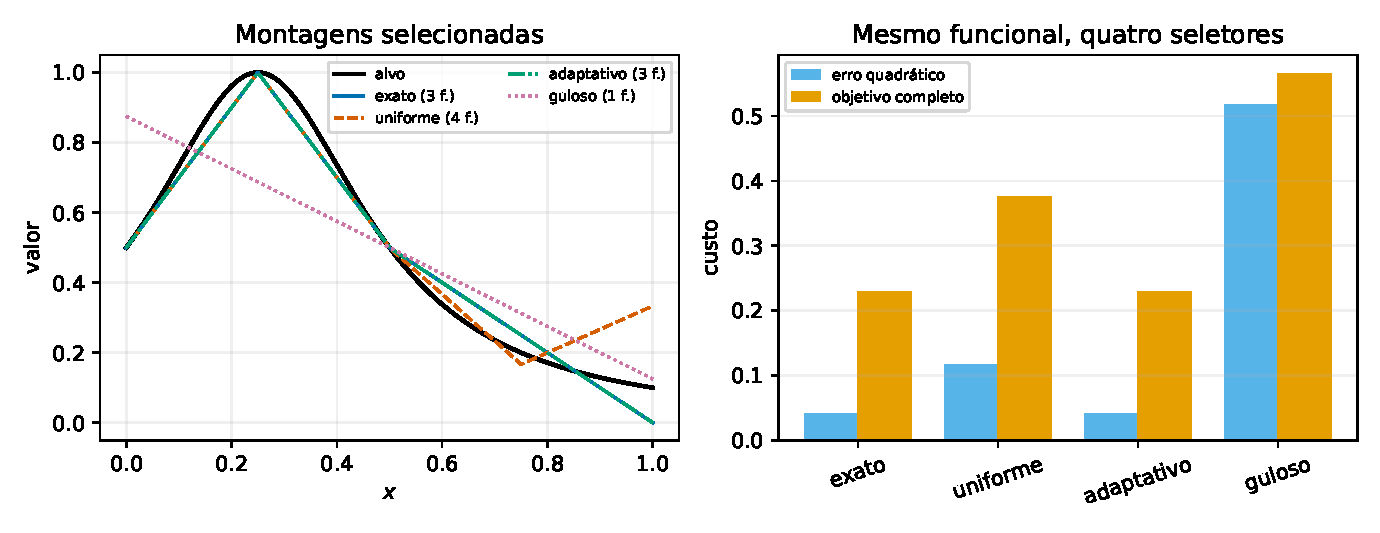
\includegraphics[width=\linewidth]{fig02_comparacao_seletores.pdf}
 \caption{À esquerda, o alvo e as quatro montagens. À direita, erro
 quadrático e objetivo completo. Todas as decisões foram tomadas com
 racionais exatos; o ponto flutuante é usado somente no desenho. A figura é
 um diagnóstico de regressão, não uma comparação de eficiência.}
 \label{fig:selector-comparison}
\end{figure}

O resultado visual da regressão aparece na
\cref{fig:selector-comparison}; os valores exatos correspondentes estão na
\cref{tab:selector-comparison}.

\subsection{Propriedades verificadas}

A regressão verifica três propriedades: o algoritmo realiza o mínimo do
catálogo declarado; reutiliza ótimos parciais em subproblemas repetidos; e
permanece estritamente abaixo de um candidato guloso específico quando a
melhora, nessa instância, requer decisões coordenadas. A terceira observação é
um teste de caso, não uma conclusão comparativa geral.

\subsection{Robustez sob truncagem do catálogo}
\label{sec:robustness}

Na instância $(D,H)=(3,4)$, a geometria do catálogo admite $11$ árvores e
elimina a malha uniforme mais fina. Para isolar esse efeito, tome
$(D,H)=(2,4)$, que satisfaz as duas
condições da \cref{prop:translation-obstruction} --- $k_0+D+1\le H$ e
$2^D(m_0+1)\le H$ ---, de modo que a árvore completa é integralmente
admissível: nenhuma célula é vazia e as cinco formas de profundidade no máximo
$2$ são viáveis. Com o mesmo alvo e as mesmas penalidades, as quatro rotas
produzem
\[
 0{,}229497,\quad 0{,}376159,\quad 0{,}229497,\quad 0{,}565803,
\]
com $3$, $4$, $3$ e $1$ folhas: exatamente os valores da
\cref{tab:selector-comparison}. O ótimo exato coincide, inclusive no fluxo
binário, com o da instância truncada --- o que era de esperar, pois suas três
folhas $[0,\tfrac14]$, $[\tfrac14,\tfrac12]$, $[\tfrac12,1]$ nunca descem
abaixo da profundidade $2$.

A truncagem por translação exclui corretamente a malha uniforme de
profundidade $3$, enquanto preserva o ótimo e seu fluxo binário. Em ambas as
instâncias, a rota gulosa implementada permanece presa na raiz; essa igualdade
de regressão não é extrapolada para outras heurísticas, dados ou regimes de
orçamento.

\part*{Constantes diádicas, estratos de altura e reversibilidade}
\addcontentsline{toc}{part}{Constantes diádicas, estratos de altura e reversibilidade}

Encerra-se aqui a teoria auxiliar de seleção exata. As seções seguintes
retomam a linha principal do documento-sistema: a constante assintótica da
interpolação estritamente diádica, os estratos de aproximação sob uma agenda
de altura aritmética e a caracterização direta e inversa. Elas não dependem
das recorrências de programação dinâmica e, na arquitetura editorial
congelada, pertencem às peças A e C, não ao residual R.

\section{Erro interpolatório ótimo em árvores estritamente diádicas}
\label{sec:dyadic-asymptotic}

Fixe primeiro o objeto cuja constante será determinada. Para uma célula
diádica $J=[a,b]$ e $f\in C(J)$, denote por $P_Jf$ a reta que interpola
$f(a)$ e $f(b)$ e ponha
\begin{equation}
 e_f(J)=\|f-P_Jf\|_{\infty,J}.
 \label{eq:local-interpolation-error}
\end{equation}
Se $\Lambda$ é o conjunto de folhas de uma árvore diádica finita com raiz
$K$, as retas $P_Jf$, $J\in\Lambda$, concordam nos nós compartilhados e
definem o interpolante contínuo $P_\Lambda f$. Defina
\begin{equation}
 E_N^{\rm dia}(f)_\infty
 =\min_{\substack{\Lambda\text{ árvore diádica}\\ |\Lambda|\le N}}
   \|f-P_\Lambda f\|_{\infty,K}
 =\min_{\substack{\Lambda\text{ árvore diádica}\\ |\Lambda|\le N}}
   \max_{J\in\Lambda}e_f(J).
 \label{eq:optimal-dyadic-interpolation}
\end{equation}
O mínimo existe: há apenas um número finito de árvores binárias ordenadas e
cheias com no máximo $N$ folhas, e uma árvore com $n$ folhas tem profundidade
no máximo $n-1$.

O sobrescrito ``dia'' distingue \eqref{eq:optimal-dyadic-interpolation} do
erro truncado \eqref{eq:truncated-tree-error}. O primeiro otimiza a
\emph{árvore} e fixa em cada folha a reta interpoladora real; o segundo
otimiza simultaneamente árvore e rótulos racionais de altura no máximo $H$.
As constantes abaixo pertencem ao primeiro problema.
Elas serão comparadas com a referência de nós livres do
\cref{thm:free-knots}; a questão aqui é precisamente o custo adicional de
restringir todos os nós a uma árvore diádica.

\subsection{A árvore de limiar é exatamente mínima}

Para $\varepsilon>0$, construa $T_\varepsilon(f)$ recursivamente: uma célula
$J$ é mantida como folha quando $e_f(J)\le\varepsilon$ e é substituída por
seus dois filhos quando $e_f(J)>\varepsilon$. Denote por
\begin{equation}
 n_f(\varepsilon)=|\Lambda(T_\varepsilon(f))|
 \label{eq:threshold-count}
\end{equation}
o número de folhas. Essa regra usa o erro local \emph{exato}; o refinamento
certificado da \cref{sec:adaptive} usa o majorante $|J|^2M(J)/8$.

\begin{theorem}[minimalidade exata do limiar]
\label{thm:threshold-optimality}
Se $f\in C(K)$, então $T_\varepsilon(f)$ é finita e é a única árvore
menos refinada (\emph{coarsest}) cuja interpolação tem erro no máximo $\varepsilon$. Em particular,
ela possui o menor número de folhas entre todas as árvores viáveis e
\begin{equation}
 E_N^{\rm dia}(f)_\infty\le\varepsilon
 \quad\Longleftrightarrow\quad
 n_f(\varepsilon)\le N,
 \qquad
 E_N^{\rm dia}(f)_\infty
 =\inf\{\varepsilon>0:n_f(\varepsilon)\le N\}.
 \label{eq:threshold-inversion}
\end{equation}
\end{theorem}

\begin{proof}
Se $\omega_f$ é o módulo de continuidade de $f$, a combinação convexa que
define $P_Jf$ dá
\[
 e_f(J)\le\omega_f(|J|).
\]
Logo todas as células de profundidade suficientemente grande satisfazem o
limiar, e a recursão termina. Quando $f\in C^2$, vale ainda a cota mais
precisa
\begin{equation}
 e_f(J)\le \frac{|J|^2}{8}\|f''\|_{\infty,J}.
 \label{eq:local-upper-basic}
\end{equation}

Se $e_f(J)>\varepsilon$, nenhuma árvore viável pode manter $J$ como folha;
ela é obrigada a subdividi-la. Se $e_f(J)\le\varepsilon$, manter $J$ já é
viável e usa menos folhas que qualquer subdivisão própria. Aplicar essa
dicotomia recursivamente prova, por indução na subárvore finita produzida,
que toda árvore viável refina $T_\varepsilon(f)$. Isso dá unicidade da árvore menos
refinada e minimalidade do número de folhas. A equivalência e a inversão seguem da
definição de \eqref{eq:optimal-dyadic-interpolation}.
\end{proof}

O \cref{thm:threshold-optimality} aplica-se ao funcional uniforme local: a
poda por limiar é exata porque a
viabilidade em norma uniforme é a conjunção dos testes locais
$e_f(J)\le\varepsilon$, e toda falha obriga a mesma subdivisão. Esse problema
escalar é uma especialização da recorrência min--max de
\cref{sec:variable-dp} na qual os
rótulos das folhas já foram fixados pelos dados interpolados. A literatura de
aproximação em árvores enfatiza que, para objetivos mais gerais, árvores
ótimas e algoritmos adaptativos quase ótimos são noções distintas
\citep{cohen2001,binev2004}.

\subsection{Lema local e funcional de curvatura}

Escreva
\[
 \omega_{f''}(t)=\sup_{|x-y|\le t}|f''(x)-f''(y)|,
 \qquad
 I(f)=\int_K\sqrt{|f''(x)|}\,\dd x.
\]

\begin{lemma}[expansão local uniforme]
\label{lem:local-asymptotic-error}
Para toda célula $J\subseteq K$ e todo $x\in J$,
\begin{equation}
 \left|e_f(J)-\frac{|f''(x)|}{8}|J|^2\right|
 \le \frac{\omega_{f''}(|J|)}{8}|J|^2.
 \label{eq:local-asymptotic-error}
\end{equation}
\end{lemma}

\begin{proof}
Seja $q_x$ o polinômio quadrático com $q_x''\equiv f''(x)$ obtido do jato de
$f$ em $x$. Como a interpolação reproduz funções afins,
\[
 \|q_x-P_Jq_x\|_{\infty,J}=\frac{|f''(x)|}{8}|J|^2.
\]
Aplicar \eqref{eq:local-upper-basic} a $f-q_x$ dá
\[
 \|(f-P_Jf)-(q_x-P_Jq_x)\|_{\infty,J}
 \le\frac{|J|^2}{8}\|f''-f''(x)\|_{\infty,J}.
\]
A desigualdade triangular inversa para normas conclui.
\end{proof}

\subsection{O envelope assintótico geral}

\begin{theorem}[envelope diádico universal e agudo]
\label{thm:general-dyadic-envelope}
Se $f\in C^2(K)$ e $I(f)>0$, então
\begin{align}
 \frac{I(f)}{\sqrt8}
 &\le \liminf_{\varepsilon\downarrow0}
       \sqrt\varepsilon\,n_f(\varepsilon)
 \le \limsup_{\varepsilon\downarrow0}
       \sqrt\varepsilon\,n_f(\varepsilon)
 \le \frac{I(f)}{\sqrt2},
 \label{eq:threshold-envelope}\\
 \frac{I(f)^2}{8}
 &\le \liminf_{N\to\infty}N^2E_N^{\rm dia}(f)_\infty
 \le \limsup_{N\to\infty}N^2E_N^{\rm dia}(f)_\infty
 \le \frac{I(f)^2}{2}.
 \label{eq:budget-envelope}
\end{align}
As afirmações continuam válidas se $f''$ possui zeros ou muda de sinal. Se
$I(f)=0$, então $f$ é afim e ambos os erros são identicamente zero.
\end{theorem}

\begin{proof}
Fixe uma partição uniforme diádica $\mathcal Q_q$ de $K$ e ponha
\[
 m_Q=\min_Q|f''|,
 \qquad M_Q=\max_Q|f''|,
 \qquad
 S_q=\sum_{Q\in\mathcal Q_q}|Q|\sqrt{m_Q},
 \quad U_q=\sum_{Q\in\mathcal Q_q}|Q|\sqrt{M_Q}.
\]
Por continuidade de $\sqrt{|f''|}$, $S_q\to I(f)$ e $U_q\to I(f)$.

Considere primeiro $Q$ com $m_Q>0$. O sinal de $f''$ é constante em $Q$.
Para $\varepsilon$ suficientemente pequeno, todos os ancestrais diádicos
próprios de $Q$ têm erro maior que $\varepsilon$: cada um contém um trecho
de curvatura não nula e, portanto, $f$ não é afim nele. Assim, as folhas de
$T_\varepsilon(f)$ que cobrem $Q$ estão contidas em $Q$. No ponto médio de
uma dessas folhas $J$, a fórmula do erro de interpolação fornece
\[
 e_f(J)\ge \frac{m_Q}{8}|J|^2.
\]
Como $e_f(J)\le\varepsilon$, são necessárias pelo menos
$|Q|\sqrt{m_Q}/\sqrt{8\varepsilon}$ folhas para cobrir $Q$. Somando os
$Q$ com $m_Q>0$,
\[
 \liminf_{\varepsilon\downarrow0}
 \sqrt\varepsilon\,n_f(\varepsilon)\ge S_q/\sqrt8.
\]
Fazer $q\to\infty$ dá a primeira desigualdade de
\eqref{eq:threshold-envelope}. Esse argumento também explica por que zeros e
mudanças de sinal não precisam ser excluídos: as células com $m_Q=0$ são
omitidas na soma inferior, e sua contribuição reaparece no limite de Riemann.

Para a cota superior, refine cada $Q\in\mathcal Q_q$ uniformemente até o
primeiro nível $r_Q$ para o qual
\[
 \frac{M_Q|Q|^2}{8}\,4^{-r_Q}\le\varepsilon.
\]
Essa é uma árvore viável por \eqref{eq:local-upper-basic}. Quando
$M_Q|Q|^2/8>\varepsilon$,
\[
 2^{r_Q}<2\sqrt{\frac{M_Q|Q|^2}{8\varepsilon}}
 =\frac{|Q|\sqrt{M_Q}}{\sqrt{2\varepsilon}};
\]
quando a desigualdade falha, usa-se uma única folha. Pela minimalidade do
\cref{thm:threshold-optimality},
\[
 n_f(\varepsilon)
 \le 2^q+\frac{U_q}{\sqrt{2\varepsilon}}.
\]
Primeiro faça $\varepsilon\downarrow0$ e depois $q\to\infty$ para concluir
\eqref{eq:threshold-envelope}.

As partições uniformes e \eqref{eq:local-upper-basic} mostram primeiro que
$E_N^{\rm dia}(f)_\infty\to0$. Se
$\varepsilon_N=E_N^{\rm dia}(f)_\infty$, então
$n_f(\varepsilon_N)\le N$ por \eqref{eq:threshold-inversion}; a cota inferior
acabada de provar dá
$\liminf N^2\varepsilon_N\ge I(f)^2/8$. Para a direção oposta, fixe
$\delta>0$, escolha $q$ com $U_q<I(f)+\delta$ e tome
\[
 \varepsilon=\frac{(I(f)+2\delta)^2}{2N^2}.
\]
Para $N$ grande, a estimativa anterior fornece
$n_f(\varepsilon)\le N$. Logo $E_N^{\rm dia}\le\varepsilon$ pela inversão.
Fazer $N\to\infty$ e depois $\delta\downarrow0$ prova a última desigualdade
de \eqref{eq:budget-envelope}.
\end{proof}

O fator quatro entre os extremos de \eqref{eq:budget-envelope} não é folga
do argumento. A próxima seção mostra que uma única função quadrática atinge
os dois extremos e, entre eles, todos os valores intermediários.

\section{Casos exatos, fases diádicas e validação}
\label{sec:dyadic-exact-cases}

\subsection{Curvatura constante: resposta completa}

\begin{theorem}[lei exata e intervalo de acumulação]
\label{thm:quadratic-dyadic-constant}
Se $K$ é uma célula diádica de comprimento $L$ e
$q''\equiv\kappa\ne0$ em $K$, ponha
\begin{equation}
 A=\frac{|\kappa|L^2}{8}.
 \label{eq:quadratic-A}
\end{equation}
Então, para todo $N\ge1$,
\begin{equation}
 E_N^{\rm dia}(q)_\infty
 =A\,4^{-\lfloor\log_2N\rfloor}.
 \label{eq:quadratic-exact-law}
\end{equation}
Consequentemente,
\begin{equation}
 \liminf_{N\to\infty}N^2E_N^{\rm dia}(q)_\infty=A,
 \qquad
 \limsup_{N\to\infty}N^2E_N^{\rm dia}(q)_\infty=4A,
 \label{eq:quadratic-liminf-limsup}
\end{equation}
e o conjunto completo dos valores de acumulação de
$N^2E_N^{\rm dia}(q)_\infty$ é o intervalo $[A,4A]$. Em particular, a
constante obtida por um limite simples não existe.
\end{theorem}

\begin{proof}
Em uma folha $J$ de comprimento $\ell$,
\begin{equation}
 e_q(J)=\frac{|\kappa|}{8}\ell^2.
 \label{eq:quadratic-local-exact}
\end{equation}
Se $r=\lfloor\log_2N\rfloor$, a árvore uniforme de profundidade $r$ usa
$2^r\le N$ folhas, todas de comprimento $L2^{-r}$, e atinge o lado direito
de \eqref{eq:quadratic-exact-law}. Para obter erro estritamente menor seria
necessário que toda célula da profundidade $r$ fosse subdividida, pois
qualquer uma mantida como folha ainda teria o erro de
\eqref{eq:quadratic-exact-law}. Isso exigiria $2^{r+1}>N$ folhas. A fórmula
está provada.

Agora
\[
 N^2E_N^{\rm dia}=A\left(\frac{N}{2^r}\right)^2,
 \qquad 2^r\le N<2^{r+1}.
\]
As escolhas $N=2^r$ e $N=2^{r+1}-1$ dão os extremos de
\eqref{eq:quadratic-liminf-limsup}. Para qualquer $t\in[1,2)$, tomar
$N_r=\lfloor t2^r\rfloor$ produz o limite $At^2$; o valor $4A$ é obtido
pela segunda sequência. Isso dá exatamente $[A,4A]$.
\end{proof}

Como $I(q)=L\sqrt{|\kappa|}$, os extremos são
$A=I(q)^2/8$ e $4A=I(q)^2/2$. Logo ambas as constantes do
\cref{thm:general-dyadic-envelope} são agudas. Em contraste, a referência de
nós livres tem a constante inferior $I(q)^2/8$: a restrição diádica a
recupera nas potências de dois, mas perde um fator que tende a quatro logo
antes da potência seguinte.

A formulação dual em tolerância também é exata:
\begin{equation}
 n_q(\varepsilon)
 =2^{\max\{0,\lceil\log_4(A/\varepsilon)\rceil\}}.
 \label{eq:quadratic-threshold-count}
\end{equation}
Ela fornece a contagem exata do ótimo interpolatório e coincide, em curvatura
constante, com a lei de refinamento certificado da \cref{sec:adaptive}.

\begin{table}[t]
 \centering
 \caption{Lei exata para $q(x)=x^2$ em $[0,1]$, quando $A=1/4$.}
 \label{tab:quadratic-exact}
 \small
 \begin{tabular}{rrrr}
\toprule
$N$ & $\lfloor\log_2N\rfloor$ & $E_N^{\rm dia}(q)_\infty$ & $N^2E_N/A$ \\
\midrule
1 & 0 & $\frac{1}{4}$ & 1.000000 \\
2 & 1 & $\frac{1}{16}$ & 1.000000 \\
3 & 1 & $\frac{1}{16}$ & 2.250000 \\
4 & 2 & $\frac{1}{64}$ & 1.000000 \\
7 & 2 & $\frac{1}{64}$ & 3.062500 \\
8 & 3 & $\frac{1}{256}$ & 1.000000 \\
15 & 3 & $\frac{1}{256}$ & 3.515625 \\
16 & 4 & $\frac{1}{1024}$ & 1.000000 \\
31 & 4 & $\frac{1}{1024}$ & 3.753906 \\
\bottomrule
\end{tabular}

\end{table}

\begin{figure}[t]
 \centering
 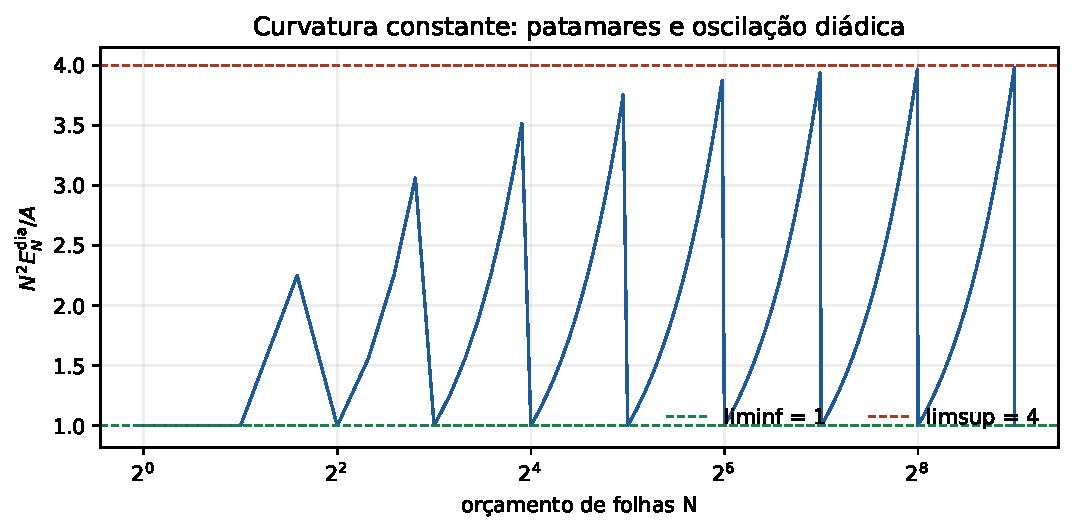
\includegraphics[width=.88\linewidth]{fig03_constante_quadratica.pdf}
 \caption{A normalização $N^2E_N^{\rm dia}/A$ reinicia em $1$ nas potências
 de dois e se aproxima de $4$ antes da potência seguinte.}
 \label{fig:quadratic-sawtooth}
\end{figure}

A \cref{tab:quadratic-exact} lista os valores racionais da lei, e a
\cref{fig:quadratic-sawtooth} exibe a oscilação normalizada entre as fases
diádicas consecutivas.

\subsection{Quadráticas por partes e lei de fase}

O caso seguinte separa a oscilação causada por uma única escala daquela
produzida por regiões com curvaturas diferentes.

\begin{theorem}[contagem exata em uma malha diádica base]
\label{thm:piecewise-quadratic-count}
Seja $\mathcal Q_{q_0}$ a partição uniforme de $K=[0,1]$ em células
$Q_i$ de comprimento $2^{-q_0}$. Suponha que $f\in C^1(K)$ seja quadrática
em cada $Q_i$ e
\[
 f''|_{\mathring Q_i}=\kappa_i\ne0,
 \qquad
 A_i=\frac{|\kappa_i||Q_i|^2}{8}.
\]
Existe $\varepsilon_0>0$ tal que, para
$0<\varepsilon<\varepsilon_0$,
\begin{equation}
 n_f(\varepsilon)
 =\sum_i2^{\lceil\log_4(A_i/\varepsilon)\rceil}.
 \label{eq:piecewise-count-law}
\end{equation}
Se $s=-\log_4\varepsilon$ e $a_i=\log_4A_i$, então
\begin{equation}
 \sqrt\varepsilon\,n_f(\varepsilon)
 =\Phi(s),
 \qquad
 \Phi(s)=\sum_i\sqrt{A_i}\,
 2^{\lceil s+a_i\rceil-(s+a_i)}.
 \label{eq:piecewise-phase-law}
\end{equation}
A função $\Phi$ é $1$-periódica e não constante. Portanto nem mesmo a
normalização em tolerância possui, em geral, um limite simples.
\end{theorem}

\begin{proof}
Todo ancestral da malha base que contém algum $Q_i$ é não afim, logo possui
erro local positivo. Como há apenas um número finito desses ancestrais,
escolha $\varepsilon_0$ menor que todos os seus erros e que todos os $A_i$.
O \cref{thm:threshold-optimality} obriga então a árvore de limiar a alcançar
cada $Q_i$. Dentro de $Q_i$, a identidade
\eqref{eq:quadratic-local-exact} mostra que são necessárias e suficientes
$2^{\lceil\log_4(A_i/\varepsilon)\rceil}$ folhas. Somar prova
\eqref{eq:piecewise-count-law}; a reescrita algébrica dá
\eqref{eq:piecewise-phase-law}. A periodicidade segue de
$\lceil s+1+a_i\rceil-(s+1+a_i)=\lceil s+a_i\rceil-(s+a_i)$.
Em qualquer intervalo aberto sem uma das finitíssimas fases de salto, todos
os tetos permanecem fixos e $\Phi$ é um múltiplo positivo de $2^{-s}$;
portanto é estritamente decrescente ali e não pode ser constante.
\end{proof}

\begin{corollary}[fases sincronizadas]
\label{cor:synchronized-phases}
Nas hipóteses do \cref{thm:piecewise-quadratic-count}, suponha ainda que
$A_i/A_j\in4^{\mathbb Z}$ para todos $i,j$. Então
\begin{equation}
 \liminf_{N\to\infty}N^2E_N^{\rm dia}(f)_\infty=\frac{I(f)^2}{8},
 \qquad
 \limsup_{N\to\infty}N^2E_N^{\rm dia}(f)_\infty=\frac{I(f)^2}{2}.
 \label{eq:synchronized-extremes}
\end{equation}
\end{corollary}

\begin{proof}
Escreva $A_i=A_\ast4^{-\rho_i}$ com $\rho_i\in\mathbb Z$ e, após deslocar
todos os índices, $\rho_i\ge0$. Para $r\ge\max_i\rho_i$, a tolerância
$\varepsilon_r=A_\ast4^{-r}$ produz
\[
 n_r=\sum_i2^{r-\rho_i}=C2^r,
 \qquad C=\sum_i2^{-\rho_i},
\]
folhas, todas com erro exatamente $\varepsilon_r$. Assim,
$E_{n_r}^{\rm dia}=\varepsilon_r$. Para reduzir o máximo estritamente, é
necessário subdividir cada uma das $n_r$ folhas; logo
$E_{2n_r-1}^{\rm dia}=\varepsilon_r$. Finalmente,
\[
 \sqrt{A_\ast}C=\sum_i\sqrt{A_i}=\frac{I(f)}{\sqrt8}.
\]
As duas sequências de orçamentos dão os extremos de
\eqref{eq:synchronized-extremes}; o envelope geral impede valores externos.
\end{proof}

A presença de sinais diferentes entre os $\kappa_i$ não altera essas
fórmulas: os erros locais dependem de $|\kappa_i|$. Para uma função global
$C^2$, uma mudança de sinal passa por zeros e a lei finita por fases deixa de
ser literalmente aplicável, mas o \cref{thm:general-dyadic-envelope} continua
válido sem alteração.

\begin{figure}[t]
 \centering
 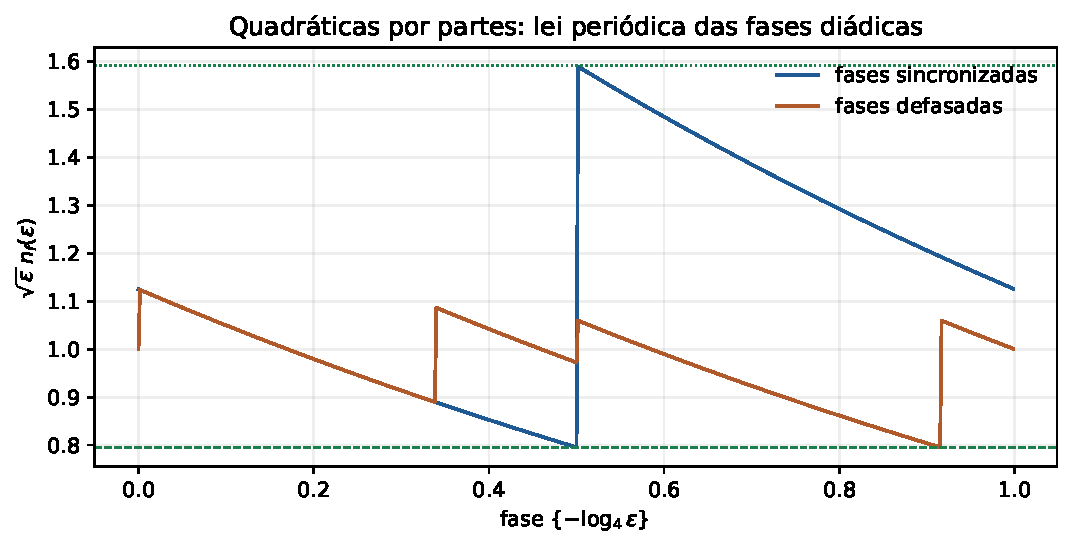
\includegraphics[width=.88\linewidth]{fig04_fases_piecewise.pdf}
 \caption{A lei \eqref{eq:piecewise-phase-law} em uma família sincronizada e
 outra defasada. Deslocar $-\log_4\varepsilon$ por uma unidade repete
 exatamente o perfil.}
 \label{fig:piecewise-phases}
\end{figure}

A sincronização e a defasagem previstas por
\eqref{eq:piecewise-phase-law} são comparadas na
\cref{fig:piecewise-phases}.

\subsection{Implementação e auditorias independentes}

O programa \texttt{constante\_diadica.py} implementa duas rotas que não
reutilizam a mesma recorrência: a árvore menos refinada do
\cref{thm:threshold-optimality} e uma programação dinâmica por número exato
de folhas,
\begin{equation}
 D(J,1)=e_f(J),\qquad
 D(J,n)=\min_{n_L+n_R=n}\max\{D(J_L,n_L),D(J_R,n_R)\}.
 \label{eq:independent-tree-dp}
\end{equation}
Para funções quadráticas por partes, $f$, $f'$, todos os pontos críticos e
todos os erros locais são calculados com \texttt{Fraction}. A fórmula
quadrática foi comparada com \eqref{eq:independent-tree-dp} para
$1\le N\le14$; a lei por partes foi confrontada com a construção explícita
do limiar em 14 escalas e a inversão do limiar foi comparada com a DP para
$1\le N\le12$.

Os dois diagnósticos $C^2$ usam apenas ponto flutuante determinístico para
avaliar extremos analíticos: $e^x$, cuja curvatura é estritamente positiva,
e $(x-1/2)^3$, cuja segunda derivada muda de sinal. Eles não participam de
nenhuma prova de igualdade; verificam apenas que os valores finitos
$\varepsilon n_f(\varepsilon)^2$ permanecem dentro do envelope teórico nas
$400$ tolerâncias examinadas.

\begin{remark}[agudeza uniforme e comportamento pontual]
\label{rem:envelope-not-pointwise}
O \cref{thm:general-dyadic-envelope} é agudo \emph{uniformemente sobre a
classe} $C^2$: a mesma função quadrática do
\cref{thm:quadratic-dyadic-constant} realiza $I(f)^2/8$ e $I(f)^2/2$ ao longo
de subsequências. Logo as duas constantes são ótimas em teoremas uniformes
sobre $C^2$. Para uma função fixa, o conjunto de acumulação pode ser um
subconjunto próprio do envelope.

No modelo finito do \cref{thm:piecewise-quadratic-count}, essa distinção pode
ser tornada exata. Ponha $w_i=\sqrt{A_i}$ e considere os resíduos de
$a_i=\log_4A_i$ módulo $1$. Cada fator
\[
 g(s+a_i)=2^{\lceil s+a_i\rceil-(s+a_i)}
\]
pertence a $[1,2)$ e vale $1$ precisamente quando $s+a_i\in\mathbb Z$. Se os
resíduos não são todos iguais, não existe fase que torne simultaneamente
todos os fatores iguais a $1$, nem uma sequência de fases que os faça tender
simultaneamente a $2$. Como há apenas um número finito de fases de salto no
círculo, existem $\delta_-,\delta_+>0$ tais que
\[
 \frac{I(f)}{\sqrt8}+\delta_-
 \le \Phi(s)
 \le \frac{I(f)}{\sqrt2}-\delta_+
 \qquad(s\in\mathbb R).
\]
Assim, a normalização dual $\varepsilon n_f(\varepsilon)^2$ permanece
estritamente dentro do envelope para todas as tolerâncias suficientemente
pequenas nessa família defasada. No caso sincronizado, a condição
$A_i/A_j\in4^{\mathbb Z}$ do \cref{cor:synchronized-phases} alinha os
resíduos e permite recuperar os extremos.

A prova finita usa o número discreto de fases de salto e, portanto, é
específica da curvatura quadrática por partes. A
\cref{tab:smooth-diagnostics} registra que, em $400$ tolerâncias entre
$10^{-3}$ e $10^{-10}$, os dois exemplos suaves permanecem estritamente no
interior. A caracterização, para $f$ dada, do conjunto exato de acumulação de
$N^2E_N^{\rm dia}(f)_\infty$ dentro de
$[I(f)^2/8,I(f)^2/2]$ constitui o problema de fases para curvatura variável.
\end{remark}

\begin{table}[t]
 \centering
 \caption{Diagnósticos determinísticos em 400 tolerâncias entre
 $10^{-3}$ e $10^{-10}$. As colunas externas são teóricas.}
 \label{tab:smooth-diagnostics}
 \small
 \begin{tabular}{lrrr}
\toprule
função & $I(f)^2/8$ & faixa observada de $\varepsilon n_f(\varepsilon)^2$ & $I(f)^2/2$ \\
\midrule
$e^x$ & 0.210420 & [0.339008, 0.515293] & 0.841679 \\
$(x-\frac{1}{2})^3$ & 0.166667 & [0.275877, 0.417099] & 0.666667 \\
\bottomrule
\end{tabular}

\end{table}

\begin{figure}[t]
 \centering
 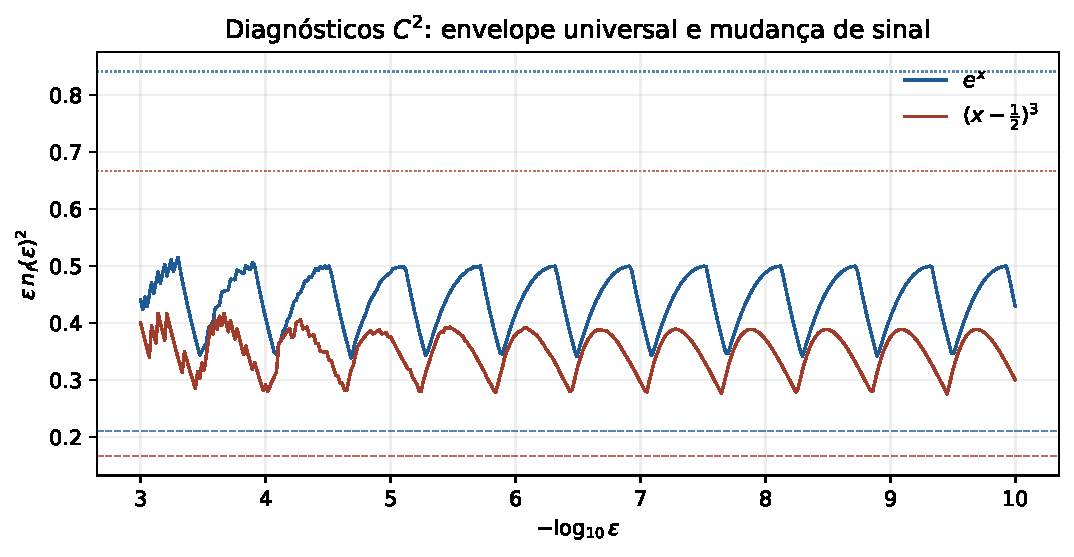
\includegraphics[width=.88\linewidth]{fig05_envelope_c2.pdf}
 \caption{Diagnósticos para curvatura positiva e para mudança de sinal. As
 linhas tracejadas e pontilhadas são, respectivamente, $I(f)^2/8$ e
 $I(f)^2/2$.}
 \label{fig:c2-envelope}
\end{figure}

Os dois exemplos suaves da \cref{fig:c2-envelope} permanecem dentro do
envelope teórico em todas as tolerâncias auditadas.

\begin{table}[t]
 \centering
 \caption{Auditoria executável das constantes diádicas.}
 \label{tab:dyadic-constants-audit}
 \small
 \begin{tabularx}{\linewidth}{@{}Xr@{}}
\toprule
Verificação & resultado \\
\midrule
Fórmula quadrática $=$ DP independente & true \\
Limiar quadrático $=$ contagem fechada & true \\
Contagem por partes $=$ árvore de limiar & true \\
DP por partes $=$ inversão do limiar & true \\
Fases sincronizadas atingem os dois extremos & true \\
Diagnóstico $C^2$ positivo dentro do envelope & true \\
Mudança de sinal dentro do envelope & true \\
Varreduras suaves estritamente interiores (400 pontos) & true \\
Execução sem números pseudoaleatórios & true \\
\bottomrule
\end{tabularx}

\end{table}

A \cref{tab:dyadic-constants-audit} reúne, em uma única trilha, as
identidades exatas e os testes independentes desta seção.

\subsection{Compatibilidade com a altura aritmética}

Os teoremas desta seção permitem todos os descendentes da raiz. Na biblioteca
$\Library$, uma malha uniforme de profundidade relativa $r$ em
$K=J_{k_0,m_0}$, $m_0\ge0$, só está espacialmente disponível quando
\[
 H\ge k_0+r+1,
 \qquad H\ge2^r(m_0+1)
\]
pela \cref{prop:translation-obstruction}. Como as escalas relevantes têm
$2^r\asymp N$, a segunda condição já força $H=\Omega(N(m_0+1))$, antes de
se contabilizar a altura necessária para racionalizar os valores nodais.
Assim, a passagem de \eqref{eq:budget-envelope} para uma agenda $H(N)$ inclui
esse acoplamento geométrico.

Para cada árvore fixa, o teorema de racionalização da \cref{sec:assemblies}
aproxima os valores nodais reais por racionais compartilhados e aproxima
$P_\Lambda f$ arbitrariamente bem por uma montagem da biblioteca. Os
interpolantes pertencem, portanto, à aderência quando a altura cresce. O
problema interpolatório \eqref{eq:optimal-dyadic-interpolation} e o melhor
erro racional com deslocamentos nodais são objetos distintos; a constante
assintótica do segundo sob uma agenda fixa de altura permanece em aberto.

\section{Classes de aproximação sob uma agenda de altura}
\label{sec:approximation-classes}

O número de folhas e a altura aritmética desempenham papéis independentes. A
racionalização por denominador comum absorve o fator da malha e fornece
altura suficiente $N^2$ no caso $s=2$. Ao mesmo tempo, catálogos racionais de
altura fixa falham em ser invariantes por escalares reais. O funcional
associado será, por isso, formulado como funcional de taxa e sua obstrução de
homogeneidade será demonstrada explicitamente.

\subsection{Erro apontado e funcional de taxa}

Seja $H:\mathbb N\to\mathbb N$, $H(N)\ge2$, uma agenda não decrescente.
Estenda a notação $\Aclass_{N,H}(K)$ ao caso $N=1$ pela mesma
definição: no máximo uma folha e altura no máximo $H$. Essa classe pode não
conter a função nula, pois a
biblioteca exclui inclinações nulas. Para obter um erro com ponto-base sem
alterar nenhum aproximante não nulo, ponha
\begin{equation}
 \Sigma_N^{\Library,H}(K)
 :=\{0\}\cup\Aclass_{N,H(N)}(K),
 \qquad
 e_N^{\Library,H}(f)
 :=\inf_{g\in\Sigma_N^{\Library,H}(K)}\|f-g\|_{\infty,K}.
 \label{eq:pointed-error}
\end{equation}
Em termos do erro conjunto da \cref{sec:complexity}, estendido pela mesma fórmula
ao caso $N=1$,
\begin{equation}
 e_N^{\Library,H}(f)
 =\min\bigl\{\|f\|_{\infty,K},
 E_{N,H(N)}^{\Library}(f)_\infty\bigr\}.
 \label{eq:pointed-inherited}
\end{equation}
A origem completa o esquema apontado usado para medir taxas.

\begin{proposition}[aninhamento da agenda]
\label{prop:schedule-nesting}
Se $H$ é não decrescente, então
\begin{equation}
 \Sigma_N^{\Library,H}(K)
 \subseteq\Sigma_{N+1}^{\Library,H}(K)
 \quad\text{e}\quad
 e_{N+1}^{\Library,H}(f)\le e_N^{\Library,H}(f)\le\|f\|_\infty.
 \label{eq:schedule-nesting}
\end{equation}
Para cada $N$, o ínfimo em \eqref{eq:pointed-error} é atingido.
\end{proposition}

\begin{proof}
Uma representação com no máximo $N$ folhas e altura no máximo $H(N)$
continua admissível sob os limites $N+1$ e $H(N+1)$. A função nula pertence
a ambas as classes. Isso prova as inclusões e as desigualdades. O calibre de
altura limita escala, translação, valor central e inclinação; portanto há
somente um número finito de átomos e de árvores admissíveis. Assim
$\Sigma_N^{\Library,H}(K)$ é finito e a distância mínima é atingida.
\end{proof}

A definição de classes por sequências de melhores erros é padrão na teoria de
espaços de aproximação não linear \citep{devore1998}. O funcional seguinte
acrescenta a essa construção o catálogo apontado e a agenda aritmética de
altura.

Para $\alpha>0$ e $0<q\le\infty$, defina o \emph{funcional de taxa}
\begin{align}
 \mathfrak a_{\alpha,q}^{\Library,H}(f)
 &:=\left(\sum_{N=1}^{\infty}
       \bigl[N^\alpha e_N^{\Library,H}(f)\bigr]^q\frac1N
       \right)^{1/q}, &&0<q<\infty,
 \label{eq:rate-functional-finite}\\
 \mathfrak a_{\alpha,\infty}^{\Library,H}(f)
 &:=\sup_{N\ge1}N^\alpha e_N^{\Library,H}(f).
 \label{eq:rate-functional-infty}
\end{align}
Escreva
\begin{equation}
 \mathscr A_{q}^{\alpha}(\Library,H)
 :=\{f\in C(K):\mathfrak a_{\alpha,q}^{\Library,H}(f)<\infty\}.
 \label{eq:approximation-stratum}
\end{equation}
O termo \emph{classe} ou \emph{estrato} será usado para
\eqref{eq:approximation-stratum}; \emph{espaço quase-normado} será reservado
a situações em que homogeneidade e quase-triângulo tenham sido efetivamente
provados. Essa distinção é necessária no catálogo presente e não ocorre
automaticamente a partir da literatura de esquemas cônicos ou de redes
\citep{gribonval2022,grohs2023}.

\begin{theorem}[redução exata às escalas diádicas]
\label{thm:dyadic-rate-equivalence}
Para toda agenda não decrescente, $\alpha>0$ e $0<q\le\infty$,
\begin{equation}
 \mathfrak a_{\alpha,q}^{\Library,H}(f)
 \asymp_{\alpha,q}
 \left\|\bigl(2^{r\alpha}
 e_{2^r}^{\Library,H}(f)\bigr)_{r\ge0}\right\|_{\ell^q},
 \label{eq:dyadic-rate-equivalence}
\end{equation}
com a interpretação usual por supremo quando $q=\infty$. As constantes não
dependem de $f$ nem de $H$.
\end{theorem}

\begin{proof}
No bloco $2^r\le N<2^{r+1}$, a monotonicidade fornece
\[
 e_{2^{r+1}}^{\Library,H}(f)
 \le e_N^{\Library,H}(f)
 \le e_{2^r}^{\Library,H}(f),
\]
enquanto $2^{r\alpha}\le N^\alpha<2^{(r+1)\alpha}$ e
\[
 \sum_{N=2^r}^{2^{r+1}-1}\frac1N\asymp1.
\]
Somar as duas estimativas de bloco e deslocar o índice inferior por uma
unidade prova \eqref{eq:dyadic-rate-equivalence}. Para $q=\infty$, basta
tomar o supremo nos mesmos blocos.
\end{proof}

\subsection{Por que o funcional bruto não é uma quase-norma}

\begin{proposition}[falha exata de homogeneidade]
\label{prop:nonhomogeneous-functional}
Suponha $K=[0,1]$ e $H(1)\ge2$. O funcional
$\|f\|_\infty+\mathfrak a_{\alpha,q}^{\Library,H}(f)$ não é homogêneo sobre
$C(K)$ e, portanto, não é uma quase-norma. Mais precisamente, para
$f(x)=x$ e $c=\sqrt2$,
\begin{equation}
 \mathfrak a_{\alpha,q}^{\Library,H}(f)=0,
 \qquad
 \mathfrak a_{\alpha,q}^{\Library,H}(cf)>0.
 \label{eq:nonhomogeneous-certificate}
\end{equation}
\end{proposition}

\begin{proof}
A função $f(x)=x$ é o átomo $(k,m,y_0,s)=(0,0,1/2,1)$, de altura $2$.
Logo $f\in\Sigma_N^{\Library,H}(K)$ para todo $N$ e todos os erros de
$f$ são nulos. Por outro lado, toda função não nula em
$\Sigma_1^{\Library,H}(K)$ possui inclinação racional em $[0,1]$, enquanto
$cf$ possui inclinação irracional $\sqrt2$. Como o primeiro catálogo é
finito, $cf$ tem distância estritamente positiva a ele. Assim o termo
$N=1$ de \eqref{eq:rate-functional-finite}, ou o mesmo termo no supremo,
é positivo. Consequentemente,
\[
 \|cf\|_\infty+\mathfrak a_{\alpha,q}^{\Library,H}(cf)
 >|c|\bigl(\|f\|_\infty+
 \mathfrak a_{\alpha,q}^{\Library,H}(f)\bigr).
\]
\end{proof}

\begin{remark}[estrutura aritmética do funcional]
\label{rem:quasinorm-scope}
Adicionar $0$ fornece o ponto-base, enquanto a obstrução de homogeneidade real
permanece. O fecho cônico ou o envoltório linear admite escalares reais
externos e elimina o custo aritmético medido por $H$. Assim, os objetos
naturais são os estratos \eqref{eq:approximation-stratum} e seus funcionais de
taxa.
\end{remark}

\section{Teoremas diretos e agendas de altura}
\label{sec:direct-height}

O paradigma de teoremas diretos e inversos tem antecedentes tanto na
aproximação por splines e em espaços de Besov quanto na aproximação por funções
racionais \citep{petrushev1988,petrushevpopov1987}. Nesta última expressão,
``racional'' significa quociente de polinômios, e não a aritmética dos
coeficientes da biblioteca; o elemento novo desta seção é acompanhar
explicitamente a altura desses coeficientes.

Fixe a raiz diádica $K=J_{k_0,m_0}$ e escreva $L=|K|=2^{-k_0}$. Para
$f\in C(K)$, defina
\begin{align}
 \omega_1(f,t)_{\infty,K}
 &=\sup_{\substack{0<h\le t\\x,x+h\in K}}
   |f(x+h)-f(x)|,\label{eq:first-modulus}\\
 \omega_2(f,t)_{\infty,K}
 &=\sup_{\substack{0<h\le t\\x,x+2h\in K}}
   |f(x+2h)-2f(x+h)+f(x)|.
 \label{eq:second-modulus-direct}
\end{align}
Para $0<s<2$ e $0<q\le\infty$, usaremos a caracterização diádica equivalente da
quase-norma de Besov
\begin{equation}
 \|f\|_{B^s_{\infty,q}(K)}^*
 :=\|f\|_{\infty,K}
 +\left\|\bigl(2^{rs}\omega_2(f,L2^{-r})_{\infty,K}
           \bigr)_{r\ge0}\right\|_{\ell^q}.
 \label{eq:dyadic-besov-norm}
\end{equation}
Ela é equivalente à definição integral com medida $\dd t/t$; essa
discretização é clássica e decorre das desigualdades de escala do módulo de
suavidade \citep{devorelorentz1993,devorepopov1988}.

Também será usada a desigualdade de Whitney de ordem dois
\citep{whitney1957,devore1998}: existe uma
constante universal $C_W$ tal que, em todo subintervalo $J\subset K$,
\begin{equation}
 \inf_{\ell\ \text{afim}}\|f-\ell\|_{\infty,J}
 \le C_W\omega_2(f,|J|)_{\infty,J}.
 \label{eq:whitney-direct}
\end{equation}
Como o interpolador nos extremos reproduz funções afins e tem norma de
operador $1$, seu erro é no máximo duas vezes o lado direito.

Ponha
\begin{equation}
 \nu_s=\max\{1,s\},
 \qquad C_K=4(k_0+|m_0|+2).
 \label{eq:height-schedule-constants}
\end{equation}

\subsection{Racionalização com denominador comensurável}

A prova precisa acompanhar também primeiras diferenças. A desigualdade de
Marchaud de ordens um e dois
\citep{devorelorentz1993,lorentz1996} implica, para $0<t\le L/2$,
\begin{equation}
 \omega_1(f,t)_{\infty,K}
 \le C_s\|f\|_{B^s_{\infty,\infty}(K)}^*
 \begin{cases}
  (t/L)^s,&0<s<1,\\
  (t/L)\log(eL/t),&s=1,\\
  t/L,&1<s<2.
 \end{cases}
 \label{eq:marchaud-regimes}
\end{equation}
Essa é exatamente a informação necessária para limitar a inclinação quando
o denominador disponível é menor que o inverso da malha.

\begin{lemma}[Jackson racional com altura explícita]
\label{lem:rational-jackson-height}
Seja $f\in B^s_{\infty,\infty}(K)$, $R=\|f\|_\infty$. Existe
$n_0=n_0(f,K,s)$ tal que, para toda potência de dois $n=2^r\ge n_0$ e todo
inteiro
\[
 H\ge\max\{C_Kn^{\nu_s},16(R+1)\}
\]
que satisfaça
\begin{equation}
 H\ge\max\{2,k_0+r+1,
      \max_{0\le j<n}|2^rm_0+j|+1\},
 \label{eq:height-geometry-condition}
\end{equation}
existe $g_{n,H}\in\Aclass_{n,H}(K)$ tal que
\begin{equation}
 \|f-g_{n,H}\|_\infty
 \le 2C_W\omega_2(f,L/n)_{\infty,K}
      +\frac{C(R+1)}{H},
 \label{eq:rational-jackson-height}
\end{equation}
onde $C$ é absoluto e $C_W$ é a constante de Whitney.

Além disso, existe $A_{K,s}\ge1$, independente de $f$, com a seguinte versão
uniforme. Se $B\ge1$, $\|f\|_{B^s_{\infty,\infty}(K)}^*\le B$, $n=2^r\ge2$
e
\begin{equation}
 H\ge A_{K,s}(B+1)n^{\nu_s},
 \label{eq:uniform-ball-height-threshold}
\end{equation}
então todas as conclusões anteriores valem sem limiar dependente de $f$ e com
o último termo de \eqref{eq:rational-jackson-height} igual a
$8(B+1)/H$. A constante $A_{K,s}$ também torna automática a condição
geométrica \eqref{eq:height-geometry-condition}.
\end{lemma}

\begin{proof}
Escolha a maior potência de dois $Q$ tal que
$8(R+1)Q\le H$. Para $H\ge16(R+1)$,
\begin{equation}
 \frac{H}{16(R+1)}<Q\le\frac{H}{8(R+1)}.
 \label{eq:Q-window}
\end{equation}
Nos nós $t_j=\inf K+jL/n$, use as grades alternadas
\[
 G_j=\frac1Q\left(\mathbb Z+\frac{j\bmod2}{2}\right)
\]
e escolha $v_j\in G_j$ mais próximo de $f(t_j)$; se os dois vizinhos da grade
forem equidistantes, escolha o menor. Então
$|v_j-f(t_j)|\le(2Q)^{-1}$ e $v_j\ne v_{j+1}$. Escrevendo
$v_j=b_j/(2Q)$ com $b_j\equiv j\pmod2$, obtém-se
\begin{equation}
 |b_j|\le2QR+1.
 \label{eq:general-b-bound}
\end{equation}
Na célula $J_{k_0+r,2^rm_0+j}$, os parâmetros são
\begin{equation}
 y_{0,j}=\frac{b_j+b_{j+1}}{4Q},
 \qquad
 s_j=2^{k_0+r}\frac{b_{j+1}-b_j}{2Q}.
 \label{eq:general-atom-parameters}
\end{equation}
A janela \eqref{eq:Q-window} e \eqref{eq:general-b-bound} dão
$\height(y_{0,j})\le H$. Como $b_{j+1}-b_j$ é ímpar, não há cancelamento
oculto com $2Q$. Se $2^{k_0+r}\le2Q$, a fração reduzida de $s_j$ tem
numerador $b_{j+1}-b_j$ e denominador $2Q/2^{k_0+r}$; a cota grosseira
$|b_{j+1}-b_j|\le4QR+2$ prova $\height(s_j)\le H$ após um aumento absoluto
do limiar inicial.

Se $2^{k_0+r}>2Q$, a inclinação é inteira e
\begin{equation}
 |s_j|
 \le \frac nL\left(\omega_1(f,L/n)+\frac1Q\right).
 \label{eq:slope-marchaud-bound}
\end{equation}
Nos três regimes de \eqref{eq:marchaud-regimes}, o primeiro termo é limitado,
respectivamente, por
\[
 C_{K,s}\|f\|_{B^s_{\infty,\infty}}^*n^{1-s},\qquad
 C_{K}\|f\|_{B^1_{\infty,\infty}}^*\log(en),\qquad
 C_{K,s}\|f\|_{B^s_{\infty,\infty}}^*;
\]
o segundo é $O((R+1)n/H)$. Com o coeficiente fixo da primeira parte, essas
quantidades ficam abaixo de $H$ quando $n\ge n_0(f,K,s)$. Se a norma é no
máximo $B$, as desigualdades elementares
$n^{1-s}\le n$, $\log(en)\le2n$ e $1\le n^{\nu_s}$, juntamente com
\eqref{eq:uniform-ball-height-threshold}, dão a mesma conclusão para todo
$n\ge2$ após escolher $A_{K,s}$ suficientemente grande. Como
\[
 k_0+r+1\le C_Kn,\qquad
 \max_{0\le j<n}|2^rm_0+j|+1\le(|m_0|+1)n+1,
\]
essa escolha também cobre a geometria. Logo cada peça pertence a
$\Library_H$ em ambas as versões.

Se $P_nf$ é o interpolante dos valores exatos nos mesmos nós, a estimativa
de Whitney \eqref{eq:whitney-direct} dá
\[
 \|f-P_nf\|_\infty
 \le2C_W\omega_2(f,L/n)_{\infty,K}.
\]
A diferença entre os dois interpolantes é, em cada célula, uma combinação
convexa dos erros nodais e não excede $(2Q)^{-1}$. Usando
\eqref{eq:Q-window}, esse termo é estritamente menor que
$8(R+1)/H\le8(B+1)/H$ na versão uniforme. Isso prova as duas afirmações.
\end{proof}

\subsection{Imersão direta sem o expoente espúrio}

Para $\kappa\ge0$, defina a agenda inteira
\begin{equation}
 H_{s,\kappa}(N)
 =\left\lceil C_K(N+1)^{\nu_s}
        [\log(eN)]^\kappa\right\rceil.
 \label{eq:corrected-height-schedule}
\end{equation}
Ela é não decrescente e satisfaz a obstrução geométrica de
\eqref{eq:height-geometry-condition} em toda malha uniforme com no máximo
$N$ folhas.

\begin{theorem}[direção direta com altura aritmética]
\label{thm:direct-besov-height}
Se $0<s<2$, então as seguintes inclusões de conjuntos valem:
\begin{align}
 B^s_{\infty,\infty}(K)
 &\subset
 \mathscr A^s_\infty(\Library,H_{s,0}),
 \label{eq:direct-endpoint}\\
 B^s_{\infty,q}(K)
 &\subset
 \mathscr A^s_q(\Library,H_{s,0}),
 &&0<q<\infty,\qquad 0<s<1,
 \label{eq:direct-subcritical}\\
 B^s_{\infty,q}(K)
 &\subset
 \mathscr A^s_q(\Library,H_{s,\kappa}),
 &&0<q<\infty,\qquad 1\le s<2,\qquad\kappa>1/q.
 \label{eq:direct-critical-log}
\end{align}
Em particular, para $s\ge1$, o endpoint $q=\infty$ admite
$H(N)=O_K(N^s)$; para $q<\infty$, basta acrescentar um fator logarítmico
crítico. Como
alternativa sem logaritmo, para qualquer $\eta>0$ pode-se substituir
$H_{s,\kappa}$ em \eqref{eq:direct-critical-log} por
\begin{equation}
 \widetilde H_{s,\eta}(N)
 =\left\lceil C_K(N+1)^{\max\{1,s+\eta\}}\right\rceil.
 \label{eq:polynomial-slack-schedule}
\end{equation}
\end{theorem}

\begin{proof}
Seja $n=2^r$. Para $r$ suficientemente grande, o
\cref{lem:rational-jackson-height} aplicado a
$H=H_{s,\kappa}(n)$ dá
\begin{equation}
 n^s e_n^{\Library,H}(f)
 \le C n^s\omega_2(f,L/n)_{\infty,K}
     +C_f\frac{n^s}{H_{s,\kappa}(n)}.
 \label{eq:direct-sequence-bound}
\end{equation}
Um número finito de escalas iniciais não afeta pertinência a $\ell^q$. O
primeiro termo do lado direito pertence a $\ell^q$ por
\eqref{eq:dyadic-besov-norm}. Se $s<1$, o segundo decai geometricamente como
$n^{s-1}$. Se $s\ge1$, ele é $O(r^{-\kappa})$, pois
$\log(en)\asymp r$; pertence a $\ell^q$ quando $\kappa q>1$ e é limitado
quando $q=\infty$ e $\kappa=0$. A agenda
\eqref{eq:polynomial-slack-schedule} produz, em vez disso, o fator
$n^{-\eta}$. O \cref{thm:dyadic-rate-equivalence} transfere as conclusões
das potências de dois para todos os orçamentos $N$.
\end{proof}

O limiar $n_0(f,K,s)$ do primeiro enunciado não impede uniformidade sobre
conjuntos normados: a segunda parte do
\cref{lem:rational-jackson-height} permite calibrar uma única agenda para uma
bola inteira. A formulação quantitativa seguinte é deliberadamente em termos
de bolas, porque o funcional de taxa não é homogêneo sobre escalares reais
pela \cref{prop:nonhomogeneous-functional}.

\begin{corollary}[imersões quantitativas uniformes sobre bolas]
\label{cor:uniform-besov-ball-embedding}
Para $B\ge1$ e $\kappa\ge0$, defina
\begin{equation}
 \widehat H_{s,\kappa}^{[B]}(N)
 =\left\lceil A_{K,s}(B+1)(N+1)^{\nu_s}
        [\log(eN)]^\kappa\right\rceil .
 \label{eq:ball-calibrated-height-schedule}
\end{equation}
Existem constantes independentes de $B$ e de $f$ tais que
\begin{align}
 \sup_{\|f\|_{B^s_{\infty,\infty}(K)}^*\le B}
 \mathfrak a_{s,\infty}^{\Library,
       \widehat H_{s,0}^{[B]}}(f)
 &\le C_{K,s}(B+1), &&0<s<2,\label{eq:uniform-ball-endpoint}\\
 \sup_{\|f\|_{B^s_{\infty,q}(K)}^*\le B}
 \mathfrak a_{s,q}^{\Library,
       \widehat H_{s,0}^{[B]}}(f)
 &\le C_{K,s,q}(B+1), &&0<s<1,\quad0<q<\infty,
 \label{eq:uniform-ball-subcritical}\\
 \sup_{\|f\|_{B^s_{\infty,q}(K)}^*\le B}
 \mathfrak a_{s,q}^{\Library,
       \widehat H_{s,\kappa}^{[B]}}(f)
 &\le C_{K,s,q,\kappa}(B+1),
 &&1\le s<2,\quad0<q<\infty,\quad\kappa>1/q.
 \label{eq:uniform-ball-critical}
\end{align}
Assim, cada bola de Besov é enviada uniformemente a uma bola do funcional de
taxa sob uma única agenda, sem qualquer limiar dependente da função.
\end{corollary}

\begin{proof}
Para $n=2^r\ge2$, a versão uniforme do
\cref{lem:rational-jackson-height} fornece
\[
 n^s e_n^{\Library,\widehat H}(f)
 \le C_{K,s}n^s\omega_2(f,L/n)_{\infty,K}
 +C_{K,s}\frac{n^s}{n^{\nu_s}[\log(en)]^\kappa}.
\]
O primeiro termo tem norma $\ell^q$ limitada por $C_{K,s}B$ na
caracterização \eqref{eq:dyadic-besov-norm}. O segundo é limitado para
$q=\infty$; é geometricamente somável se $s<1$ e $\kappa=0$; e pertence a
$\ell^q$ se $s\ge1$ e $\kappa q>1$. A escala $N=1$ é limitada por
$\|f\|_\infty\le B$. A equivalência diádica do
\cref{thm:dyadic-rate-equivalence} conclui as três cotas.
\end{proof}

\begin{remark}[o papel do índice $q$]
\label{rem:q-height-role}
O denominador comum determina o expoente aritmético e o índice $q$ determina
a somabilidade. Uma quantização de ordem
$H(N)^{-1}=N^{-s}$ deixa o termo normalizado $N^se_N$ apenas limitado; isso
é suficiente para o supremo, mas a sequência constante não pertence a
$\ell^q$ para $q<\infty$. O fator $[\log(eN)]^\kappa$, $\kappa>1/q$, torna
\[
 \sum_{N\ge2}\frac1{N[\log(eN)]^{\kappa q}}<\infty.
\]
Esse fator logarítmico é suficiente no argumento uniforme por
racionalização.
\end{remark}

\subsection{Endpoint quadrático e agudeza da agenda construtiva}

\begin{corollary}[endpoint $C^2$]
\label{cor:c2-direct-endpoint}
Na raiz $K=[0,1]$, seja
$\mathcal F_{R,M}=\{f\in C^2[0,1]:\|f\|_\infty\le R,
\|f''\|_\infty\le M\}$ e
\[
 C_H=\max\{4(R+1),\,2(4R+M/2+1)\}.
\]
Com $H_2(N)=\lceil C_HN^2\rceil$,
\begin{equation}
 \sup_{f\in\mathcal F_{R,M}}
 \mathfrak a_{2,\infty}^{\Library,H_2}(f)
 \le\max\left\{R,\frac{M+4}{2}\right\}.
 \label{eq:c2-direct-endpoint}
\end{equation}
As montagens que realizam a cota para $N\ge2$ usam
$O_{R,M}(N\log(2N))$ bits nos três formatos prefix-free do
\cref{thm:coding-formats}.
\end{corollary}

\begin{proof}
A \cref{thm:joint-budget} fornece, para todo $N\ge2$,
\[
 E_{N,\lceil C_HN^2\rceil}^{\Library}(f)_\infty
 <\frac{M+4}{2N^2}.
\]
O erro apontado não é maior que esse erro; para $N=1$, ele não excede
$\|f\|_\infty\le R$. Tomar o supremo prova
\eqref{eq:c2-direct-endpoint}. A afirmação de bits é a mesma construção,
sem alteração de formato.
\end{proof}

Há um sentido uniforme no qual o expoente aritmético $s$ não pode ser
reduzido por esse tipo de teorema. Denote
$\mathcal Q_H=\{p/q\in\mathbb Q:\height(p/q)\le H\}$.

\begin{proposition}[piso aritmético uniforme]
\label{prop:arithmetic-floor}
Para cada $H\ge2$, seja $a_H=1/(2H)$ e $f_H\equiv a_H$ em $K$. Então, para
todo $N$,
\begin{equation}
 e_N^{\Library,H}(f_H)
 \ge\operatorname{dist}(a_H,\mathcal Q_H)
 =\frac1{2H}.
 \label{eq:arithmetic-floor}
\end{equation}
Consequentemente, se uma classe contém todas as constantes
$f\equiv a$, $|a|\le1/4$, e satisfaz
$\sup_f e_N^{\Library,H}(f)\le C N^{-s}$, então
$H(N)\ge(2C)^{-1}N^s$ para todo $N$ com $H(N)\ge2$.
\end{proposition}

\begin{proof}
No centro de qualquer folha, uma montagem não nula assume o valor central
$y_0\in\mathcal Q_H$ do átomo; a função nula assume o valor $0$, que também
pertence a $\mathcal Q_H$. Não existe racional de altura no máximo $H$
estritamente entre $0$ e $1/H$: todo racional positivo nessa faixa teria
numerador pelo menos $1$ e denominador maior que $H$. Portanto
$a_H$ está a distância $1/(2H)$ de $\mathcal Q_H$. Avaliar o erro em um
centro de folha prova a cota. Como $a_{H(N)}\le1/4$, a hipótese uniforme
aplicada a essa constante dá
$1/(2H(N))\le CN^{-s}$, que é a última afirmação.
\end{proof}

Por outro lado, a \cref{prop:translation-obstruction} mostra que a malha
uniforme de $N=2^r$ folhas em $[0,1]$ só está inteiramente disponível quando
$H\ge N$. Assim, a construção uniforme combina dois pisos distintos:
\begin{equation}
 H(N)\gtrsim N^s\quad\text{(aritmética)},
 \qquad
 H(N)\gtrsim N\quad\text{(geometria uniforme)}.
 \label{eq:two-height-floors}
\end{equation}
Isso explica o expoente $\max\{1,s\}$ em
\eqref{eq:corrected-height-schedule}. A segunda cota é a barreira geométrica
da realização por malha uniforme sob o calibre atual; métodos adaptativos
possuem distribuições de folhas distintas.

\subsection{Validação executável}

A \cref{tab:height-schedules} resume as agendas provadas.
\begin{table}[t]
 \centering
 \small
 \begin{tabularx}{\linewidth}{@{}cclX@{}}
\toprule
regularidade & $q$ & agenda suficiente & mecanismo dominante\\
\midrule
$0<s<1$ & $0<q\le\infty$ & $H(N)\asymp N$ & geometria; a quantização $H^{-1}$ é subcrítica\\
$1\le s<2$ & $q=\infty$ & $H(N)\asymp N^s$ & altura da ordenada racional\\
$1\le s<2$ & $q<\infty$ & $H(N)\asymp N^s\log^\kappa(eN)$, $\kappa>1/q$ & somabilidade do piso aritmético\\
$1\le s<2$ & $q<\infty$ & $H(N)\asymp N^{s+\eta}$, $\eta>0$ & alternativa puramente polinomial\\
$s=2$ & $q=\infty$ & $H(N)\asymp N^2$ & endpoint uniforme de $C^2$\\
\bottomrule
\end{tabularx}

 \caption{Agendas suficientes. O fator logarítmico pertence à
 somabilidade para $q<\infty$, não à propagação algébrica da inclinação.}
 \label{tab:height-schedules}
\end{table}

O caso $f_\star(x)=4x(x-1)$ realiza exatamente a construção do
\cref{thm:joint-budget}.
Na \cref{tab:height-audit}, $\height(y_0)$ e $\height(s)$ são os
máximos efetivos entre as folhas; $4N^2$ é a escala efetiva observada e
$N^3$ é exibido apenas como escala comparativa.
\begin{table}[t]
 \centering
 \small
 \begin{tabular}{rrrrrr}
\toprule
$N$ & $\height(y_0)$ & $\height(s)$ & $H_{\rm efetivo}$ & $4N^2$ & $N^3$\\
\midrule
4 & 64 & 25 & 64 & 64 & 64\\
8 & 256 & 57 & 256 & 256 & 512\\
16 & 1024 & 121 & 1024 & 1024 & 4096\\
32 & 4096 & 249 & 4096 & 4096 & 32768\\
64 & 16384 & 505 & 16384 & 16384 & 262144\\
128 & 65536 & 1017 & 65536 & 65536 & 2097152\\
\bottomrule
\end{tabular}

 \caption{Auditoria racional exata da agenda para $f_\star$. Em $N=32$ e
 $128$, recuperam-se respectivamente
 $(\height(y_0),\height(s))=(4096,249)$ e $(65536,1017)$. Os valores
 tabulados são exatos; em
 \texttt{resultados\_espacos\_aproximacao.json}, somente os diagnósticos
 logarítmicos auxiliares são armazenados em ponto flutuante e, por isso, não
 se exige identidade byte a byte desses campos entre plataformas.}
 \label{tab:height-audit}
\end{table}

\begin{figure}[t]
 \centering
 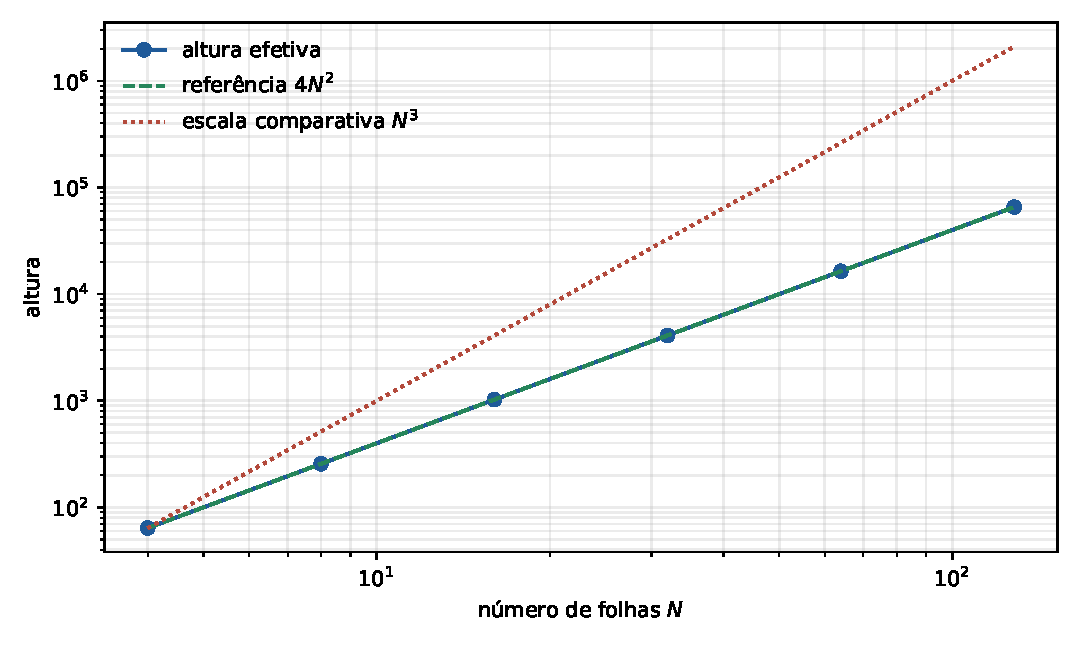
\includegraphics[width=.88\linewidth]{fig_altura_agendas.pdf}
 \caption{A altura efetiva da construção quadrática acompanha $N^2$; a
 curva $N^3$ corresponde ao fator de malha que o denominador comum absorve.}
 \label{fig:height-schedules}
\end{figure}

A \cref{fig:height-schedules} confirma, na construção quadrática auditada, a
separação entre a agenda provada $N^2$ e a escala comparativa $N^3$.

O programa \texttt{espacos\_aproximacao.py} usa
\texttt{fractions.Fraction} para reconstruir todos os valores nodais,
parâmetros, alturas e erros quadráticos. Ele verifica ainda, por enumeração
de $\mathcal Q_H$, a igualdade \eqref{eq:arithmetic-floor}; reproduz a
altura geométrica mínima $H=N$ das malhas uniformes em $[0,1]$; registra o
teste integral da série logarítmica; e emite o certificado simbólico da
\cref{prop:nonhomogeneous-functional}. Os testes são executados
independentemente da programação dinâmica das
\cref{sec:fixed-dp,sec:variable-dp}.

\section{Reversibilidade regularizada e ponte quantitativa com redes ReLU}
\label{sec:regularized-reversibility}

Uma função linear por partes pode ser representada exatamente por uma rede ReLU
rasa por meio de uma expansão em hinges
\citep{devorehaninpetrova2021,daubechies2022}. Ela pode, portanto, ter poucas
folhas e, por isso, ter erro bruto nulo em todas as escalas posteriores sem
ganhar suavidade clássica. Essa barreira determina a forma dos teoremas
inversos desta seção.

Há três respostas, em níveis diferentes. Primeiro, o erro bruto admite uma
imersão inversa com perda, desde que se controle a inclinação efetivamente
realizada pelos aproximantes. Segundo, uma extensão marcada da biblioteca
remove a obstrução das regiões planas e dá uma equivalência exata com redes
ReLU rasas racionais de quebras diádicas; redes reais genéricas admitem uma
volta aproximada com recursos explícitos. Terceiro, usa-se um funcional de
realização, no sentido clássico de \citet{hristovivanov1990}, que soma ao erro
a autorregularidade do próprio aproximante. Nesse terceiro nível, a
desigualdade inversa é universal; a contribuição específica da biblioteca é o
lado direto de Jackson sob uma agenda explícita de altura racional.

A necessidade de orçar o crescimento dos coeficientes e a profundidade em
espaços de aproximação neural é enfatizada em
\citet{gribonval2022,grohs2023,guhringraslan2021}. Em particular, o expoente crítico de Hölder
que surgirá no \cref{thm:raw-lossy-inverse} é a contraparte unidimensional e
uniforme do mecanismo de imersão de \citet{grohs2023}. As provas abaixo usam
apenas os módulos de suavidade e a altura da biblioteca.

\subsection{A obstrução que toda volta deve respeitar}

Escreva
\begin{equation}
 \psi(x)=\left|x-\frac12\right|,
 \qquad x\in[0,1].
 \label{eq:reverse-kink}
\end{equation}
Ela é uma montagem de duas folhas e altura $4$. Logo, para toda agenda que
eventualmente satisfaz $H(N)\ge4$,
\begin{equation}
 e_N^{\Library,H}(\psi)=0
 \quad\text{para todo $N$ suficientemente grande},
 \qquad
 \psi\in\mathscr A_q^\alpha(\Library,H)
 \quad(\alpha>0,\ 0<q\le\infty).
 \label{eq:kink-zero-raw-error}
\end{equation}
Por outro lado,
\begin{equation}
 \omega_2(\psi,h)_{\infty,[0,1]}=2h,
 \qquad 0<h\le\frac12,
 \label{eq:kink-exact-modulus-reverse}
\end{equation}
e, portanto,
\begin{equation}
 \psi\in B^s_{\infty,q}([0,1])
 \quad\Longleftrightarrow\quad
 s<1\ \text{ ou }\ (s=1\text{ e }q=\infty),
 \qquad 0<s<2.
 \label{eq:kink-besov-reverse}
\end{equation}
Com efeito, o salto de inclinação de $\psi$ é $2$, logo toda segunda diferença
de passo $h$ tem módulo no máximo $2h$; nos pontos
$1/2-h,1/2,1/2+h$ ela tem módulo exatamente $2h$. Substituir essa identidade
na caracterização diádica \eqref{eq:dyadic-besov-norm} prova
\eqref{eq:kink-besov-reverse}. Em particular, nenhum
teorema da forma
\begin{equation}
 e_N(f)=O(N^{-\alpha})\quad\Longrightarrow\quad
 f\in B^s_{\infty,q},
 \qquad s>1,
 \label{eq:forbidden-unregularized-converse}
\end{equation}
pode valer para o erro bruto do catálogo. Uma versão reversível deve conservar
informação sobre as quinas do aproximante, e não apenas sobre a distância de
$f$ a ele.

\subsection{A extensão marcada e a volta ReLU exata}

A primeira limitação é combinatória, não analítica. A inclinação nula foi
excluída da biblioteca original porque a imagem de um segmento constante não
recupera o suporte. Para estudar a volta, introduzimos uma extensão auxiliar
que guarda esse suporte como parte do código.

\begin{definition}[biblioteca marcada completa]
\label{def:marked-completion}
A biblioteca $\Library^\square$ é formada pelas quádruplas marcadas
\begin{equation}
 (k,m,y_0,s)\in\Nzero\times\mathbb Z\times\mathbb Q\times\mathbb Q,
 \label{eq:marked-atoms}
\end{equation}
com o mesmo segmento \eqref{eq:inherited-atom} e a mesma altura
\eqref{eq:inherited-height}. A marca $(k,m)$ é conservada na decodificação,
inclusive quando $s=0$. Denote por $\Aclass^\square(K)$ suas montagens
contínuas e por $\Aclass^\square_{N,H}(K)$ aquelas com no máximo $N$
folhas e altura atômica no máximo $H$.
\end{definition}

Tem-se $\Library\subset\Library^\square$. Para $s\ne0$, a marca é redundante
e a recuperação pela imagem coincide com a de $\Library$; para $s=0$, o
suporte é conservado explicitamente no par $(k,m)$.

Considere a forma ReLU reduzida
\begin{equation}
 R(x)=c+qx+\sum_{j=1}^{M}a_j\rho(x-\tau_j),
 \qquad 0<\tau_1<\cdots<\tau_M<1,
 \qquad a_j\ne0,
 \label{eq:reduced-relu-reverse}
\end{equation}
e suas inclinações locais
\begin{equation}
 \sigma_i=q+\sum_{j=1}^{i}a_j,
 \qquad 0\le i\le M.
 \label{eq:reverse-local-slopes}
\end{equation}
Para um conjunto finito $S\subset\mathbb D\cap(0,1)$, seja
$\mathcal T(S)$ a árvore diádica menos refinada cujas folhas não contêm
pontos de $S$ no interior. Ela é obtida subdividindo exatamente os ancestrais
necessários para transformar cada ponto de $S$ em fronteira.

\begin{theorem}[reversibilidade rasa exata]
\label{thm:exact-marked-reversal}
Uma função na forma reduzida \eqref{eq:reduced-relu-reverse} pertence a
$\Aclass^\square([0,1])$ se e somente se
\begin{equation}
 c,q,a_1,\ldots,a_M\in\mathbb Q,
 \qquad
 \tau_1,\ldots,\tau_M\in\mathbb D.
 \label{eq:marked-reversal-conditions}
\end{equation}
Nessas condições, $\mathcal T(\{\tau_1,\ldots,\tau_M\})$ é a única árvore
menos refinada que realiza $R$. Se $N_{\rm can}(R)$ é seu número de folhas e
$d_j$ é a profundidade diádica reduzida de $\tau_j$, então
\begin{equation}
 M+1\le N_{\rm can}(R)
 \le 1+\sum_{j=1}^{M}d_j.
 \label{eq:canonical-tree-leaf-bounds}
\end{equation}
A função pertence à biblioteca original $\Aclass([0,1])$ exatamente quando,
além de \eqref{eq:marked-reversal-conditions},
\begin{equation}
 \sigma_i\ne0\qquad(0\le i\le M).
 \label{eq:original-nonflat-condition}
\end{equation}
\end{theorem}

\begin{proof}
Suponha \eqref{eq:marked-reversal-conditions}. A árvore canônica transforma
todas as quebras em fronteiras. Em cada folha $J$, a função $R$ é afim, sua
inclinação é uma das $\sigma_i\in\mathbb Q$ e seu valor no centro é racional.
Esses dados determinam um átomo marcado; a continuidade de $R$ cola as peças.

Reciprocamente, toda montagem marcada é racional e afim no interior de cada
folha. Toda quebra real está em uma fronteira diádica, seu valor em $0$, a
inclinação inicial e os saltos de inclinação são racionais. Pela unicidade da
forma reduzida, obtém-se \eqref{eq:marked-reversal-conditions}.

Qualquer árvore que realize $R$ deve separar suas $M$ quebras reais, logo tem
ao menos $M+1$ folhas e refina $\mathcal T(S)$. Para inserir uma quebra de
profundidade $d_j$, bastam no máximo $d_j$ subdivisões novas. Como cada
subdivisão acrescenta uma folha, resulta a cota superior em
\eqref{eq:canonical-tree-leaf-bounds}. Finalmente, um átomo da biblioteca
original possui inclinação não nula; a condição é também suficiente folha a
folha.
\end{proof}

O teorema distingue duas contagens que coincidem apenas em partições já
alinhadas. $M+1$ conta regiões afins máximas; $N_{\rm can}$ conta células
diádicas. Por exemplo, uma única quebra em $1/4$ produz duas regiões, mas a
região $[1/4,1]$ precisa de duas folhas diádicas.

\begin{definition}[altura canônica de rede]
\label{def:canonical-network-height}
Para uma rede que satisfaz \eqref{eq:marked-reversal-conditions}, defina
\begin{equation}
 H_{\rm can}(R)=
 \max_{J_{k,m}\in\operatorname{leaf}(\mathcal T(S))}
 \max\{2,k+1,|m|+1,\height(R(x_{k,m})),\height(R'|_{J_{k,m}})\}.
 \label{eq:canonical-network-height}
\end{equation}
\end{definition}

Por construção, $H_{\rm can}(R)$ é exatamente a maior altura dos átomos na
montagem canônica. Essa é a medida que torna a ida e a volta isométricas no
recurso aritmético. A altura ingênua dos coeficientes
$(c,q,a_1,\ldots,a_M)$ não tem essa propriedade: somas de racionais podem
multiplicar denominadores.

\begin{proposition}[forma ancorada e comprimento estrutural]
\label{prop:anchored-relu-code}
Se $g\in\Aclass^\square_{N,H}([0,1])$, sua forma reduzida possui
$M\le N-1$ hinges e pode ser escrita, tomando o centro $x_*$ da folha mais à
esquerda, como
\begin{equation}
 g(x)=g(x_*)+\sigma_0(x-x_*)
      +\sum_{j=1}^{M}(\sigma_j-\sigma_{j-1})\rho(x-\tau_j).
 \label{eq:anchored-relu-form}
\end{equation}
Os valores $g(x_*)$ e $\sigma_i$ têm altura no máximo $H$, os saltos têm
altura no máximo $2H^2$, e os pontos diádicos são transmitidos por seus pares
estruturais. Consequentemente, existe uma codificação prefix-free da forma
ancorada com
\begin{equation}
 L_{\rm ReLU}^{\rm anc}(g)=O(N\log(2H)).
 \label{eq:anchored-network-bits}
\end{equation}

Na direção contrária, se os coeficientes de
\eqref{eq:reduced-relu-reverse} têm altura no máximo $W$ e as quebras têm
profundidade no máximo $D$, então
\begin{equation}
 \log_2 H_{\rm can}(R)
 \le C\bigl[M\log(2W)+D+\log(M+1)\bigr]
 \label{eq:reverse-height-bit-bound}
\end{equation}
para uma constante universal $C$.
\end{proposition}

\begin{proof}
Na ida, cada salto é a diferença de duas inclinações de altura no máximo
$H$, logo sua altura não excede $2H^2$. A altura atômica limita os inteiros
estruturais da célula, e todos os campos usam $O(\log(2H))$ bits. Somar os
$O(N)$ campos prova \eqref{eq:anchored-network-bits}. O ancoramento evita
expandir desnecessariamente $g(x_*)-\sigma_0x_*$ em um intercepto com
denominador diádico explícito.

Na volta, cada inclinação local é soma de no máximo $M+1$ racionais. Um
denominador comum tem no máximo $O(M\log(2W))$ bits. Avaliar em um centro de
profundidade no máximo $D$ acrescenta $D+O(\log(M+1))$ bits. Exponenciar a
cota de comprimento fornece \eqref{eq:reverse-height-bit-bound}.
\end{proof}

Assim, a reversibilidade exata preserva comprimento binário em ordem
polinomial, mas não preserva a altura ingênua coeficiente a coeficiente. A
altura correta do lado neural é \eqref{eq:canonical-network-height}, isto é,
o recurso aritmético depois da função ser colocada em sua partição diádica
canônica.

\subsection{Volta aproximada para redes rasas reais}

Quebras não diádicas e coeficientes irracionais impedem igualdade exata, mas
não uma conversão quantitativa. Cotas de erro e de recursos para aproximação
ReLU, inclusive sob restrições de codificação, são estudadas em
\citet{yarotsky2017,bolcskei2019}. A próxima estimativa dá uma forma explícita
da densidade compatível com a biblioteca.

\begin{theorem}[reversão aproximada quantizada]
\label{thm:quantized-approximate-reverse}
Seja $R$ como em \eqref{eq:reduced-relu-reverse}, agora com parâmetros reais,
e suponha
\begin{equation}
 |c|,|q|,|a_1|,\ldots,|a_M|\le W,
 \qquad W\ge1.
 \label{eq:real-network-weight-bound}
\end{equation}
Para todo $0<\varepsilon\le1$, existe uma montagem da biblioteca original
$g_\varepsilon\in\Aclass([0,1])$ tal que
\begin{align}
 \|R-g_\varepsilon\|_\infty&\le\varepsilon,
 \label{eq:approximate-reverse-error}\\
 |\Lambda(g_\varepsilon)|&\le1+MD_\varepsilon,
 \qquad
 D_\varepsilon=
 \left\lceil\log_2\frac{C(M+1)(W+1)}{\varepsilon}\right\rceil,
 \label{eq:approximate-reverse-leaves}\\
 \height_{\max}(g_\varepsilon)
 &\le
 C(M+1)^3(W+1)^3\varepsilon^{-2},
 \label{eq:approximate-reverse-height}
\end{align}
onde $C$ é universal. A conclusão permanece válida quando $R$ possui regiões
planas.
\end{theorem}

\begin{proof}
Ponha
\[
 \delta=\frac{\varepsilon}{16(M+1)(W+1)}.
\]
Escolha um denominador comum $Q\asymp\delta^{-1}$ e aproxime
$c,q,a_1,\ldots,a_M$ por múltiplos de $1/Q$ com erro no máximo $\delta$.
Aproxime cada $\tau_j$ por um diádico de profundidade
$D\le D_\varepsilon$. A função $z\mapsto\rho(x-z)$ é $1$-Lipschitz e
$0\le\rho(x-z)\le1$ em $[0,1]$, de modo que a soma dos erros de coeficientes
e deslocamentos é no máximo
\[
 (M+2)\delta+M(W+\delta)\delta.
\]
Nós que colidem são combinados; nós que chegam a $0$ são absorvidos no termo
linear e os que chegam a $1$ desaparecem no domínio.

Resta impedir inclinações locais nulas. Depois da quantização há no máximo
$M+1$ valores proibidos para uma perturbação global da inclinação. Entre
$M+2$ múltiplos positivos consecutivos de $1/Q$, escolha um que não seja
proibido e acrescente o termo correspondente $\eta x$. A escolha de $Q$ e a
folga em $\delta$ mantêm o erro total abaixo de $\varepsilon$.

A árvore canônica exige no máximo $1+MD$ folhas pelo
\cref{thm:exact-marked-reversal}. Inclinações locais têm denominador comum
$Q$ e numeradores $O((M+1)(W+1)Q)$. Valores nos centros têm denominador que
divide $Q2^{D+1}$ e numeradores
$O((M+1)(W+1)Q2^D)$. Como
$Q,2^D=O((M+1)(W+1)\varepsilon^{-1})$, segue
\eqref{eq:approximate-reverse-height}. A perturbação final permite usar a
biblioteca original, não apenas sua extensão marcada.
\end{proof}

\begin{corollary}[redes profundas medidas pela função realizada]
\label{cor:deep-functional-reverse}
Se uma rede ReLU univariada arbitrária realiza uma função $F$ com $R(F)$
regiões afins máximas, norma uniforme no máximo $B$ e constante de Lipschitz
no máximo $L_F$, então o \cref{thm:quantized-approximate-reverse} vale com
\begin{equation}
 M=R(F)-1,
 \qquad
 W\le2\max\{1,B,L_F\}.
 \label{eq:deep-realized-resources}
\end{equation}
\end{corollary}

\begin{proof}
Toda função ReLU univariada é linear por partes e admite a forma hinge rasa
canônica, independentemente da arquitetura que a produziu. A inclinação
inicial tem módulo no máximo $L_F$, cada salto tem módulo no máximo $2L_F$ e
$|F(0)|\le B$. Aplique o teorema anterior.
\end{proof}

A relação entre profundidade e número de regiões pode ser exponencial, como nas
construções de separação por profundidade de \citet{telgarsky2016}. Para o bloco
tenda
\[
 T(x)=2\rho(x)-4\rho(x-\tfrac12),\qquad x\in[0,1],
\]
a iterada $T_L=T^{\circ L}$ possui exatamente $2^L$ regiões afins máximas,
com inclinações $\pm2^L$: cada composição bissecta todas as regiões do nível
anterior. Assim, toda montagem que realize $T_L$ exatamente requer ao menos
$2^L$ folhas e altura atômica ao menos $2^L$. A dependência do corolário nos
recursos realizados conserva, portanto, essa separação exponencial.

A \cref{tab:deep-tent-network} explicita os primeiros oito níveis dessa lei,
e a \cref{fig:network-restrictions} contrasta número de blocos, regiões
realizadas e recursos mínimos da biblioteca.

\begin{table}[t]
 \centering
 \small
 \begin{tabular}{rrrr}
\toprule
profundidade $L$ & blocos & regiões/folhas mín. & altura mín.\\
\midrule
1 & 1 & 2 & 2\\
2 & 2 & 4 & 4\\
3 & 3 & 8 & 8\\
4 & 4 & 16 & 16\\
5 & 5 & 32 & 32\\
6 & 6 & 64 & 64\\
7 & 7 & 128 & 128\\
8 & 8 & 256 & 256\\
\bottomrule
\end{tabular}

 \caption{Separação exata para a tenda iterada: $L$ blocos produzem $2^L$
 regiões, e qualquer montagem exata requer ao menos $2^L$ folhas e altura
 atômica ao menos $2^L$.}
 \label{tab:deep-tent-network}
\end{table}

\begin{figure}[t]
 \centering
 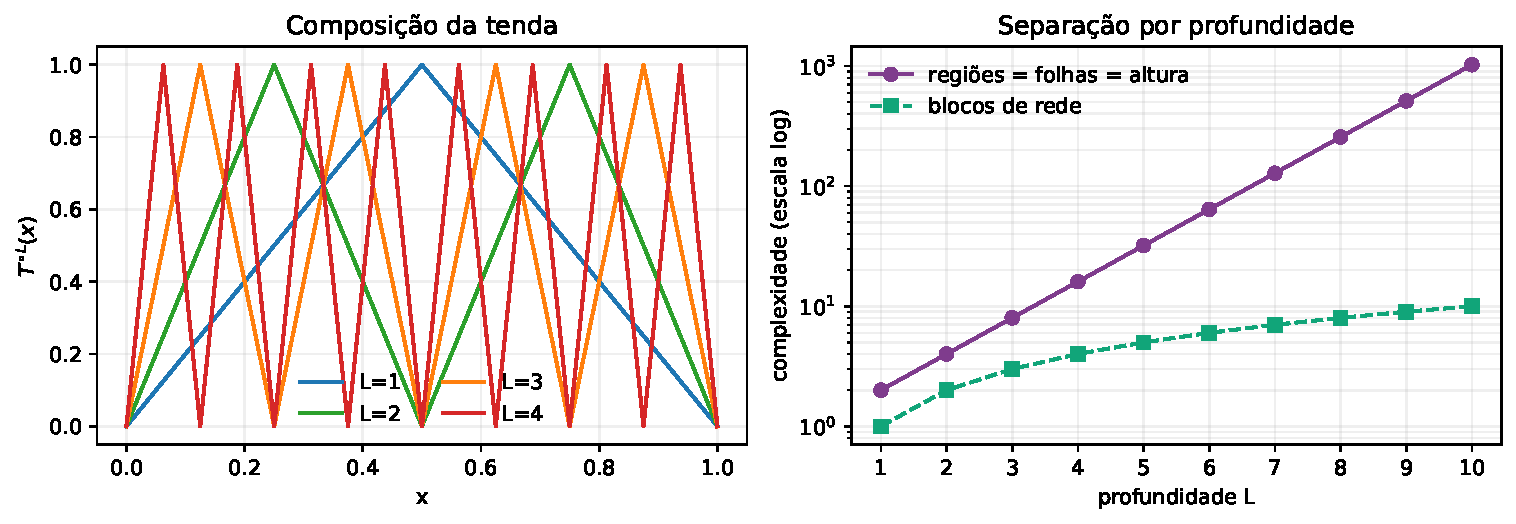
\includegraphics[width=.88\linewidth]{fig_restricoes_rede.pdf}
 \caption{Crescimento dos recursos realizados pela tenda iterada. Os pontos
 provêm de identidades exatas; as linhas apenas guiam a leitura.}
 \label{fig:network-restrictions}
\end{figure}

\begin{table}[t]
 \centering
 \small
 \begin{tabular}{rrrrrr}
\toprule
$M$ & $\varepsilon$ & $D$ & folhas & cota de folhas & erro/$\varepsilon$\\
\midrule
1 & $1/32$ & 12 & 13 & 13 & 0.0099\\
1 & $1/64$ & 13 & 14 & 14 & 0.0037\\
1 & $1/128$ & 14 & 15 & 15 & 0.0131\\
1 & $1/32$ & 11 & 12 & 12 & 0.0245\\
1 & $1/64$ & 12 & 13 & 13 & 0.0099\\
1 & $1/128$ & 13 & 14 & 14 & 0.0120\\
\bottomrule
\end{tabular}

 \caption{Primeiras seis testemunhas da bateria racional de reversão
 aproximada. As redes de entrada possuem quebras não diádicas. O erro é
 calculado exatamente no conjunto unido de quebras, onde o máximo de uma
 diferença linear por partes é atingido; a última coluna arredonda a quatro
 casas as razões exatas do arquivo suplementar.}
 \label{tab:approximate-reverse-audit}
\end{table}

A bateria suplementar fixa $c=1/5$, escolhe de uma a três quebras entre
$\{1/3,2/5,5/7\}$, toma a inclinação inicial em
$(-7/3,-1/2,2/3,5/4)$ e, para $M$ quebras, usa saltos
$a_i=b_{(i+M)\bmod4}$, onde
$(b_0,b_1,b_2,b_3)=(-7/3,-1/2,2/3,5/4)$. Para cada rede são usados
$\varepsilon\in\{1/32,1/64,1/128\}$, totalizando $84$ quantizações. As redes
de entrada, as frações brutas e as razões exatas das seis linhas exibidas
ficam em \path{reproducibility/selecao/resultados_reversibilidade.json}.
Assim, a \cref{tab:approximate-reverse-audit} apresenta testemunhas
reprodutíveis, e não vetores de teste implícitos.

\subsection{A melhor recíproca para o erro bruto}

Todo $g\in\Sigma_N^{\Library,H}$ é $H(N)$-Lipschitz, pois em cada folha sua
inclinação $s$ satisfaz $|s|\le\height(s)\le H(N)$. Consequentemente,
$\omega_2(g,t)_\infty\le2H(N)t$. Essa desigualdade de tipo Bernstein contém
uma recíproca verdadeira, desde que se aceite a perda imposta pelo crescimento
das inclinações. A formulação seguinte não depende da aritmética.

\begin{theorem}[imersão inversa sob crescimento de Lipschitz]
\label{thm:raw-lossy-inverse}
Sejam $\mathcal G_N\subset C([0,1])$ famílias de aproximantes tais que
\begin{equation}
 \operatorname{Lip}(g)\le C_LN^\gamma
 \qquad(g\in\mathcal G_N),
 \qquad \gamma\ge0,
 \label{eq:lipschitz-growth-family}
\end{equation}
e defina
$e_N^{\mathcal G}(f)=\inf_{g\in\mathcal G_N}\|f-g\|_\infty$. Se
\begin{equation}
 A_\alpha(f):=\sup_{N\ge1}N^\alpha e_N^{\mathcal G}(f)<\infty,
 \qquad \alpha>0,
 \label{eq:raw-rate-assumption}
\end{equation}
então, com
\begin{equation}
 \theta_* = \frac{\alpha}{\alpha+\gamma},
 \label{eq:critical-reverse-exponent}
\end{equation}
vale
\begin{equation}
 \omega_2(f,t)_\infty
 \le C_{\alpha,\gamma}(A_\alpha(f)+C_L)t^{\theta_*},
 \qquad 0<t\le\frac12.
 \label{eq:raw-inverse-modulus}
\end{equation}
Consequentemente,
\begin{equation}
 f\in B^{\theta_*}_{\infty,\infty}([0,1])
 \quad\text{e}\quad
 f\in B^\theta_{\infty,r}([0,1])
 \quad(0<\theta<\theta_*,\ 0<r\le\infty).
 \label{eq:raw-inverse-besov}
\end{equation}
\end{theorem}

\begin{proof}
Para qualquer $g\in\mathcal G_N$, a desigualdade triangular para segundas
diferenças e a propriedade Lipschitz dão
\begin{equation}
 \omega_2(f,t)_\infty
 \le4\|f-g\|_\infty+2C_LN^\gamma t.
 \label{eq:inverse-balance}
\end{equation}
Escolha $N$ comparável a $t^{-1/(\alpha+\gamma)}$ e use um aproximante
arbitrariamente próximo do ínfimo. Os dois termos do lado direito passam a
ser $O(t^{\alpha/(\alpha+\gamma)})$, o que prova
\eqref{eq:raw-inverse-modulus}. A caracterização diádica de Besov fornece o
endpoint por supremo. Para $\theta<\theta_*$, a sequência normalizada ganha o
fator geométrico $2^{-j(\theta_*-\theta)}$ e pertence a todo $\ell^r$.
\end{proof}

\begin{corollary}[aplicação às agendas diretas]
\label{cor:raw-library-inverse}
Se $H(N)\le C N^\gamma$, então
\begin{equation}
 \mathscr A_q^\alpha(\Library,H)
 \subset B^{\alpha/(\alpha+\gamma)}_{\infty,\infty}([0,1]),
 \qquad 0<q\le\infty.
 \label{eq:raw-library-inverse}
\end{equation}
Para as agendas $H_{s,0}$ da \cref{sec:direct-height}, isso dá
\begin{equation}
 \mathscr A_q^s(\Library,H_{s,0})
 \subset B^{\vartheta_s}_{\infty,\infty},
 \qquad
 \vartheta_s=
 \begin{cases}
 s/(s+1),&0<s<1,\\
 1/2,&1\le s<2.
 \end{cases}
 \label{eq:corrected-schedule-raw-inverse}
\end{equation}
Se a agenda possui ainda um fator logarítmico, a mesma conclusão vale para
toda ordem estritamente menor que $\vartheta_s$.
\end{corollary}

\begin{proof}
Todo elemento de $\Sigma_N^{\Library,H}$ é $H(N)$-Lipschitz. O funcional com
$q<\infty$ controla o de supremo pela redução diádica do
\cref{thm:dyadic-rate-equivalence}. Um fator logarítmico é dominado por
$N^\eta$ para qualquer $\eta>0$; aplique o teorema com
$\gamma+\eta$ e faça $\eta\downarrow0$.
\end{proof}

O expoente \eqref{eq:critical-reverse-exponent} não é uma folga do balanço.
O \cref{thm:critical-tent-comb} transfere a testemunha para a biblioteca
original, inclusive com a exigência de inclinações locais não nulas.

\begin{theorem}[agudeza por um pente de tendas]
\label{thm:critical-tent-comb}
Fixe $0<\alpha\le\gamma$ e ponha
$\theta_*=\alpha/(\alpha+\gamma)$. Existe
$f\in C([0,1])$ e uma constante $C$ tais que, para a biblioteca original sob
$H(N)=\lceil CN^\gamma\rceil$,
\begin{equation}
 e_N^{\Library,H}(f)\le CN^{-\alpha},
 \label{eq:comb-approximation-rate}
\end{equation}
mas
\begin{equation}
 f\notin B^\theta_{\infty,\infty}\quad(\theta>\theta_*),
 \qquad
 f\notin B^{\theta_*}_{\infty,r}\quad(0<r<\infty).
 \label{eq:comb-sharpness}
\end{equation}
\end{theorem}

\begin{proof}
Escolha um inteiro $J_0$ tão grande que
$J_0(\alpha+\gamma)>3$. Para $j\ge1$, ponha
\[
 a_j=\lceil J_0\alpha j\rceil,
 \qquad b_j=\lfloor J_0\gamma j\rfloor,
 \qquad r_j=a_j+b_j-1.
\]
No intervalo diádico $J_{r_j,1}$, coloque uma tenda $\phi_j$ de altura
$2^{-a_j}$, nula nas extremidades e linear em cada metade. As escolhas
garantem que os suportes são disjuntos e acumulam apenas em $0$. Defina
$f=\sum_{j\ge1}\phi_j$.

A inclinação da $j$-ésima tenda tem módulo $2^{b_j}$ e os valores centrais de
suas duas metades têm altura $2^{a_j+1}$. Seja $T_j$ a árvore diádica em pente
que isola as duas metades das primeiras $j$ tendas. Ela possui
$O(r_j+j)$ folhas; fora dessas tendas, a soma parcial
$f_j=\sum_{i\le j}\phi_i$ é nula em cada folha restante.

Para eliminar todas as inclinações nulas sem alterar o alvo $f$, subdivida uma
vez cada folha plana $J$ de $T_j$ e, sobre $J$, acrescente uma tenda
$\psi_{J,j}$ nula nos extremos e de altura
\[
 \delta_j=2^{-a_{j+1}-2}
\]
no ponto médio. Os suportes dessas pequenas tendas são disjuntos. A função
\[
 g_j=f_j+\sum_{J\ {\rm plano\ em}\ T_j}\psi_{J,j}
\]
é contínua e tem inclinação não nula em toda folha da árvore refinada. Logo
$g_j$ é uma montagem da biblioteca original, não da extensão marcada.

Resta conferir os dois orçamentos. A árvore refinada tem ainda
$O(r_j+j)$ folhas. Em uma folha plana de profundidade $d\le r_j+1$, a nova
inclinação tem módulo $2^{d+1}\delta_j$; sua altura é limitada por
\[
 \max\{2^{a_{j+1}+1},\,2^{r_j-a_{j+1}}\}
 \le C2^{J_0\gamma j}.
\]
Os valores centrais novos têm altura no máximo $2^{a_{j+1}+3}$, e os
parâmetros das tendas originais são limitados por
$C\max\{2^{a_j},2^{b_j}\}$. As células profundas do pente têm índices
$m\in\{0,1,2,3\}$; portanto escala e translação obedecem à mesma cota.
Como $\alpha\le\gamma$, todos esses termos são no máximo
$CN_j^\gamma$ para $N_j=2^{J_0j}$, depois de aumentar $C$. Também
$O(r_j+j)\le N_j$ para $j$ grande; as finitíssimas escalas iniciais são
absorvidas em $C$ e por uma reindexação finita.

Por disjunção dos suportes,
\[
 \|f-g_j\|_\infty
 \le \Bigl\|\sum_{i>j}\phi_i\Bigr\|_\infty+\delta_j
 \le 2^{-a_{j+1}}+\delta_j
 \le C N_j^{-\alpha}.
\]
Para $N_j\le N<N_{j+1}$, use $g_j$; a razão
$N_{j+1}/N_j=2^{J_0}$ é fixa. A monotonicidade da agenda e o ajuste dessa
constante provam \eqref{eq:comb-approximation-rate} para todo $N$.

Se $h_j=2^{-(r_j+1)}$ é a meia-largura da tenda, os valores
$0,2^{-a_j},0$ dão
\[
 \omega_2(f,h_j)_\infty\ge2^{1-a_j}\asymp h_j^{\theta_*}.
\]
Isso exclui toda ordem maior no supremo e torna constante uma subsequência do
coeficiente crítico, que não pertence a nenhum $\ell^r$ finito.
\end{proof}

A exigência $\alpha\le\gamma$ cobre em particular as agendas críticas da
\cref{sec:direct-height}. Ela também expõe por que a informação correta é a inclinação
realizada, não a altura do endereço isoladamente.

\subsection{Funcional de realização: lado direto com altura controlada}

A agudeza do teorema anterior fixa a regularidade determinada pelo erro bruto
e por uma cota de Lipschitz. Para comparar com a suavidade clássica, considere
o funcional de realização associado ao módulo de segunda ordem. Funcionais
desse tipo foram introduzidos para substituir $K$-funcionais degenerados em
aproximação restrita \citep{hristovivanov1990}. Para $N\ge2$, defina
\begin{equation}
 \mathcal R_N^{\Library,H}(f)
 :=\inf_{g\in\Sigma_N^{\Library,H}([0,1])}
 \left\{\|f-g\|_\infty+
 \omega_2(g,N^{-1})_\infty\right\}.
 \label{eq:self-roughness-certificate}
\end{equation}
O primeiro termo mede fidelidade; o segundo impede que uma função com quinas
receba suavidade apenas porque já pertence ao catálogo.

\begin{lemma}[desigualdade inversa universal]
\label{lem:universal-regularized-inverse}
Para toda agenda, toda $f\in C([0,1])$ e todo $N\ge2$,
\begin{equation}
 \frac14\omega_2(f,N^{-1})_\infty
 \le \mathcal R_N^{\Library,H}(f).
 \label{eq:universal-regularized-lower}
\end{equation}
\end{lemma}

\begin{proof}
Para qualquer $g$ admissível,
\[
 \omega_2(f,N^{-1})_\infty
 \le4\|f-g\|_\infty+\omega_2(g,N^{-1})_\infty
 \le4\bigl(\|f-g\|_\infty+\omega_2(g,N^{-1})_\infty\bigr).
\]
Tome o ínfimo.
\end{proof}

\begin{remark}[o que o funcional mede]
\label{rem:realization-functional-scope}
A prova do \cref{lem:universal-regularized-inverse} usa apenas a desigualdade
triangular para segundas diferenças; não usa racionalidade, células diádicas,
altura nem sequer linearidade por partes. Portanto, a direção inversa mede a
suavidade do alvo e vale para qualquer família de candidatos. Ela não é uma
medida específica de aproximabilidade pela biblioteca. O conteúdo específico
deste trabalho é o lado direto: construir, dentro de $\Library$, candidatos
que atingem o majorante com a agenda aritmética explicitada na
\cref{sec:direct-height}.
\end{remark}

\begin{theorem}[Jackson racional para o funcional de realização]
\label{thm:regularized-jackson-bernstein}
Se $0<s<2$ e $f\in B^s_{\infty,\infty}([0,1])$, então, para toda potência de
dois $N$ suficientemente grande e toda altura que satisfaz as hipóteses do
\cref{lem:rational-jackson-height},
\begin{equation}
 \frac14\omega_2(f,N^{-1})_\infty
 \le \mathcal R_N^{\Library,H}(f)
 \le C_0\omega_2(f,N^{-1})_\infty+\frac{C_f}{H(N)},
 \label{eq:two-sided-regularized-equivalence}
\end{equation}
onde $C_0$ é universal e $C_f$ depende apenas de $\|f\|_\infty$ e das
constantes fixadas na racionalização.
Se $\|f\|_{B^s_{\infty,\infty}}^*\le B$, $B\ge1$, e
$H(N)\ge\widehat H_{s,0}^{[B]}(N)$, a mesma estimativa vale para toda potência
diádica $N\ge2$, com $C_f/H(N)$ substituído por $C(B+1)/H(N)$ e constantes
independentes de $f$.
\end{theorem}

\begin{proof}
A cota inferior é o lema anterior. Para a superior, tome o aproximante
racional $g_{N,H}$ do \cref{lem:rational-jackson-height}. Ele satisfaz
\[
 \|f-g_{N,H}\|_\infty
 \le2C_W\omega_2(f,N^{-1})_\infty+C_fH(N)^{-1}.
\]
Além disso, a desigualdade triangular aplicada na direção contrária dá
\[
 \omega_2(g_{N,H},N^{-1})_\infty
 \le\omega_2(f,N^{-1})_\infty+4\|f-g_{N,H}\|_\infty.
\]
Somar as duas estimativas e usar $g_{N,H}$ na definição de
$\mathcal R_N$ prova a cota superior. Na versão sobre a bola, aplique a parte
uniforme do mesmo lema; ela substitui o termo de quantização por
$8(B+1)/H(N)$ em todas as escalas diádicas, e o mesmo cálculo apenas altera a
constante universal.
\end{proof}

Defina o estrato reversível
\begin{equation}
 \mathscr R_q^s(\Library,H)
 :=\left\{f\in C([0,1]):
 \left\|\bigl(2^{rs}\mathcal R_{2^r}^{\Library,H}(f)\bigr)_{r\ge1}
 \right\|_{\ell^q}<\infty\right\}.
 \label{eq:reversible-stratum}
\end{equation}

\begin{theorem}[caracterização pelo funcional de realização]
\label{thm:complete-besov-reversibility}
Para $0<s<2$, valem as igualdades de conjuntos
\begin{align}
 B^s_{\infty,\infty}([0,1])
 &=\mathscr R_\infty^s(\Library,H_{s,0}),
 \label{eq:complete-reverse-endpoint}\\
 B^s_{\infty,q}([0,1])
 &=\mathscr R_q^s(\Library,H_{s,0}),
 &&0<q<\infty,\quad0<s<1,
 \label{eq:complete-reverse-subcritical}\\
 B^s_{\infty,q}([0,1])
 &=\mathscr R_q^s(\Library,H_{s,\kappa}),
 &&0<q<\infty,\quad1\le s<2,\quad\kappa>1/q.
 \label{eq:complete-reverse-critical}
\end{align}
Pode-se substituir a agenda logarítmica da última linha por qualquer agenda
com folga polinomial \eqref{eq:polynomial-slack-schedule}.
\end{theorem}

\begin{proof}
Se o funcional em \eqref{eq:reversible-stratum} é finito, a desigualdade
universal do \cref{lem:universal-regularized-inverse}, na forma
\eqref{eq:universal-regularized-lower}, e a caracterização diádica
\eqref{eq:dyadic-besov-norm} dão imediatamente
$f\in B^s_{\infty,q}$.

Na direção direta, aplique a cota superior. O termo do módulo pertence a
$\ell^q$ pela definição de Besov. Para $s<1$,
\[
 \frac{N^s}{H_{s,0}(N)}=O(N^{s-1}),
\]
que é geometricamente somável nas potências de dois. Para $q=\infty$ e
$s\ge1$, $N^s/H_{s,0}(N)$ é limitado. Para $q<\infty$ e $s\ge1$, a agenda
logarítmica produz $(\log(eN))^{-\kappa}$, cuja subsequência diádica pertence
a $\ell^q$ exatamente sob $\kappa q>1$. A folga polinomial produz
$N^{-\eta}$. Um número finito de escalas iniciais não altera pertinência.
\end{proof}

O dado adicional que torna a taxa reversível é a segunda diferença do próprio
aproximante na escala pareada. A altura permanece aritmética e usa as agendas
da \cref{sec:direct-height}; a uniformidade quantitativa sobre bolas é dada
pelos \cref{thm:direct-besov-height,cor:uniform-besov-ball-embedding}. A igualdade de conjuntos não
deve ser confundida com equivalência de quase-normas do erro bruto.

Para a quina \eqref{eq:reverse-kink}, tomar $g=\psi$ zera o primeiro termo,
mas deixa
\begin{equation}
 \mathcal R_N^{\Library,H}(\psi)
 \le\omega_2(\psi,N^{-1})_\infty=\frac2N.
 \label{eq:kink-regularized-rate}
\end{equation}
A cota universal mostra a mesma ordem. Logo a taxa reversível é exatamente
um, em acordo com \eqref{eq:kink-besov-reverse}, e não infinita.

\begin{table}[t]
 \centering
 \small
 \begin{tabular}{rrrrr}
\toprule
$N$ & $e_N(\psi)$ & $\omega_2(\psi,N^{-1})$ & $N\omega_2$ & $N^{3/2}\omega_2$\\
\midrule
4 & 0 & $1/2$ & 2.000 & 4.000\\
8 & 0 & $1/4$ & 2.000 & 5.657\\
16 & 0 & $1/8$ & 2.000 & 8.000\\
32 & 0 & $1/16$ & 2.000 & 11.314\\
64 & 0 & $1/32$ & 2.000 & 16.000\\
128 & 0 & $1/64$ & 2.000 & 22.627\\
\bottomrule
\end{tabular}

 \caption{A quina sob o erro bruto e a parcela de autorregularidade obtida
 com o candidato $g=\psi$. Embora $e_N(\psi)=0$, essa parcela é $2/N$; a
 cota universal \eqref{eq:universal-regularized-lower} garante que o ínfimo
 completo tem a mesma ordem $N^{-1}$.}
 \label{tab:kink-regularized-certificate}
\end{table}

A \cref{tab:kink-regularized-certificate} torna explícita a diferença entre
erro bruto nulo e autorregularidade de ordem $N^{-1}$.

\subsection{Estabilidade da caracterização ao ampliar a arquitetura}

O certificado é definido no espaço de funções, independentemente de uma
parametrização neural, o que permite comparar famílias arquiteturais inteiras.

\begin{theorem}[reversibilidade estável por inclusão de redes]
\label{thm:architecture-stable-reversibility}
Seja $(\mathcal N_N)$ qualquer família de funções realizadas por redes ReLU
aninhada no orçamento, isto é,
\begin{equation}
 0\in\mathcal N_N,
 \qquad \mathcal N_N\subseteq\mathcal N_{N+1}
 \qquad(N\ge1),
 \label{eq:network-family-nesting}
\end{equation}
e suponha que, para alguma constante $c\ge1$,
\begin{equation}
 \Sigma_N^{\Library,H}([0,1])\subseteq\mathcal N_{\lceil cN\rceil}
 \qquad(N\ge1).
 \label{eq:network-family-contains-library}
\end{equation}
Defina
\begin{equation}
 \mathcal R_N^{\mathcal N}(f)
 =\inf_{R\in\mathcal N_N}
 \left\{\|f-R\|_\infty+\omega_2(R,N^{-1})_\infty\right\}.
 \label{eq:network-regularized-certificate}
\end{equation}
Sob cada uma das agendas do
\cref{thm:complete-besov-reversibility}, substituir
$\mathcal R_N^{\Library,H}$ por $\mathcal R_N^{\mathcal N}$ preserva as
igualdades \eqref{eq:complete-reverse-endpoint}--
\eqref{eq:complete-reverse-critical}.
\end{theorem}

\begin{proof}
A desigualdade inversa
\[
 \omega_2(f,N^{-1})_\infty\le4\mathcal R_N^{\mathcal N}(f)
\]
vale para toda função contínua $R$, independentemente da arquitetura. Essa é
a inclusão do estrato neural no Besov. Na direção direta, realize na família
neural o aproximante racional da
\cref{thm:regularized-jackson-bernstein}. Ponha
$d=2^{\lceil\log_2c\rceil}$. Para todo orçamento diádico $M=2^r\ge d$, o
número $n=M/d$ é também uma potência de dois e
$\lceil cn\rceil\le M$. Por \eqref{eq:network-family-contains-library} e pelo
aninhamento \eqref{eq:network-family-nesting},
\[
 \Sigma_n^{\Library,H}([0,1])
 \subseteq\mathcal N_{\lceil cn\rceil}
 \subseteq\mathcal N_M.
\]
Se $g_{n,H}$ é o aproximante usado naquele teorema, a monotonicidade do módulo
na escala fornece
\begin{align*}
 \mathcal R_M^{\mathcal N}(f)
 &\le \|f-g_{n,H}\|_\infty+\omega_2(g_{n,H},M^{-1})_\infty\\
 &\le \|f-g_{n,H}\|_\infty+\omega_2(g_{n,H},n^{-1})_\infty\\
 &\le C_0\omega_2(f,n^{-1})_\infty+\frac{C_f}{H(n)}.
\end{align*}
Como $M=dn$, multiplicar por $M^s$ introduz apenas o fator fixo $d^s$, e a
passagem de $M$ a $n$ desloca por $\log_2d$ índices as sequências diádicas.
As mesmas estimativas de $\ell^q$ da
\cref{thm:complete-besov-reversibility} concluem a direção direta. Um número
finito de escalas $M<d$ não afeta o estrato.
\end{proof}

O \cref{thm:architecture-stable-reversibility} explica por que a profundidade deixa de ser uma ameaça lógica à
recíproca. Uma rede profunda pode representar a tenda iterada com poucos
blocos, mas sua segunda diferença na escala pareada não desaparece. Adicionar
tais redes ao conjunto de candidatos pode reduzir o erro de aproximação, mas
não pode reduzir o certificado abaixo de um quarto do módulo do alvo.

\begin{figure}[t]
 \centering
 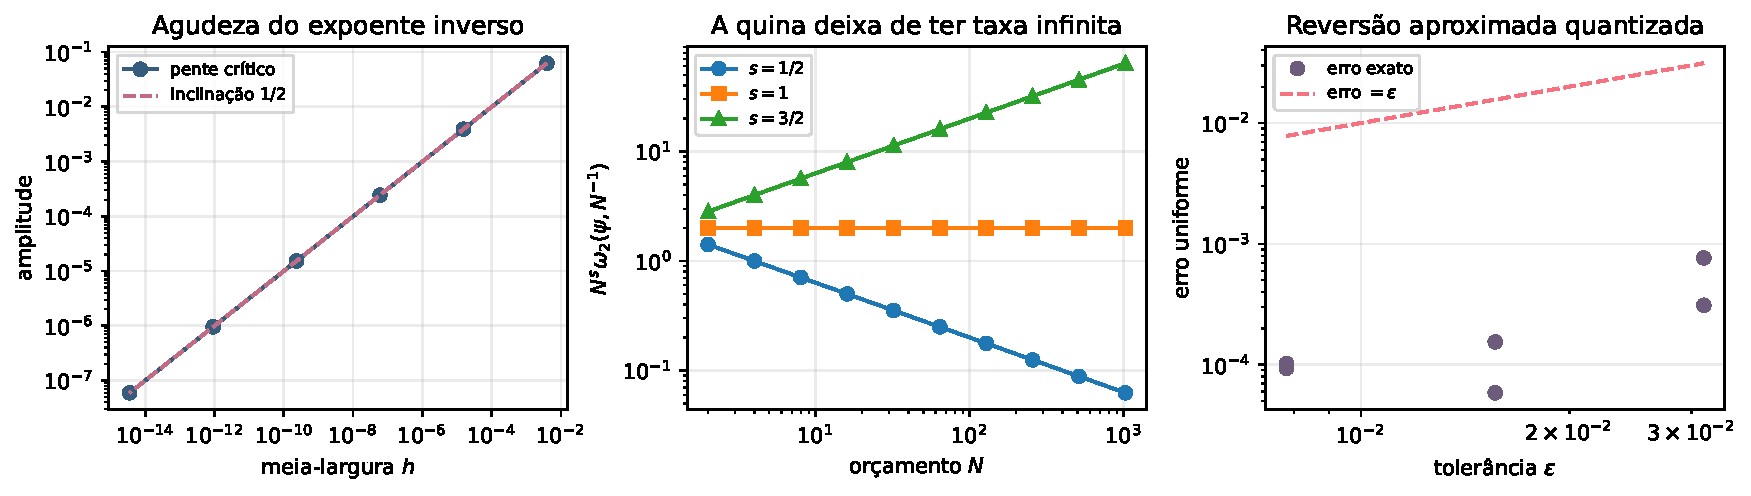
\includegraphics[width=.98\linewidth]{fig_reversibilidade_regularizada.pdf}
 \caption{Três diagnósticos da reversibilidade. À esquerda, o pente de tendas
 realiza o expoente crítico $\alpha/(\alpha+\gamma)$. Ao centro, o certificado
 atribui à quina exatamente a ordem um. À direita, a quantização de redes com
 quebras não diádicas permanece abaixo da tolerância prescrita.}
 \label{fig:regularized-reversibility}
\end{figure}

Os três mecanismos aparecem lado a lado na
\cref{fig:regularized-reversibility}; a coluna relativa ao pente usa agora a
construção na biblioteca original do \cref{thm:critical-tent-comb}.

\subsection{Validação executável}

O programa \texttt{reversibilidade\_regularizada.py} executa uma auditoria
independente em aritmética \texttt{Fraction}. Ele:
\begin{enumerate}[label=(\roman*),leftmargin=2.2em]
 \item executa $2952$ idas e voltas exatas entre formas hinge e árvores
 canônicas, das quais $1160$ contêm ao menos uma região plana;
 \item verifica em todos os casos as duas cotas de folhas de
 \eqref{eq:canonical-tree-leaf-bounds};
 \item quantiza $84$ redes com quebras não diádicas e confere exatamente erro,
 número de folhas, inclinações não nulas e altura;
 \item testa $1260$ instâncias da desigualdade universal que sustenta
 \eqref{eq:universal-regularized-lower};
 \item reproduz a quina em dez escalas, a tenda profunda até $1024$ regiões e
 seis níveis do pente crítico, verificando em cada nível a perturbação, o erro,
 a altura, o número de folhas e a ausência de inclinações nulas na biblioteca
 original.
\end{enumerate}

A reversibilidade assume três formas. A biblioteca $\Library$ corresponde
exatamente à imagem rasa caracterizada por dados racionais, nós diádicos e
inclinações não nulas. A extensão marcada inclui regiões planas e produz uma
bijeção funcional rasa. Redes reais genéricas admitem aproximações inversas
com recursos explícitos. No nível de classes funcionais, o erro bruto possui a recíproca com perda do
\cref{thm:raw-lossy-inverse}, enquanto o certificado
\eqref{eq:self-roughness-certificate} fornece a caracterização direta e
inversa completa do \cref{thm:complete-besov-reversibility}. Essas três formas
separam representação exata, quantização e regularidade funcional.

\FloatBarrier
\section{Verificação computacional reproduzível}
\label{sec:verification}

Os experimentos são determinísticos. O script \path{compilar.sh} coordena seis
programas: \path{reproduzir_curvas.py} e os cinco programas de
\path{reproducibility/selecao/}. Os arquivos JSON correspondentes registram os
testes e os valores tabulados. O arquivo
\path{reproducibility/biblioteca/resultados.json} registra também as versões
efetivamente usadas. Na execução de referência que acompanha este manuscrito:
Python 3.12.13, NumPy 2.3.5 e Matplotlib 3.10.8. A auditoria independente
também executou as seis suítes com Python 3.10.12; por isso, o requisito do
pacote é Python 3.10 ou posterior.

\subsection{Indexação}

Foram verificados:
\begin{itemize}[leftmargin=1.6em]
 \item $\pi(\pi^{-1}(n))=n$ e a ida e volta da descompactação quádrupla para $0\le n<20,000$;
 \item unicidade dos primeiros $5,000$ termos de $Q$ e $Q^{\!*}$, ausência de zero na segunda enumeração e a desigualdade de posto $j<3\height(Q(j))^2$ em ambas;
 \item $CW(2^{q-1})=1/q$ para $1\le q\le20$.
\end{itemize}
Esses testes auditam computacionalmente as identidades demonstradas.

\subsection{Conversão ReLU e minimização em catálogos finitos}

As rotinas públicas \texttt{assembly\_to\_relu} e
\texttt{relu\_to\_assembly} implementam as duas direções do
\cref{thm:assembly-relu}. Foram geradas deterministicamente $4.096$ montagens
racionais, com duas a sete folhas. Em aritmética
\texttt{fractions.\allowbreak Fraction}, o script verificou exatamente, em cada folha, os
valores nos dois extremos e no centro, a inclinação local, a largura
$N-1$ da rede e a igualdade da assinatura linear por partes após a conversão
inversa. Não há tolerância de ponto flutuante nesses testes.

O \cref{alg:finite-enumeration} foi executado sobre a raiz
$K=J_{0,0}=[0,1]$. O funcional de teste também é exato:
\begin{equation}
 \mathcal J(g)=\sum_{x\in\{0,1/4,1/2,3/4,1\}}
 \bigl(g(x)-2|x-1/2|\bigr)^2.
 \label{eq:catalog-test-objective}
\end{equation}
Cada caso foi enumerado uma segunda vez com a ordem de árvores e átomos
invertida. O conjunto de funções, a menor representação de cada função, o
valor mínimo e o fluxo vencedor permaneceram idênticos.

A \cref{tab:catalogos-pt} reúne as cardinalidades, as redundâncias de
representação e os minimizadores exatos dessas instâncias.

\begin{table}[t]
\centering
\caption{Enumeração e minimização exatas em
$\Sigma_{D,H}^{\Library}([0,1])$.}
\label{tab:catalogos-pt}
\small
\begin{tabular}{rrrrrr}
\toprule
$D$ & $H$ & representações & funções & $\min J$ & bits do desempate\\
\midrule
0 & 2 & 42 & 42 & $\frac{29}{32}$ & 12\\
1 & 2 & 102 & 96 & $0$ & 33\\
2 & 2 & 102 & 96 & $0$ & 33\\
0 & 3 & 210 & 210 & $\frac{19}{24}$ & 18\\
\bottomrule
\end{tabular}

\end{table}

A coluna ``representações'' é maior que a coluna ``funções'' quando árvores
redundantes avaliam no mesmo objeto; o desempate é feito somente depois dessa
deduplicação funcional. O salto de $D=0$ para $D=1$, $H=2$, inclui a montagem
em V que realiza exatamente o alvo de \eqref{eq:catalog-test-objective}. Já
$D=2$, $H=2$, não acrescenta folhas de escala $k=2$, pois sua altura atômica é
pelo menos $3$. O script verifica ainda as inclusões de
\eqref{eq:catalog-nesting} e a monotonicidade dos valores mínimos.

\subsection{Roundtrip dos formatos de codificação}

Os codificadores de \cref{subsec:coding-formats} e seus decodificadores foram
executados nas mesmas $4.096$ montagens racionais usadas no teste ReLU. Em
todos os casos, o fluxo atômico recuperou a assinatura linear por partes e os
dois fluxos ReLU recuperaram exatamente cada \texttt{Fraction} da rede. Foram
também verificadas, parâmetro a parâmetro, as cotas
\eqref{eq:slope-jump-height}--\eqref{eq:intercept-height}.

A fatia $N=2$ da família de \eqref{eq:coding-gap-family} permite comparar os
comprimentos sem regressão nem ajuste assintótico. A
\cref{tab:codificacoes-pt} dá os valores exatos e a
\cref{fig:codificacoes-pt} mostra as ordens de crescimento:
\begin{table}[t]
\centering
\caption{Comprimentos exatos dos três fluxos prefix-free na família crítica.}
\label{tab:codificacoes-pt}
\small
\begin{tabular}{rrrrr}
\toprule
$H$ & $L_{\rm atom}$ & $L_{\rm ReLU,str}$ & $L_{\rm ReLU,rat}$ & razão rat./str.\\
\midrule
4 & 29 & 31 & 35 & 1.129\\
8 & 33 & 35 & 51 & 1.457\\
16 & 37 & 39 & 83 & 2.128\\
32 & 41 & 43 & 147 & 3.419\\
64 & 45 & 47 & 275 & 5.851\\
128 & 49 & 51 & 531 & 10.412\\
\bottomrule
\end{tabular}

\end{table}

\begin{figure}[t]
 \centering
 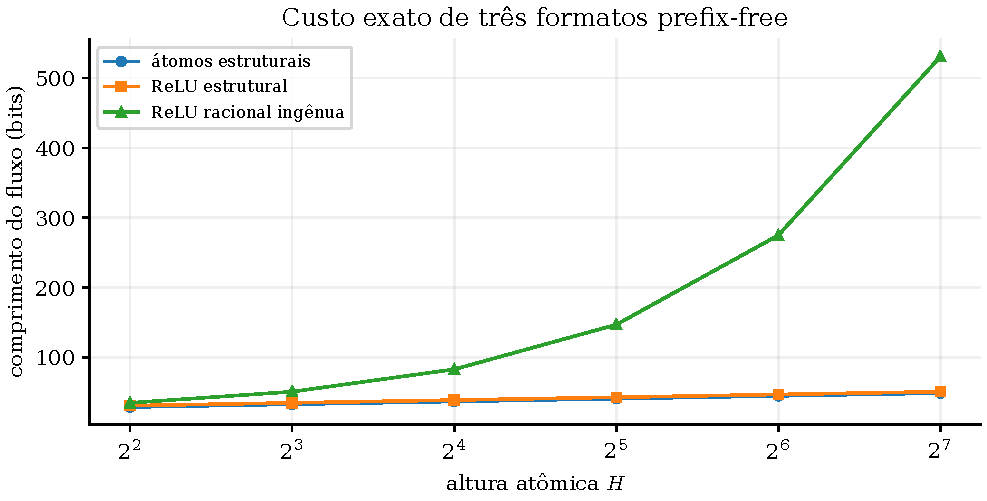
\includegraphics[width=.82\linewidth]{fig08_codificacoes.pdf}
 \caption{O par diádico estrutural mantém o custo logarítmico; expandir o
 denominador $2^k$ como parte de uma fração racional produz a sobrecarga
 linear prevista pelo \cref{thm:coding-formats}.}
 \label{fig:codificacoes-pt}
\end{figure}

\subsection{Orçamento conjunto de folhas, altura e bits}

A construção do \cref{thm:joint-budget} foi executada integralmente em
aritmética \texttt{Fraction} para $N=2,4,\ldots,256$ e quatro funções
racionais da bola $\mathcal F_{1,8}$: quadrática, constante, afim e racional
sem polo. Ao todo foram inspecionadas $2.040$ folhas. O script verificou,
sem tolerância numérica, continuidade, inclinações não nulas, erro nodal no
máximo $1/(2N^2)$, a cota $\height_{\max}\le18N^2$ e as cotas individuais
para intercepto, nós, inclinação inicial e saltos ReLU. Os três fluxos foram
decodificados de volta em cada escala.

Na sonda quadrática $f_\star(x)=4x(x-1)$, o erro uniforme foi maximizado
exatamente nos extremos e no único ponto crítico de cada folha. Isso produz
as frações da \cref{tab:joint-budget-pt}; em todas as linhas,
$N^2\|f_\star-g_N\|_\infty=49/64$, enquanto o certificado do teorema é
$3/2$ na mesma normalização (equivalentemente,
$\|f_\star-g_N\|_\infty\le3/(2N^2)$ antes de multiplicar por $N^2$). A
constância observada constitui uma regressão exata da
implementação da grade alternada.

\subsection{Cota uniforme para a exponencial}

Para $f(x)=e^x$, o máximo do erro em uma célula $[x_L,x_R]$ ocorre no ponto crítico exato
\[
 e^{x_*}=\frac{e^{x_R}-e^{x_L}}{x_R-x_L}.
\]
Isso permite calcular a \cref{tab:exp-pt} sem amostragem. A razão erro/cota converge a $1$, como previsto pelo \cref{thm:uniform}.

\subsection{Validação da aritmética intervalar}

A rotina \texttt{BoundSecondDerivative(...)} foi testada em polinômio, função
racional, $\exp$, $\sin$, composição com $\cos$ e função de Runge. Todos os
extremos produzidos são racionais; para $x^2$, o 2-jato retorna exatamente
$[2,2]$. A tentativa de certificar $1/x$ em $[-1,1]$ termina com falha segura,
pois nenhuma subdivisão finita separa o denominador de zero. Para Runge, a
subdivisão reduz o majorante e o intervalo final contém a curvatura exata
$50$.

Para tornar inequívoca a função de cada número, a \cref{tab:intervalos-pt}
distingue erro amostrado, certificado e valor exato quando este está
disponível.
\begin{table}[t]
\centering
\caption{Três níveis de validação; somente $e_{\rm cert}$ sustenta uma
garantia quando $e_{\rm exato}$ não é conhecido.}
\label{tab:intervalos-pt}
\small
\begin{tabular}{lrrrr}
\toprule
função e intervalo & $e_{\rm emp}$ & $e_{\rm cert}$ & $e_{\rm exato}$ & $e_{\rm cert}/e_{\rm exato}$\\
\midrule
$x^2$, $[0,1]$ & $2.500\,10^{-1}$ & $2.500\,10^{-1}$ & $2.500\,10^{-1}$ & $1.000$\\
$e^x$, $[0,1]$ & $2.119\,10^{-1}$ & $3.398\,10^{-1}$ & $2.119\,10^{-1}$ & $1.604$\\
Runge, $[-1,1]$ & $9.615\,10^{-1}$ & $2.500\,10^{1}$ & $9.615\,10^{-1}$ & $26.000$\\
\bottomrule
\end{tabular}

\end{table}
Os $20.001$ pontos usados por expressão verificam regressões de implementação
e medem a folga. A inclusão da \cref{prop:interval-majorant} decorre da
aritmética intervalar racional.

\subsection{Refinamento certificado da função de Runge}

Para
\begin{equation}
 f(x)=\frac{1}{1+25x^2},\qquad
 f''(x)=\frac{50(75x^2-1)}{(1+25x^2)^3},
 \label{eq:runge}
\end{equation}
o algoritmo adaptativo usa o majorante intervalar de
\eqref{eq:interval-majorant}. O máximo analítico abaixo é mantido apenas como
referência independente para medir a folga do certificado.

\begin{lemma}[majorante local da função de Runge]\label{lem:runge-majorant}
Em todo intervalo fechado $J\subset[-1,1]$, o máximo de $|f''|$ é atingido em um extremo de $J$ ou em um ponto de $\{0,-0{,}2,0{,}2\}\cap J$.
\end{lemma}

\begin{proof}
Derivando \eqref{eq:runge},
\[
 f'''(x)=\frac{7500x(2-50x^2)}{(1+25x^2)^4},
\]
cujos únicos zeros são $0$ e $\pm0{,}2$. Um máximo interior não nulo de $|f''|$ deve ser ponto crítico de $f''$; os zeros de $f''$ têm módulo zero e não introduzem máximos positivos. Restam os três pontos críticos e os extremos do intervalo.
\end{proof}

A \cref{tab:adaptive-pt} separa o erro empírico, o certificado intervalar e
a referência de curvatura exata em cada tolerância.

\begin{table}[t]
\centering
\caption{Refinamento adaptativo com majorante intervalar para
\eqref{eq:runge}. A coluna ``cert. $M$ exato'' usa o
\cref{lem:runge-majorant} somente como referência.}
\label{tab:adaptive-pt}
\scriptsize
\begin{tabular}{rrrrrrr}
\toprule
$\varepsilon_I$ & folhas & $e_{\rm cert}$ & $e_{\rm emp}$ & cert. $M$ exato & folga & uniforme\\
\midrule
$2.000\,10^{-2}$ & 20 & $1.939\,10^{-2}$ & $9.390\,10^{-3}$ & $1.819\,10^{-2}$ & $1.066$ & 64\\
$1.000\,10^{-2}$ & 26 & $6.468\,10^{-3}$ & $5.921\,10^{-3}$ & $6.104\,10^{-3}$ & $1.060$ & 64\\
$5.000\,10^{-3}$ & 36 & $4.908\,10^{-3}$ & $3.190\,10^{-3}$ & $4.708\,10^{-3}$ & $1.042$ & 128\\
$2.500\,10^{-3}$ & 46 & $2.272\,10^{-3}$ & $1.619\,10^{-3}$ & $2.215\,10^{-3}$ & $1.026$ & 128\\
$1.250\,10^{-3}$ & 66 & $1.202\,10^{-3}$ & $1.042\,10^{-3}$ & $1.177\,10^{-3}$ & $1.021$ & 256\\
$6.250\,10^{-4}$ & 88 & $5.608\,10^{-4}$ & $4.707\,10^{-4}$ & $5.537\,10^{-4}$ & $1.013$ & 256\\
$3.125\,10^{-4}$ & 126 & $3.100\,10^{-4}$ & $2.870\,10^{-4}$ & $3.037\,10^{-4}$ & $1.021$ & 512\\
\bottomrule
\end{tabular}

\end{table}

O erro $e_{\rm emp}$ foi avaliado em $4.001$ pontos por folha; a garantia vem
de $e_{\rm cert}$, calculado exclusivamente com extremos racionais, precisão
$P=96$ bits e $32$ subcaixas por folha. A coluna de referência substitui o
majorante intervalar pelo máximo analítico do \cref{lem:runge-majorant}; a
razão entre as duas é a folga, não um fator usado na garantia. Para uma malha
uniforme com $N$ segmentos em $[-1,1]$, o valor exato
$\|f''\|_\infty=50$ dá certificado $25/N^2$; a última coluna mostra a menor
potência de dois que o torna menor que $\varepsilon_I$.

O arquivo \texttt{resultados.json} registra também
\texttt{scaled\_leaf\_count\_sqrt\_tolerance}$=\sqrt{\varepsilon_I}N(\varepsilon_I)$
em cada linha. Essa quantidade é diagnóstica: a
\cref{prop:adaptive-dyadic-oscillation} mostra que, mesmo no caso de curvatura
constante, ela oscila entre dois limites separados por um fator dois. Nenhuma
convergência à constante de nós livres é inferida desses valores.

A \cref{fig:adaptive-pt} compara a malha adaptativa certificada com a uniforme
e mostra uma das partições produzidas.

\begin{figure}[t]
 \centering
 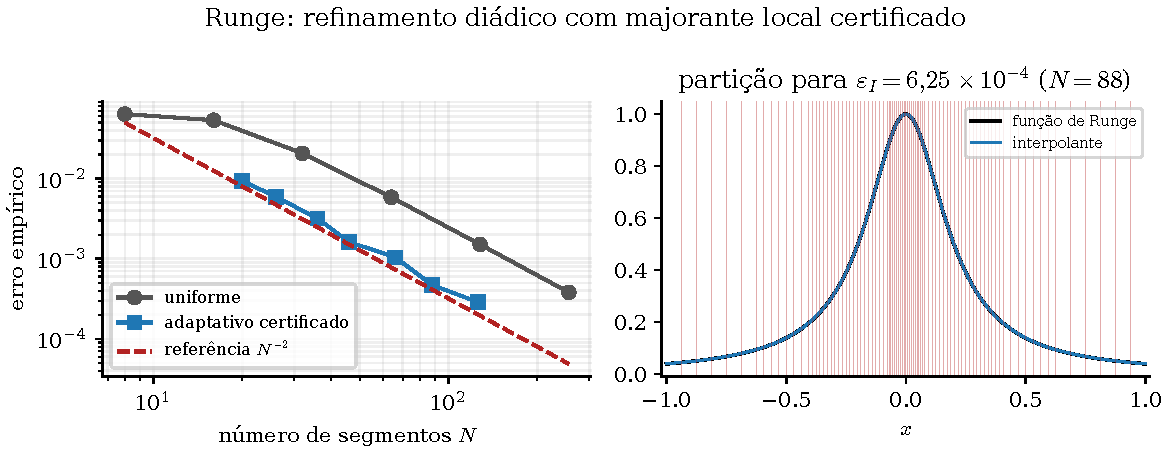
\includegraphics[width=.94\linewidth]{fig05_adaptativo.pdf}
 \caption{Erro empírico e partição adaptativa. A prova da garantia usa o majorante local, não a curva amostrada.}
 \label{fig:adaptive-pt}
\end{figure}

\subsection{Restrição de curvatura e codebook sem fator logarítmico}

A melhoria de \eqref{eq:code-length} não vem de trocar os átomos nem as grades:
vem de contar o codebook com a restrição de diferença segunda em vez de contar
livremente os vetores da grade. Como a afirmação é sobre uma constante
universal, ela é verificável.

O script avalia quatro sondas determinísticas, cada uma reescalada pelo fator
$\min\{R/\|f\|_\infty,\,M/\|f''\|_\infty\}$ para que pertença de fato a
$\mathcal F_{R,M}$ com $R=1$ e $M=8$: a quadrática que satura as duas
restrições simultaneamente, dois harmônicos e a função de Runge reescalada.
Sem esse reescalamento a sonda de Runge teria $\|f''\|_\infty=200$ e ficaria
fora da bola, tornando o teste vazio. Para cada tolerância, verifica-se que
$\varepsilon/2<\delta\le\varepsilon$, que $Mh^2\le4\varepsilon$, que o erro
nodal não excede $\delta/2$, que valores adjacentes são distintos, que cada
peça é um átomo de inclinação racional não nula e que a distorção fica dentro
de $\varepsilon$.

\begin{table}[t]
\centering
\caption{Sucessores admissíveis por nó e comprimento do índice global reescalado.}
\label{tab:codebook-pt}
\small
\begin{tabular}{rrrrrr}
\toprule
$\varepsilon$ & $N$ & sucessores & distorção & $L_\varepsilon^{\mathrm{global}}\sqrt{\varepsilon}$ & antigo $\cdot\sqrt{\varepsilon}$\\
\midrule
$6{,}250\,10^{-2}$ & 8   & 9 & $3{,}90\,10^{-2}$ & $10{,}68$ & $13{,}50$\\
$1{,}562\,10^{-2}$ & 16  & 9 & $9{,}68\,10^{-3}$ & $10{,}34$ & $17{,}00$\\
$3{,}906\,10^{-3}$ & 32  & 9 & $2{,}26\,10^{-3}$ & $10{,}00$ & $20{,}62$\\
$9{,}766\,10^{-4}$ & 64  & 9 & $6{,}98\,10^{-4}$ & $9{,}74$  & $24{,}38$\\
$2{,}441\,10^{-4}$ & 128 & 9 & $1{,}62\,10^{-4}$ & $9{,}56$  & $28{,}22$\\
\bottomrule
\end{tabular}
\end{table}

A \cref{tab:codebook-pt} mostra o essencial. O número de sucessores
admissíveis por nó, dados os dois valores anteriores, é $9$ em todas as
tolerâncias --- abaixo da constante $K=25$ usada na demonstração, que é
portanto conservadora e não ajustada aos dados. As duas últimas colunas são o
diagnóstico do fator logarítmico: o comprimento do índice global da cota atual,
multiplicado por $\sqrt{\varepsilon}$, permanece limitado e até decresce
levemente, enquanto a contagem termo a termo de cada nó cresce
como $\log(1/\varepsilon)$ na mesma normalização. É exatamente a diferença
entre $O(\varepsilon^{-1/2})$ e $O(\varepsilon^{-1/2}\log(1/\varepsilon))$.

\subsection{Contagem de átomos e otimalidade minimax do endereço}

A \cref{tab:enderecos-pt} confronta a contagem exata $|\Library_H|$ com as cotas do
\cref{lem:atom-count} e compara, no pior caso sobre $\Library_H$, o endereço
aritmético $n$ do gerador $\Gamma$ com o endereço $n^\sharp$ da enumeração por
altura da \cref{def:sharp}. A coluna final registra a cota inferior universal,
quanto ao endereçamento sob o calibre fixado, do
\cref{thm:address-lower}. Os expoentes empíricos, obtidos por regressão de
$\log_2(\cdot)$ contra $\log_2H$ nas últimas linhas, aproximam $6$ para
$|\Library_H|$ e $n^\sharp$ e $8$ para $n$, como previsto.

\begin{table}[t]
\centering
\caption{Contagem de átomos por altura e comprimento de endereço no pior caso.}
\label{tab:enderecos-pt}
\small
\begin{tabular}{rrrrr}
\toprule
$H$ & $|\Library_H|$ & $|\Library_H|/(18H^6)$ & $\max n$ ($\Gamma$) & $\max n^\sharp=$ cota inf.\\
\midrule
2 & 252 & 0.2188 & 3231 & 251\\
3 & 3150 & 0.2401 & 87127 & 3149\\
4 & 14168 & 0.1922 & 519638 & 14167\\
6 & 142692 & 0.1699 & 9515572 & 142691\\
8 & 897840 & 0.1903 & 113062957 & 897839\\
12 & 9192456 & 0.1710 & 2233224112 & 9192455\\
16 & 50315232 & 0.1666 & 20668188575 & 50315231\\
24 & 582320976 & 0.1693 & 534070940833 & 582320975\\
32 & 3378271680 & 0.1748 & 5622328883731 & 3378271679\\
48 & 36947682720 & 0.1678 & 131374552971847 & 36947682719\\
64 & 206341325696 & 0.1668 & 1289353431661883 & 206341325695\\
\bottomrule
\end{tabular}

\end{table}

A \cref{fig:enderecos-pt} torna visível a diferença entre os expoentes do
gerador aritmético e da enumeração por cascas, sempre para o calibre
\eqref{eq:atom-height}.

\begin{figure}[t]
 \centering
 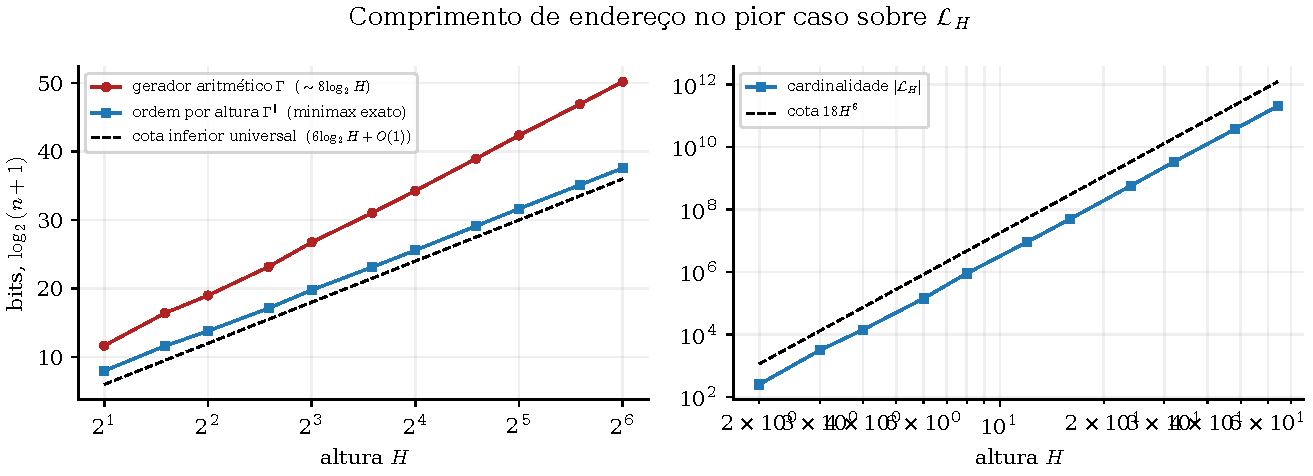
\includegraphics[width=.92\linewidth]{fig06_enderecos.pdf}
 \caption{Comprimento de endereço no pior caso sobre $\Library_H$. A enumeração
 por altura $\Gamma^\sharp$ acompanha a cota inferior relativa a $\Library_H$ com uma folga
 limitada; o gerador aritmético $\Gamma$ paga um fator constante $4/3$ no
 expoente em troca de inversa em forma fechada.}
 \label{fig:enderecos-pt}
\end{figure}

Foi ainda verificada, para $0\le n^\sharp<20{,}000$, a bijetividade de
$\Gamma^\sharp$ nos dois sentidos e a coincidência dos conjuntos
$\Gamma(\{0,\ldots,N\})$ e $\Gamma^\sharp(\{0,\ldots,N'\})$ quando restritos a
uma mesma casca de altura.

\section{Conclusão}
\label{sec:conclusion}

A biblioteca construída combina uma enumeração invertível, montagens densas,
serializações executáveis e aproximação sob orçamento aritmético. A inclinação
não nula torna o suporte recuperável pela interface global; por isso
$\Gamma$ conserva a semântica operacional, enquanto $\Gamma^\sharp$ atua como
codec minimax sem alterar a função selecionada. Sob o calibre fixado, a
contagem $\Theta(H^6)$, o pior índice $\Theta(H^8)$ do gerador aritmético e os
três formatos prefix-free distinguem cardinalidade, endereço e comprimento de
descrição.

Em bolas limitadas de $C^2$, a construção racional alcança simultaneamente
erro $O(N^{-2})$, uma agenda suficiente de altura $O(N^2)$ e
$O(N\log N)$ bits. O refinamento adaptativo
é certificado por aritmética intervalar com falha segura. Para classes de
Besov, a dependência do limiar foi rastreada até a norma do alvo, produzindo
agendas uniformes sobre bolas e estimativas quantitativas sem um
$n_0$ dependente da função. Como o funcional de taxa bruto não é homogêneo
sobre escalares reais, essas estimativas são corretamente formuladas como
controle uniforme de bolas, e não como uma quase-norma inexistente.

A restrição estritamente diádica produz um fenômeno quantitativo próprio: o
envelope assintótico $[I(f)^2/8,I(f)^2/2]$, a lei exata de curvatura constante
e as fases periódicas de quadráticas por partes. Para o erro bruto sob
crescimento Lipschitz $N^\gamma$ e na faixa $0<\alpha\le\gamma$, a ordem inversa
$\alpha/(\alpha+\gamma)$ é aguda já na biblioteca original; a perturbação
diádica introduzida no pente de tendas remove todas as regiões planas sem
alterar a função-alvo nem os expoentes de folhas, altura e erro.

O funcional que soma erro e segunda diferença do aproximante é um funcional
de realização clássico. Sua desigualdade inversa é universal e mede suavidade,
não aproximabilidade específica pela biblioteca. O resultado próprio é o lado
direto de Jackson com inclinações racionais não nulas e agendas explícitas de
altura; a caracterização continua válida em uma família ReLU aninhada no
orçamento que contenha as montagens após reindexação linear.

O bloco de programação dinâmica é mantido como teoria auxiliar de exatidão:
pares de fronteira são estados suficientes, a truncagem torna o catálogo
finito e a cota de bits agora acompanha o crescimento dos operandos racionais.
As instâncias computacionais verificam essas identidades e não são tratadas
como benchmark. Para publicação, o documento-sistema admite a decomposição em
três peças --- constantes diádicas; endereçamento e codificação; estratos de
altura e teoremas inversos --- com esse bloco algorítmico como apêndice. O
documento unificado permanece útil para conservar as conexões transversais.

Permanecem abertas a constante assintótica do melhor aproximante racional sob
uma agenda fixa de altura e a descrição do conjunto de acumulação para
curvaturas variáveis além do envelope universal. Depósitos públicos com DOI,
ORCID e declarações autorais definitivas exigem informações ou ações externas
e, por isso, são registrados no pacote como pendências explícitas, não como
dados inferidos.

\section*{Declarações editoriais}
\addcontentsline{toc}{section}{Declarações editoriais}

\noindent\textbf{Agradecimentos.}
Não foram informados agradecimentos adicionais no material fornecido pelo
autor.

\medskip
\noindent\textbf{Financiamento.}
Informação não fornecida. Antes de qualquer submissão, o autor deve confirmar
expressamente se o trabalho recebeu financiamento e, em caso positivo,
informar agência, processo e beneficiário.

\medskip
\noindent\textbf{Conflitos de interesse.}
Informação não fornecida. A declaração definitiva depende de confirmação
expressa do autor e não foi inferida nesta revisão.

\medskip
\noindent\textbf{Disponibilidade de dados e código.}
Todos os dados sintéticos, scripts, arquivos JSON, tabelas geradas e instruções
necessários para reproduzir os resultados computacionais acompanham o pacote
desta versão. Ainda não foi fornecido um identificador persistente de
repositório; o DOI deverá substituir esta frase após o depósito público.

\medskip
\noindent\textbf{ORCID.}
Não informado. Nenhum identificador foi atribuído ou inferido.

\medskip
\noindent\textbf{Nota biográfica.}
Victor Gabriel de Oliveira é pesquisador independente no Brasil. Informações
biográficas adicionais não foram fornecidas.


\appendix
\section{Quadro de notação}
\label{app:notation}

\begin{longtable}{@{}>{\raggedright\arraybackslash}p{.27\linewidth}>{\raggedright\arraybackslash}p{.68\linewidth}@{}}
\toprule
Símbolo & Significado\\
\midrule
\endfirsthead
\toprule
Símbolo & Significado\\
\midrule
\endhead
$\pi,\pi^{-1}$ & pareamento de Cantor e sua inversa\\
$Z,Q,Q^{\!*}$ & enumerações efetivas de $\mathbb Z$, $\mathbb Q$ e $\Qstar$\\
$\height(p/q)$ & altura $\max\{|p|,q\}$ da fração reduzida\\
$J_{k,m},J_{k,m}^{\own}$ & célula diádica fechada e célula semiaberta de posse\\
$K=J_{k_0,m_0}$ & célula raiz do domínio\\
$\Gamma,\Library,\Library_H$ & gerador, biblioteca e truncagem por altura\\
$\Aclass_{N,H}(K)$ & montagens com até $N$ folhas e altura atômica até $H$\\
$E_{N,H}^{\Library}(f)_\infty$ & melhor erro uniforme sob folhas e altura\\
$\rho(z)=z_+$ & ativação ReLU\\
$P_Jf,P_\Lambda f$ & interpolantes em uma célula e em uma árvore\\
$\omega_2$ & módulo de suavidade de segunda ordem\\
$\eta_{\rm cert}(J)$ & certificado local $|J|^2M(J)/8$\\
$\Pairs_H(J)$ & pares de fronteira realizáveis em $J$\\
$\Values_{D,H}(K)$ & alfabeto de valores até profundidade $D$\\
$\Representations_{D,H}^{\Library}(K)$ & representações contínuas sob profundidade e altura\\
$\loss_{\mathcal Z}(J;u,v)$ & perda quadrática racional local\\
$C_T,C_d,C_{d,n},B_{d,n}$ & custos dinâmicos para árvore fixa, árvore variável, folhas e gargalo\\
$E_N^{\rm dia}(f)_\infty$ & melhor erro interpolatório em árvores diádicas com até $N$ folhas\\
$T_\varepsilon(f),n_f(\varepsilon)$ & árvore mínima de limiar e seu número de folhas\\
$I(f)$ & integral de curvatura $\int_K\sqrt{|f''|}$\\
$H(N)$ & agenda não decrescente de altura\\
$\Sigma_N^{\Library,H}$ & catálogo apontado $\{0\}\cup\Aclass_{N,H(N)}(K)$\\
$e_N^{\Library,H}(f)$ & erro apontado sob a agenda $H$\\
$\mathfrak a_{\alpha,q}^{\Library,H}$ & funcional de taxa ponderado por $N^\alpha$\\
$\mathscr A_q^\alpha(\Library,H)$ & estrato de funções com taxa finita\\
$H_{s,\kappa}$ & agenda $N^{\max\{1,s\}}\log^\kappa(eN)$\\
$\Library^\square$ & extensão marcada que admite inclinação nula\\
$H_{\rm can}(R)$ & altura da montagem canônica de uma rede rasa\\
$\mathcal R_N^{\Library,H}(f)$ & erro acrescido da autorregularidade na escala $N^{-1}$\\
$\mathscr R_q^s(\Library,H)$ & estrato definido pelo certificado reversível\\
$\theta_*=\alpha/(\alpha+\gamma)$ & expoente crítico da imersão inversa bruta\\
$T,T_L$ & bloco tenda e sua iterada composicional\\
$\psi(x)=|x-1/2|$ & testemunha da barreira inversa de ordem um\\
$S_D,M$ & número de células e tamanho do alfabeto de fronteira\\
\bottomrule
\end{longtable}



\clearpage
\renewcommand{\refname}{Referências}
\bibliographystyle{plainnat}
\begin{multicols}{2}
\footnotesize
\sloppy
\raggedright
\setlength{\bibsep}{0pt}
\bibliography{../references}
\end{multicols}

\end{document}
